\documentclass[12pt,letterpaper]{article}
\PassOptionsToPackage{table}{xcolor}
\usepackage{seniorproject}
\usepackage{amssymb} % for \blacktriangleright

% Use black triangles for itemize bullets (all nesting levels).
\renewcommand{\labelitemi}{$\blacktriangleright$}
\renewcommand{\labelitemii}{$\blacktriangleright$}
\renewcommand{\labelitemiii}{$\blacktriangleright$}
\renewcommand{\labelitemiv}{$\blacktriangleright$}

\addbibresource{references.bib}

% \newcommand{\thesistitle}{Counting from the Clouds: \\ High-Resolution Population Density Estimation using Geospatial Foundation Models---Evidence from Mexico, 2010--2020}

\newcommand{\thesistitle}{Counting from the Clouds: \\
\textmd{Population Density Estimation in Mexico using Geospatial Foundation Models, 2010--2020}}

\usepackage{tikz}
\usepackage{subcaption}
\usetikzlibrary{arrows.meta, positioning, calc, shapes.geometric, decorations.pathreplacing, 3d}

\tikzset{
    layer/.style={draw, rectangle, minimum width=2.2cm, minimum height=0.7cm, align=center, fill=blue!5, font=\small\sffamily},
    encoder/.style={draw, trapezium, trapezium left angle=75, trapezium right angle=75, minimum width=3cm, minimum height=1cm, fill=green!10, align=center, font=\small\bfseries},
    loss/.style={draw, ellipse, fill=red!5, font=\scriptsize, align=center},
    arrow/.style={-{Stealth[scale=1.0]}, thick}
}
% \dim is a TeX primitive; this macro formats small gray tensor-shape labels inside TikZ nodes.
\newcommand{\dimspec}[1]{{\tiny\itshape\color{gray}#1}}

\begin{document}

\hypersetup{pageanchor=false}
\begin{titlepage}
  \thispagestyle{empty}
  \singlespacing
  \centering
  \vspace*{1.25in}

  {\bfseries\thesistitle\par}
  \vspace{0.6em}

  \vspace{1.25in}

  { Henry J. Chen\par}
  { Jonathan Edwards College\par}

  \vfill

  { A Senior Project in the\par}
  { Department of Computer Science and Economics\par}
  { Yale University\par}

  \vfill

  { Advised by Professor Luke Sanford\par}

  {May 4, 2026\par}
  \vspace*{0.5in}
\end{titlepage}
\hypersetup{pageanchor=true}

% Front matter (abstract through table of contents): lowercase roman page numbers in footer.
\pagenumbering{roman}

\begin{abstract}
Accurate population data underpins some of the most consequential decisions in public life, from infrastructure investment and electoral redistricting to epidemic response and poverty measurement. Yet the primary instrument for collecting this data, the decennial census, is expensive, infrequent, and structurally unable to track the rapid demographic shifts that economic shocks can produce. Satellite imagery offers a promising alternative. Global, continuous, and updated at regular cadences, it can in principle provide the high-frequency population estimates that censuses cannot. This thesis evaluates whether geospatial foundation models can predict population density from satellite imagery at fine spatial resolutions, using Mexico as a test case. It assesses two state-of-the-art geospatial foundation models---Google's AlphaEarth and the Clay model---on data from Mexico's 2020 and 2010 censuses, covering over 100,000 urban AGEB and rural locality polygons. Using ridge regression and XGBoost prediction heads trained on model embeddings, this thesis asks two questions: can these models predict cross-sectional population density, and can they detect decadal population change? On cross-sectional prediction, AlphaEarth embeddings paired with XGBoost explain $73\%$ of variation in log population density at the polygon level (R$^2 = 0.727$), rising up to $88\%$ at the municipality level. These results exceed comparable benchmarks from task-specific models and other geospatial foundation models in the literature. Prediction quality varies systematically with polygon area, which is the strongest predictor of state-level accuracy ($r = 0.56$). On temporal prediction, decadal change proves substantially harder to model, with universally negative $R^2$ values. However, Pearson correlations of $r \approx0.44$--$0.53$ indicate that both models reliably identify which areas are growing relative to which are shrinking. These findings position geospatial foundation models as cost-effective nowcasting tools capable of helping bridge the data gaps that rapid demographic change creates between census cycles.
\end{abstract}

\newpage

\setlength{\parindent}{0pt}
\setlength{\parskip}{0.6em}

\section*{Acknowledgements}
\addcontentsline{toc}{section}{Acknowledgements}
My deepest thanks go to my advisor, Professor Luke Sanford, for his guidance, encouragement, and thoughtful feedback throughout this project. I first joined his lab the summer after my freshman year, when I was still unsure what I wanted to study. I am particularly grateful that this project brought our work together one last time, bringing my undergraduate academic career full circle.

I would also like to thank Cesar Martinez-Alvarez at the University of California, Santa Barbara for his insightful discussions early on, which helped me navigate the INEGI dataset and narrow the project's focus on Mexico.

I also thank the faculty and staff in the Department of Computer Science and Economics for their support and for making interdisciplinary work feel worthwhile.

This project would not be here without the hard work of the researchers and engineers who made the datasets and open-source tools used in this project available, including INEGI and the broader geospatial machine learning community. Thank you to the Yale Research Computing cluster for the GPU compute hours that made the analysis possible.

Finally, thank you to my family, friends, and fellow Computer Science and Economics major peers for their support and patience through all of it. A special shoutout to my suitemates, with whom I have shared a home for the past four years: your endless conversations about urbanism, trains, and geography have instilled in me a love for maps that made this project genuinely fun to work on.

\newpage

{
  \setlength{\parskip}{0pt}
  \tableofcontents
}
\newpage

% Main body starts here: Arabic page numbers (TOC picks these up on the next run).
\clearpage
\pagenumbering{arabic}

\section{Introduction}
\subsection{Context and Motivation}
\label{sub:contextandmotivation}
Population data underlies many of the most critical decisions in public life. Everything from estimating the effects of crime on neighborhood outcomes to modeling vaccination responses in response to epidemics to electoral redistricting relies on accurate and precise understandings of where people live and how they move around. In fiscal year 2021 alone, the United States allocated over \$2.8 trillion in federal funding to various programs using census-derived formulas \parencite{USCensus2023Funding}.

Despite its immense relevance, population data is most commonly collected through censuses, which are conducted infrequently and are expensive to run. Even in developed countries like the U.S. and Mexico, the census is only conducted every ten years, with less rigorous update surveys conducted in the years between censuses. These surveys rely on modeling and sampling rather than full enumeration and carry substantial uncertainty, particularly for small geographic areas. At the sub-municipal level (e.g., neighborhoods, blocks, or census tracts) high-frequency, fully enumerated population data is rarely available. This challenge is exacerbated in developing countries, which may lack the resources to conduct a robust census at all. The economic costs of this data gap are real and measurable. Misallocated infrastructure investment, firms making location decisions on decade-old data, and governments unable to track labor migration in response to economic shocks all trace partly back to the infrequency and coarseness of population measurement. In development economics, the problem compounds. Countries with the weakest statistical capacity are often precisely those where accurate population data would most change policy outcomes \parencite{Jerven2013}.

Satellite imagery provides a promising avenue for estimating population density at fine spatial resolutions and regular temporal cadences. Satellites offer global, continuous coverage of the Earth's surface at high resolution, bypassing some of the expensive and time-consuming process of conducting a census. Recent generations of open access research satellites, like the Sentinel-2 (2015) and Landsat-9 (2021), can provide imagery at 10\,m resolution, which is comparable to half a volleyball court. The most advanced commercial satellites, like BlackSky's Gen-3 satellites (2025) provide up to a 35\,cm resolution \parencite{BlackSkyGen3}. The sensors onboard capture not just visual images of the Earth's surface, but also other data like radar and infrared (see Figure~\ref{fig:sentinel2-payload}), which can be used to gather insights about the vegetation and water coverage of that specific plot of land. Perhaps most importantly, these satellite images are updated on a regular basis, often multiple times per day, allowing for the tracking of granular changes in population density over time compared to the decennial censuses. If their information onboard contains enough signal about human settlement patterns to support accurate population density estimation, then they could be a valuable tool for filling the gap in population data. 

\begin{figure}[htbp]
  \centering
  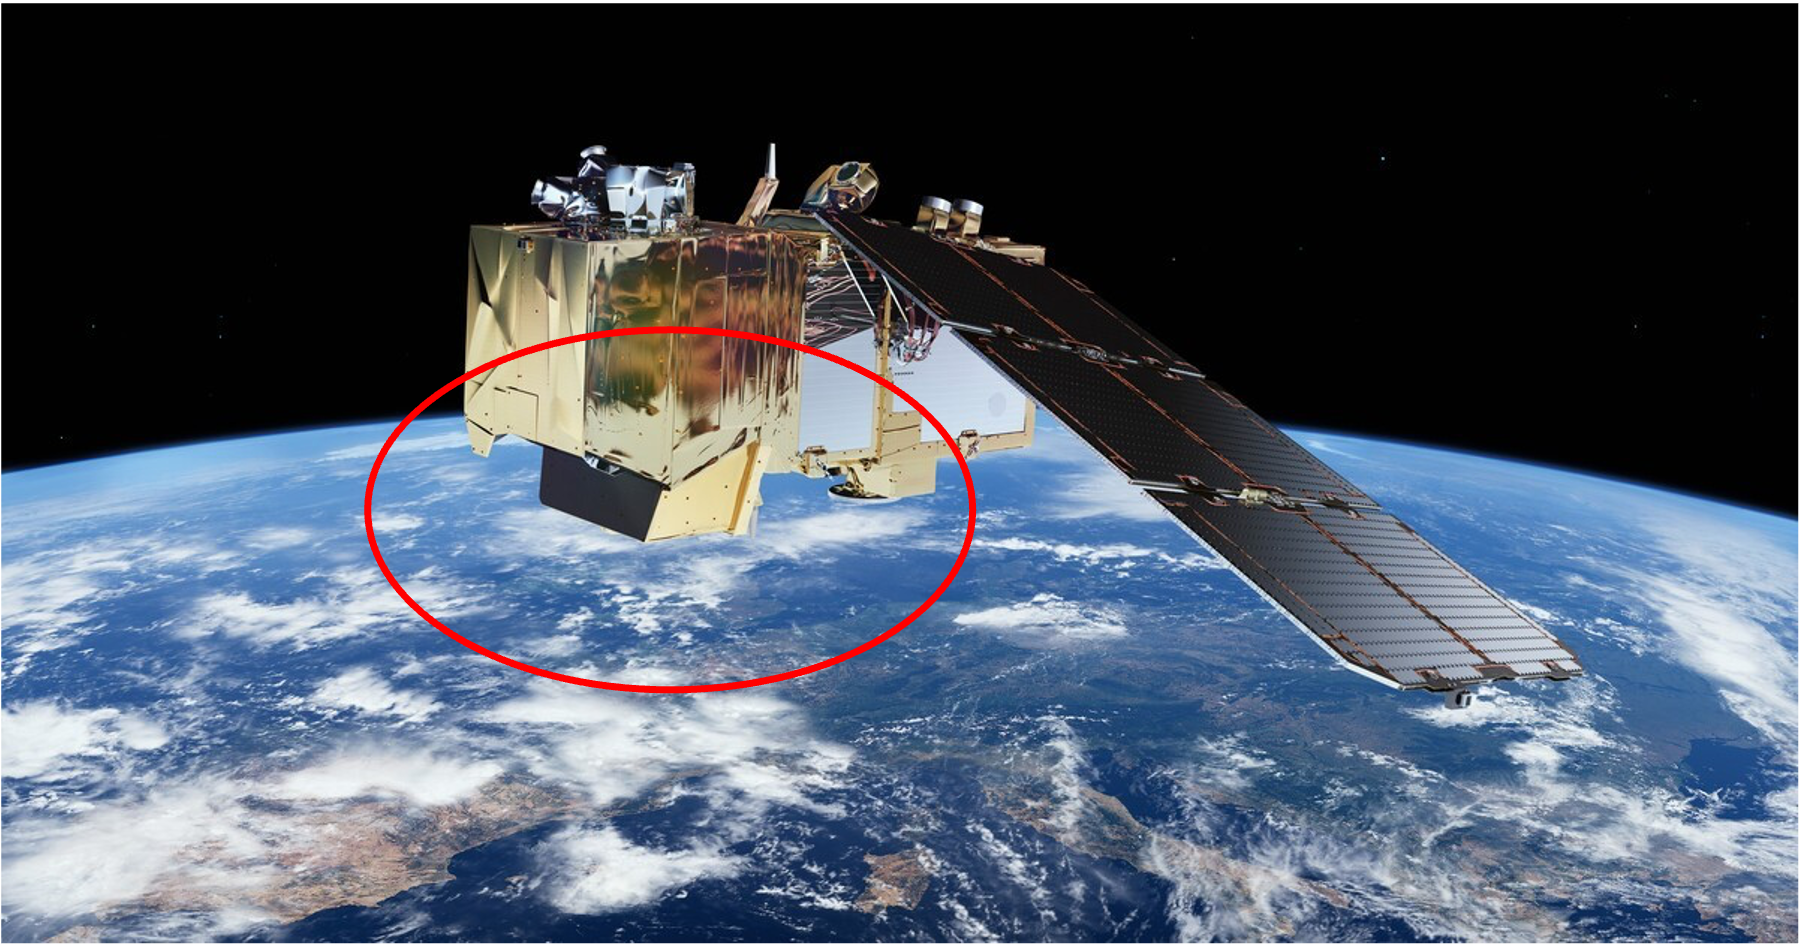
\includegraphics[width=0.9\linewidth]{figs/sentinel2.png}
  \caption{Sentinel-2 satellite in orbit. The red circle highlights the primary camera and sensor payload, which collects high-resolution observations of the Earth's surface and complementary signals (depending on the instrument and mission design) such as infrared, thermal, radar, and multispectral bands used to infer land cover, vegetation, and water.}
  \label{fig:sentinel2-payload}
\end{figure}

This thesis project aims to answer whether satellite imagery with geospatial foundation models is rich and dynamic enough to fill the gap in accurately collected population data. It evaluates two preeminent geospatial foundation models, the Clay foundation model of Earth data (2024) and Google's AlphaEarth model (2025), on the task of predicting population density in Mexico, which was chosen for its accessible census data and its relevance to a range of economic questions where population dynamics and census frequency are in tension. Mexico has experienced a recent surge in mining activity concentrated in states like Sonora and Zacatecas, generating labor migration that decennial census data cannot track at the frequency economic analysis requires. Workers move, towns swell, and the downstream mismatches in housing, services, and infrastructure provision accumulate before any enumeration can capture them. Similarly, the 2026 FIFA World Cup will be partially hosted in Mexico (in Mexico City, Guadalajara, and Monterrey), producing temporary but economically significant population concentrations whose impacts on local labor markets, retail, and municipal services traditional census data is structurally unable to isolate. These illustrate the broader problem of how economic shocks move people faster than the instruments we use to count them. Satellite-derived population estimates, updated at regular temporal cadences, could offer the kind of dynamic measurement these applications demand. This project therefore works towards distilling the limits and opportunities of using geospatial foundation models for exactly that purpose.

\subsection{Research Question}
\label{sub:researchque}
The guiding research questions of this thesis project are: 
\begin{enumerate}
  \item \textit{Can geospatial foundation models like AlphaEarth and Clay predict population density in Mexico at the AGEB and locality level? How does this performance change at a higher spatial scale?}
  \item \textit{Can these models predict population density changes over time?}
\end{enumerate}

\subsection{Key Findings}
This thesis yields three principal findings. 

First, geospatial foundation models predict cross-sectional population density with meaningful accuracy. Using AlphaEarth embeddings, an XGBoost prediction head explains $\approx73\%$ of variation in log population density at the polygon level ($R^2 = 0.727$), rising to $\approx88\%$ at the municipality level. Clay embeddings trail AlphaEarth at fine spatial scales but narrow the gap substantially after geographic aggregation. Both models exceed comparable benchmarks in the intercensal population estimation literature.

Second, prediction quality varies systematically across Mexico's geography. Large northern states consistently outperform smaller southern ones, driven primarily by differences in each state's typical polygon area.

Third, predicting the magnitude of decadal population change between 2010 and 2020 proves more challenging, with universally negative $R^2$ values on the change target. However, moderate Pearson correlations ($r \approx0.44$--$0.53$) indicate that the models reliably identify which areas are growing relative to which are shrinking, even when exact magnitudes remain out of reach.

\newpage

\section{Literature Review}

\paragraph{The evolution of machine learning architectures in remote sensing.} The methods used to extract socioeconomic information from remote sensing data have evolved rapidly. Early spatial analysis relied on shallow models with handcrafted features, such as simple linear regressions relating vegetation indices to crop yields or nighttime lights to economic growth. To better leverage spatial context, the field shifted toward Convolutional Neural Networks (CNNs), which methodologically learn complex spatial hierarchies, such as the density of buildings or urban infrastructure. Most recently, the field has seen a paradigm shift toward vision transformers (ViTs) and foundation models \parencite{zheng2025dynamic}. These architectures utilize cross-attention mechanisms to capture global context and are able to learn more complex spatial hierarchies. As such, they are proving to be state-of-the-art for many remote sensing tasks because they can dynamically weigh the relevance of different multimodal geospatial features depending on the region being analyzed \parencite{zheng2025dynamic}.

\paragraph{Task-specific population models.} Historically, population density prediction from satellite imagery has been done using task-specific models. These models are trained on a specific task and require manually curated features and architectures for each prediction target. An example of this is the use of CNNs trained specifically on satellite imagery to predict population density grids. This makes them difficult to adapt even across closely related tasks. At fine resolutions (30m), these models achieve an accuracy of $0.71$ in an urban Nanjing setting \parencite{SONG2019103580}. At a national or provincial level (250m), model performance improves significantly, achieving $R^2$ values up to $0.91$ \parencite{rs11222620}. But performance degrades when transferred to other cities and regions \parencite{tenzer_geospatial_2023}. \textcite{YAGOUB2024101122} found that when they tested their model trained on data from Al Ain, UAE on data from Abu Dhabi, UAE, the performance dropped from $R^2 = 0.89$ to $R^2 = 0.36$.

\paragraph{Geospatial foundation models.} To address this problem of model transferability across geographic contexts and temporal focuses, recent work is shifting from task-specific population models to general-purpose geospatial foundation models (GeoFMs). The introduction of frameworks like MOSAIKS demonstrated that raw imagery could be translated into compressed, task-agnostic features and reused across unlimited tasks using simple linear regression, making progress towards the transferability issue \parencite{sherman2026global}. Now is an exciting time to be working on GeoFMs, with many top labs releasing models that learn reusable embeddings of places from massive multimodal inputs. In 2024, the Clay foundation model of Earth data, which uses a ViT architecture to generate 768-dimensional latent space embeddings of the Earth's surface, was released as a project of the Radiant Earth non-profit \parencite{clayfoundation2026}. In 2025, Google released their AlphaEarth Foundations model \parencite{Brownetal2025}, which alongside Clay model make up the backbone of this project \parencite{proctor2025what}. While these models provide versatile embeddings, many like Clay are primarily pretrained on single-image views. Most recently, \textcite{zheng2026satellite} introduced the Tempov foundation model, which employs a bi-temporal self-supervised pretraining objective on three million Landsat image pairs. This approach forces the model to learn season-invariant semantics specifically optimized for tracking long-term changes in socioeconomic variables. Part of my research contribution is to assess the relative predictive performance of these different geospatial foundation models (namely, Clay and AlphaEarth), in addition to assessing the performance of GeoFMs against task-specific models for predicting population density. 

\paragraph{Expanding to socioeconomic outcomes.} The bulk of GeoFM work today is aimed at remote-sensing and environmental image tasks, with a growing secondary focus on health and socioeconomic outcomes where population is one component rather than the sole target. \textcite{cai_annual_2026} developed a 10\,m annual cropland dataset for Southeast Asia using AlphaEarth embeddings and found that the incorporation of AlphaEarth embeddings improved model performance by $5.81\%$. Beyond agriculture, researchers are also now using geospatial embeddings to predict highly complex human development metrics, such as predicting the UN's Human Development Index (HDI) at the micro-level \parencite{sherman2026global}, and asset wealth across data-scarce environments \parencite{zheng2025dynamic}. The integration of Earth observation machine learning with socioeconomic research has recently been formalized by \textcite{sakamoto2025scoping}, who categorize these efforts into five principal causal workflows: outcome imputation, image deconfounding, treatment effect heterogeneity, transportability, and causal discovery. A prominent example of the outcome imputation workflow is found in \textcite{ratledge2022using}, who utilized satellite-derived wealth measurements to evaluate the causal impact of electricity grid expansion in Uganda. Their study demonstrated that grid access improves village-level asset wealth by up to $0.15$ standard deviations, more than doubling growth rates relative to untreated areas.

\paragraph{The challenge of temporal prediction.} Despite these architectural advancements, predicting changes over time remains a notorious hurdle in the literature. While foundation models and CNNs can explain a vast majority of the spatial (cross-sectional) variation in socioeconomic outcomes between different locations, they often struggle to explain the temporal variation within those same locations over time \parencite{khachiyan2021using, zheng2025dynamic}. The core issue is that actual temporal changes over a few years are typically very small relative to cross-sectional differences, meaning that even slight observational noise in the satellite imagery or ground-truth label data can completely obscure the signal of change. \textcite{zheng2026satellite} further argue that existing models often fail because they lack temporal consistency in their representations, leading them to overfit to static geographic priors. \textcite{Burns2026} identifies that in GeoFM embedding spaces, large interannual differences can arise from climate variability or structural context rather than actual surface transitions. She found that magnitude-only comparisons of embeddings (e.g., calculating the delta between two years of embeddings) can fail to distinguish between distinct types of change that produce similar vector magnitudes, leading to fragmented predictions in heterogeneous landscapes. By explicitly contrasting multi-seasonal image pairs during pretraining, models like Tempov have begun to address this by successfully disentangling genuine socioeconomic evolution from seasonal phenological noise, maintaining robust predictive power for decadal changes where other baselines deteriorate.

\paragraph{Predicting historical population shifts over time.} Within this temporal prediction landscape, predicting highly localized historical population shifts remains a sparse and unique niche. Traditionally, historical population estimation has relied on top-down approaches that disaggregate outdated census data. Bottom-up models that directly predict local population changes over time are rare. \textcite{khachiyan2021using} provides the most notable benchmark in this space. They successfully trained a CNN on daytime Landsat imagery to predict decadal changes in population at the 1.2 km and 2.4 km resolutions. They achieved an $R^2$ of $0.46$ for historical population growth rate prediction, which while good is not at the statistical rigor of other cross-sectional predictions. Moreover, because their model was trained from scratch on specific variables, it lacks task-agnostic flexibility that a GeoFM can provide. Little has been explored at the intersection of foundation models and population density prediction, let alone temporal change in population prediction. Most GeoFM work related to population density focuses on cross-sectional estimations, like \textcite{metz2025application} who found an $R^2$ of $0.63$--$0.64$ for population density in Malawi. Even then, the quantity of work with GeoFMs for population density prediction pales in comparison to the amount of work with task-specific models.

\paragraph{This project's intervention.}
My project aims to bridge the aforementioned gap in the literature by leveraging state-of-the-art GeoFMs like AlphaEarth and Clay to predict not just static population density in census years but also the viability of these models to predict dynamic population changes. By shifting from task-specific CNNs to GeoFMs, this approach aims to maintain the high temporal accuracy seen in \textcite{khachiyan2021using} while drastically improving model transferability. When investigating the ability of these models to predict population density changes over time, I adopt a baseline-anchored approach (e.g., using 2010 embeddings to predict 2020 labels rather than using the difference between the labels to predict the difference in population density between 2010 and 2020). This attempts to preserve the historical environmental context and avoid the pitfalls of magnitude-only representations of embedding changes that \textcite{Burns2026} identified. To handle the heavily skewed distribution of population data, this project employs a log-then-inverse-transform pipeline. This methodology is well-supported by the literature. \textcite{khachiyan2021using} explicitly modeled the ``log of total population'', and \textcite{proctor2025what} utilized automated tuning pipelines that selected log transformations for prediction targets to optimize foundation model performance. This thesis follows this methodological precedent and also trains on log-transformed labels. Finally, this project tries to stay close to the insight of \textcite{ratledge2022using}, who emphasize that upstream model optimization must be carefully aligned with downstream tasks, as maximizing standard predictive metrics like $R^2$ can sometimes lead to increased bias in final inferences. 

\newpage

\section{Methodology}
\label{sec:methodology}

\subsection{Dataset}
Even though this project's geographic focus is on Mexico primarily because of the ease of access to high-quality census data and satellite imagery, a substantial amount of data gathering and preparation still went into gathering ground-truth label data.

\subsubsection{Census Data Source}

The census ground truth labels came from the INEGI (Instituto Nacional de Estadística y Geografía) website.\footnote{INEGI website: https://www.inegi.org.mx/programas/ccpv/2020/.} The data was downloaded as a CSV file for each state, and then combined into a single combined CSV file. The data was then cleaned and prepared for analysis.

I focused on the urban AGEB and rural locality level data because it was the most granular geospatial unit that census data was available for (see Table \ref{tab:inegi_hierarchy} for more on the INEGI geospatial units). I also focused on the 2020 and 2010 census data because it was the most recent data that was available, and this recency meant that I had access to better quality satellite imagery, which would hypothetically help with better predictions and embedding quality. 

An important thing to note is that urban AGEBs and rural localities are mutually exclusive and together cover the populated areas of interest. Urban AGEBs are a more granular level of geography of an urban locality; in other words, there are $\ge 1$ urban AGEB polygons within a single urban locality polygon.

\begin{table}[H]
  \centering
  \caption{INEGI National Geostatistical Framework (Marco Geoestadístico). \protect\colorbox{teal!15}{Highlighted} text indicates the geographic units this project focuses on.}
  \label{tab:inegi_hierarchy}
  \renewcommand{\arraystretch}{1.15}
  \setlength{\tabcolsep}{8pt}
  \begin{tabularx}{\linewidth}{@{}
    >{\raggedright\arraybackslash}p{0.14\linewidth}
    >{\raggedright\arraybackslash}p{0.26\linewidth}
    >{\centering\arraybackslash}p{0.10\linewidth}
    >{\raggedright\arraybackslash}p{0.50\linewidth}
  @{}}
    \toprule
    \textbf{Level} & \textbf{Official Name} & \textbf{Census data?} & \textbf{Description} \\
    \midrule
    State & Entidad Federativa & $\checkmark$ & The 32 sovereign states of Mexico. \\
    Municipality & Municipio / Demarcación & $\checkmark$ & Political-administrative subdivisions. \\
    Locality & Localidad Geoestadística & $\checkmark$ & \textit{Urban:} $\ge$ 2{,}500 people or seat of power. \newline \colorbox{teal!15}{\strut\textit{Rural:} $<$ 2{,}500 people (point-based).} \\
    AGEB & Área Geoestadística Básica & $\checkmark$ & \colorbox{teal!15}{\strut\textit{Urban:} Nested in localities; 1--50 blocks.} \newline \textit{Rural:} Large polygon (avg.\ 10k ha). \\
    Manzana & Manzana Geoestadística & $\times$ & Smallest unit. Defined by streets/features. Mostly used in urban contexts. \\
    \bottomrule
  \end{tabularx}
\end{table}

For context on the size of these census datasets, the locality-level dataset for 2020 ended up having 189,433 entries and the AGEB-level dataset had 64,313 entries. However, not all these entries could be used for the final training/testing set, which was limited by what shapefile polygons I had access to (discussed in Section \ref{subsub:shpsource}).

\subsubsection{Shapefile Source}
\label{subsub:shpsource}

The shapefiles corresponding to each year's census data was also downloaded from the INEGI website. Each folder contained shapefiles for all the various geospatial units, but I only focused on the urban AGEB and rural locality level data. Notably, for the 2010 census, there were no shapefile polygon data for the rural localities. This limited the size of that dataset (see Table \ref{tab:shapefile_polygon_counts} for full breakdown of each polygon dataset and Figure \ref{fig:polygon_coverage_2010_2020} for a visual of the spatial coverage of the polygon datasets).

\begin{table}[H]
  \centering
  \caption{Shapefile polygon counts by year (focus breakdown).
  \newline \footnotesize \textit{Notes:} For 2020, AGEB total = 81{,}451 (urban = 63{,}982; rural = 17{,}469) and Localidad total = 50{,}308 (rural = 45{,}397; urban = 5{,}011). For 2010, only urban AGEB polygons were available (56{,}195).}
  \label{tab:shapefile_polygon_counts}
  \renewcommand{\arraystretch}{1.15}
  \setlength{\tabcolsep}{7pt}
  \begin{tabularx}{\linewidth}{@{}
    >{\raggedright\arraybackslash}p{0.12\linewidth}
    >{\centering\arraybackslash}p{0.22\linewidth}
    >{\centering\arraybackslash}p{0.22\linewidth}
    >{\centering\arraybackslash}p{0.22\linewidth}
  @{}}
    \toprule
    \textbf{Year} &
    \textbf{Total polygons} &
    \textbf{Urban AGEB} &
    \textbf{Rural Localidad} \\
    \midrule
    2020 & 109{,}379 & 63{,}982 & 45{,}397 \\
    2010 & 56{,}195 & 56{,}195 & --- \\
    \bottomrule
  \end{tabularx}
\end{table}

\begin{figure}[H]
  \centering
  \begin{minipage}[t]{0.49\linewidth}
    \centering
    {\setlength{\fboxsep}{0pt}\fbox{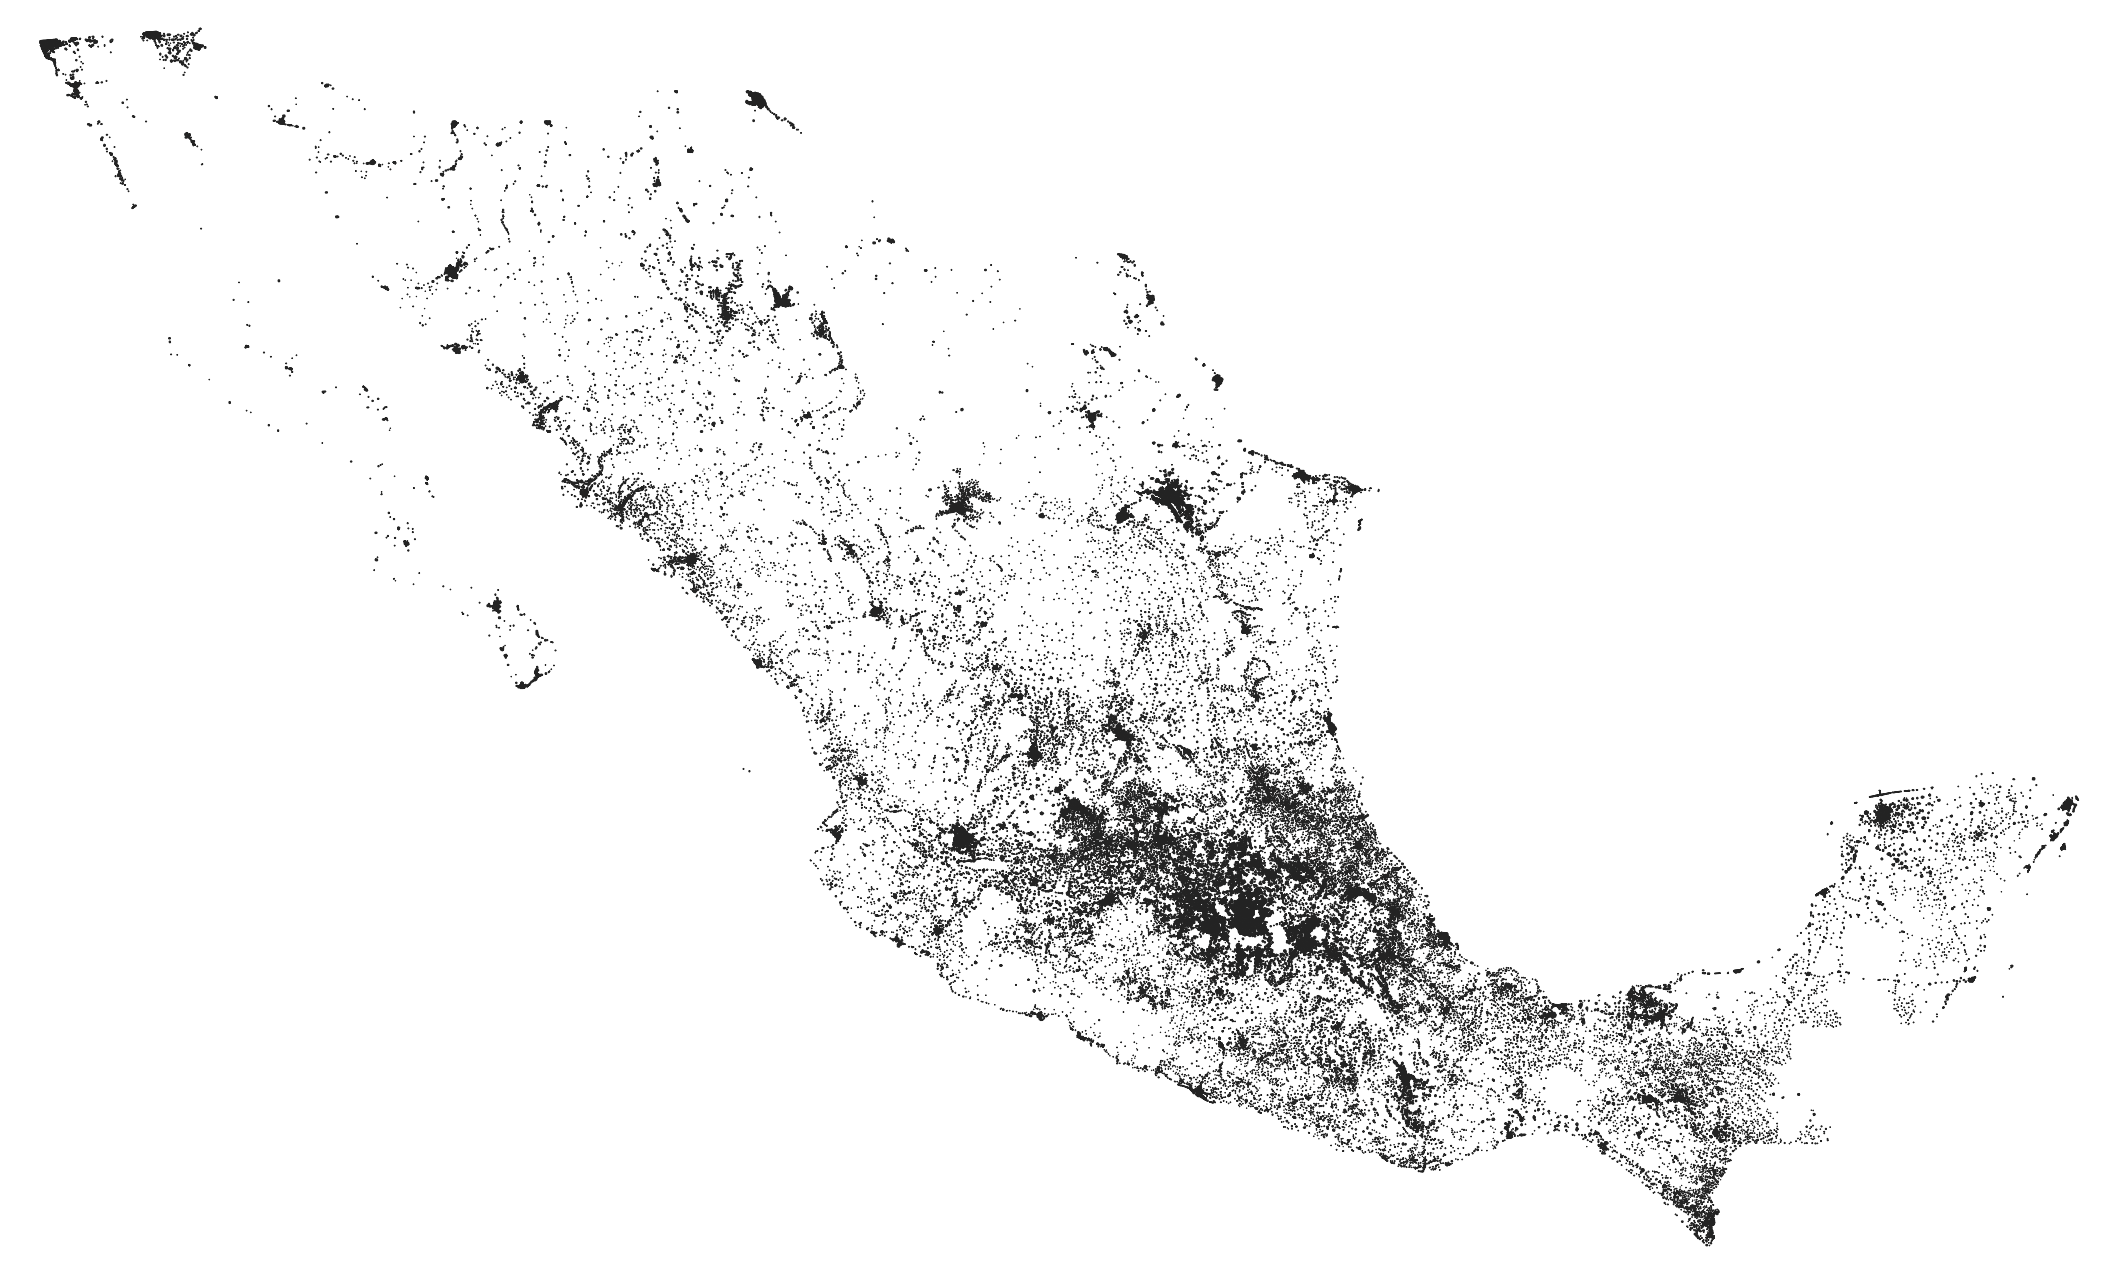
\includegraphics[width=\linewidth]{figs/2020_merged_agebu_rurall.png}}}
  \end{minipage}\hfill
  \begin{minipage}[t]{0.49\linewidth}
    \centering
    {\setlength{\fboxsep}{0pt}\fbox{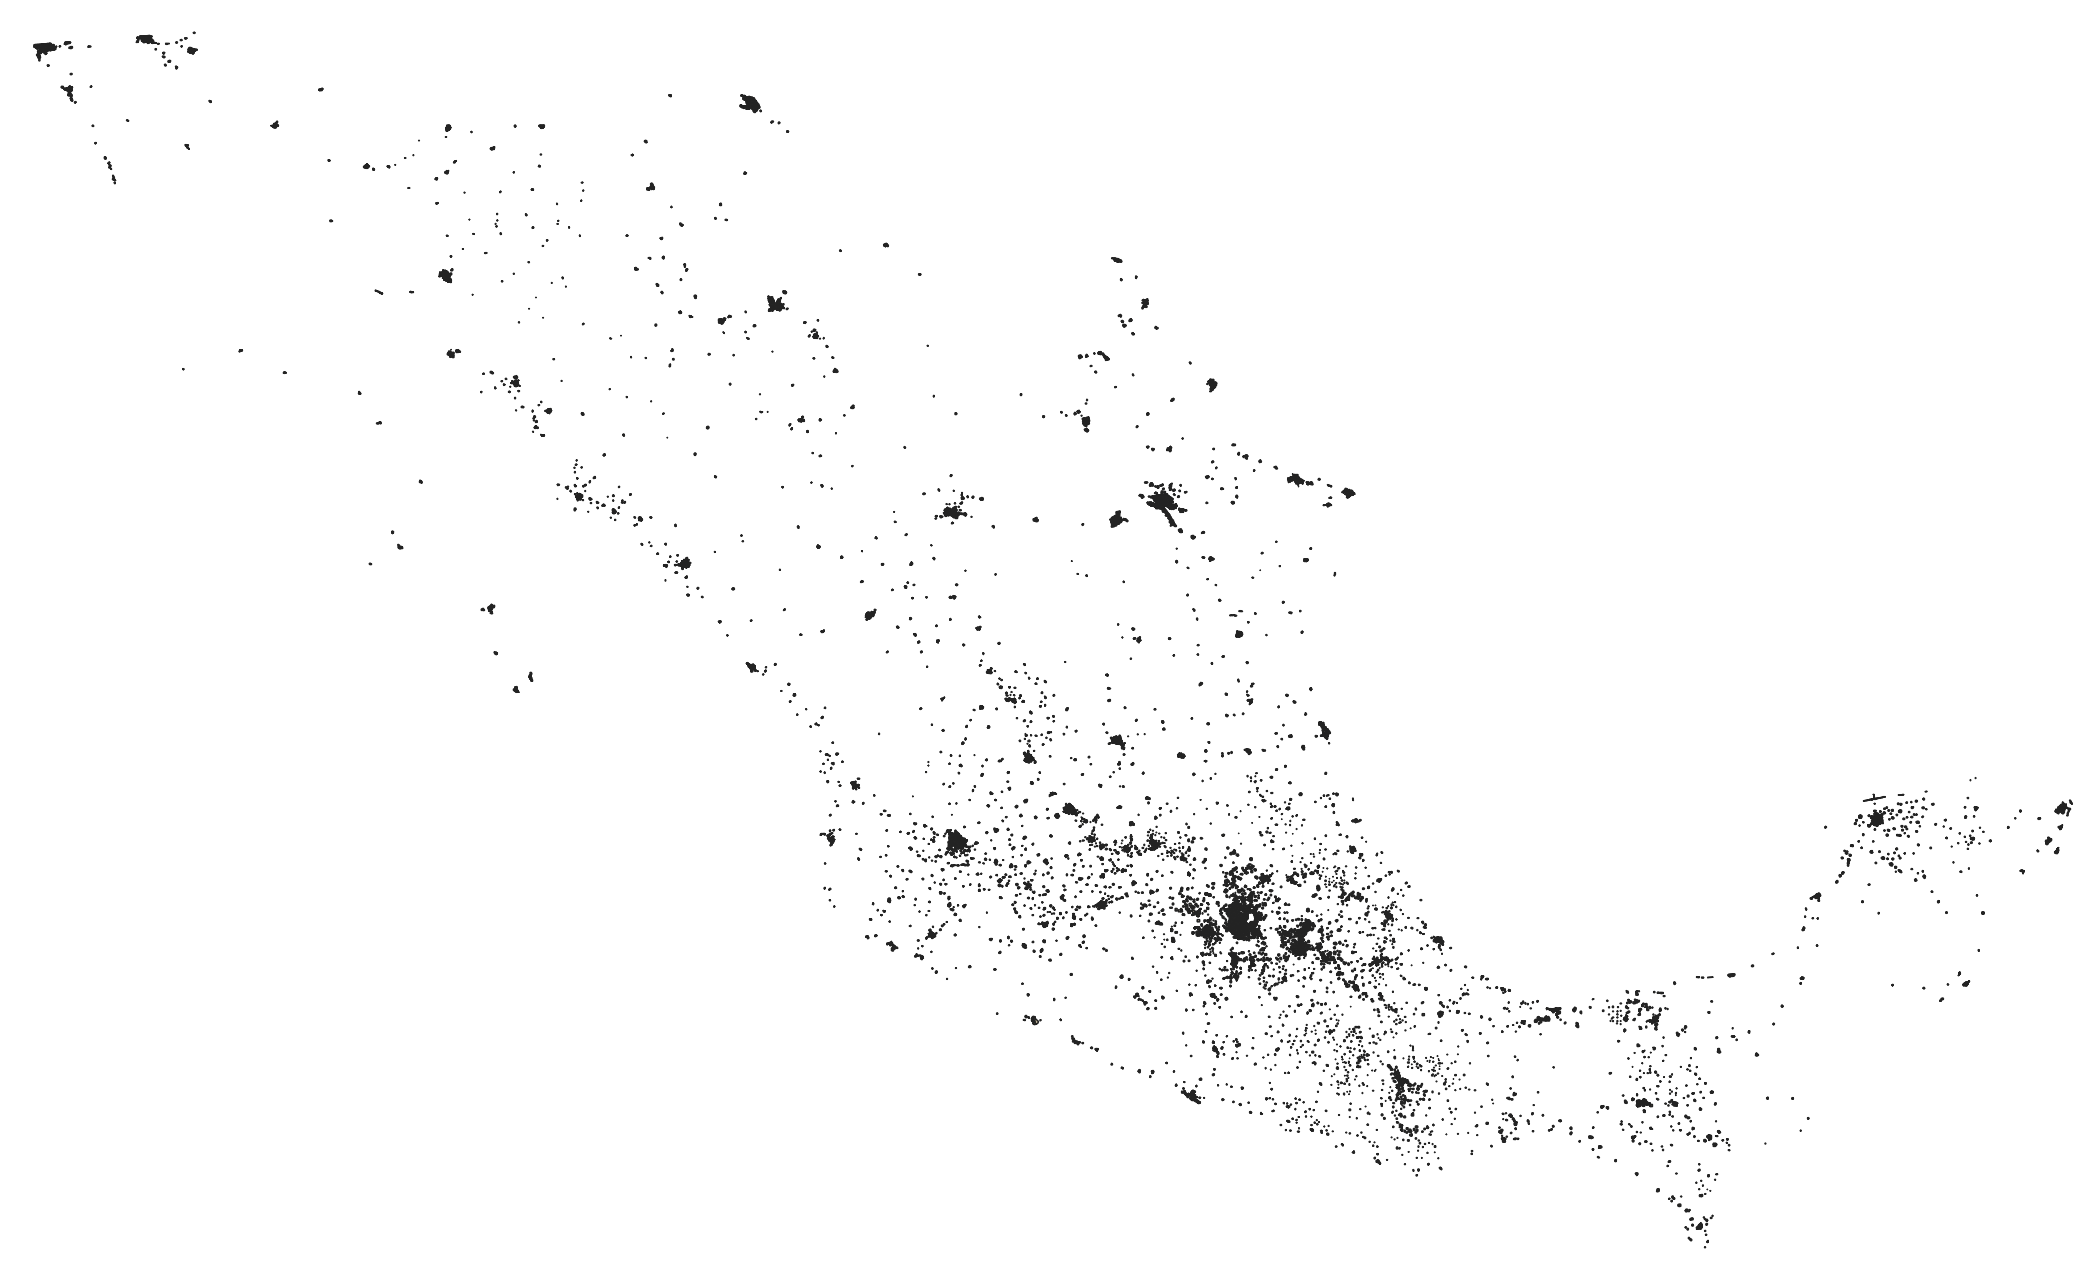
\includegraphics[width=\linewidth]{figs/2010_ageb_u.png}}}
  \end{minipage}
  \caption{Spatial coverage of the polygon datasets used in this project. \textbf{Left:} 2020 merged shapefile (urban AGEBs and rural localities). \textbf{Right:} 2010 urban AGEBs only. The denser and more geographically complete 2020 map reflects the inclusion of rural locality polygons, which are not available in the 2010 shapefiles (see Table~\ref{tab:shapefile_polygon_counts}).}
  \label{fig:polygon_coverage_2010_2020}
\end{figure}

\subsubsection{Merging the Census Data with the Shapefiles}

The next step was to clean the census data and merge it with the shapefiles. To help merge the data, I created the CVEGEO item (see Table~\ref{tab:cvegeo_structure}), which is a unique identifier for each polygon. To clean the census data, I only retained population-relevant columns and also computed log-transformed population measures to help handle the heavily skewed distribution of population data (see Figure \ref{fig:eda_raw_popden_population_linear_logx} in Section \ref{subsub:eda} below). To account for the degenerate case that population is 0, I calculated $\ln{(popden + 1)}$ every time I refer to log-transformed population measures.

\begin{table}[H]
  \centering
  \caption{How the INEGI Geostatistical Key (CVEGEO) is constructed}
  \label{tab:cvegeo_structure}
  \renewcommand{\arraystretch}{1.15}
  \setlength{\tabcolsep}{8pt}
  \begin{tabularx}{\linewidth}{@{} l l c @{}}
    \toprule
    \textbf{Geographic Unit} & \textbf{CVEGEO concatenation} & \textbf{Digits} \\
    \midrule
    Locality (Urban/Rural) & ENT + MUN + LOC & 9 \\
    Urban AGEB & ENT + MUN + LOC + AGEB & 13 \\
    Rural AGEB & ENT + MUN + AGEB & 9 \\
    \bottomrule
  \end{tabularx}
\end{table}

I used QGIS to load in the shapefiles alongside the cleaned census data CSVs and then joined the layers together. This produced a single shapefile with the population data attached to each polygon.

After merging, I calculated the area of each polygon in square kilometers and also calculated the population density by dividing the total population of a polygon by the area of the polygon. This value was also then log-transformed to help with the skewed distribution of population data. I use the population density rather than absolute population because the polygon areas for urban AGEB and rural localities varied drastically (min. area: 0.0003 square km; max. area: 36.4128 square km).

\subsubsection{Exploratory Data Analysis}
\label{subsub:eda}
The need to log the population and population-density targets became exceptionally clear when plotting both labels on their original scales vs. log scales. Under a linear horizontal axis, the histograms positive skewness and concentrate almost all mass at the left. A $\log_{10}$-scaled axis, however, linearizes the relationship and reveals the underlying distribution of the right tail, ensuring that high-density urban outliers do not disproportionately dominate the model (Figure~\ref{fig:eda_raw_popden_population_linear_logx}).

The following analysis was performed on the 2020 census dataset, but similar analysis can be performed on the 2010 census dataset and similar results were observed.

\begin{figure}[H]
  \centering
  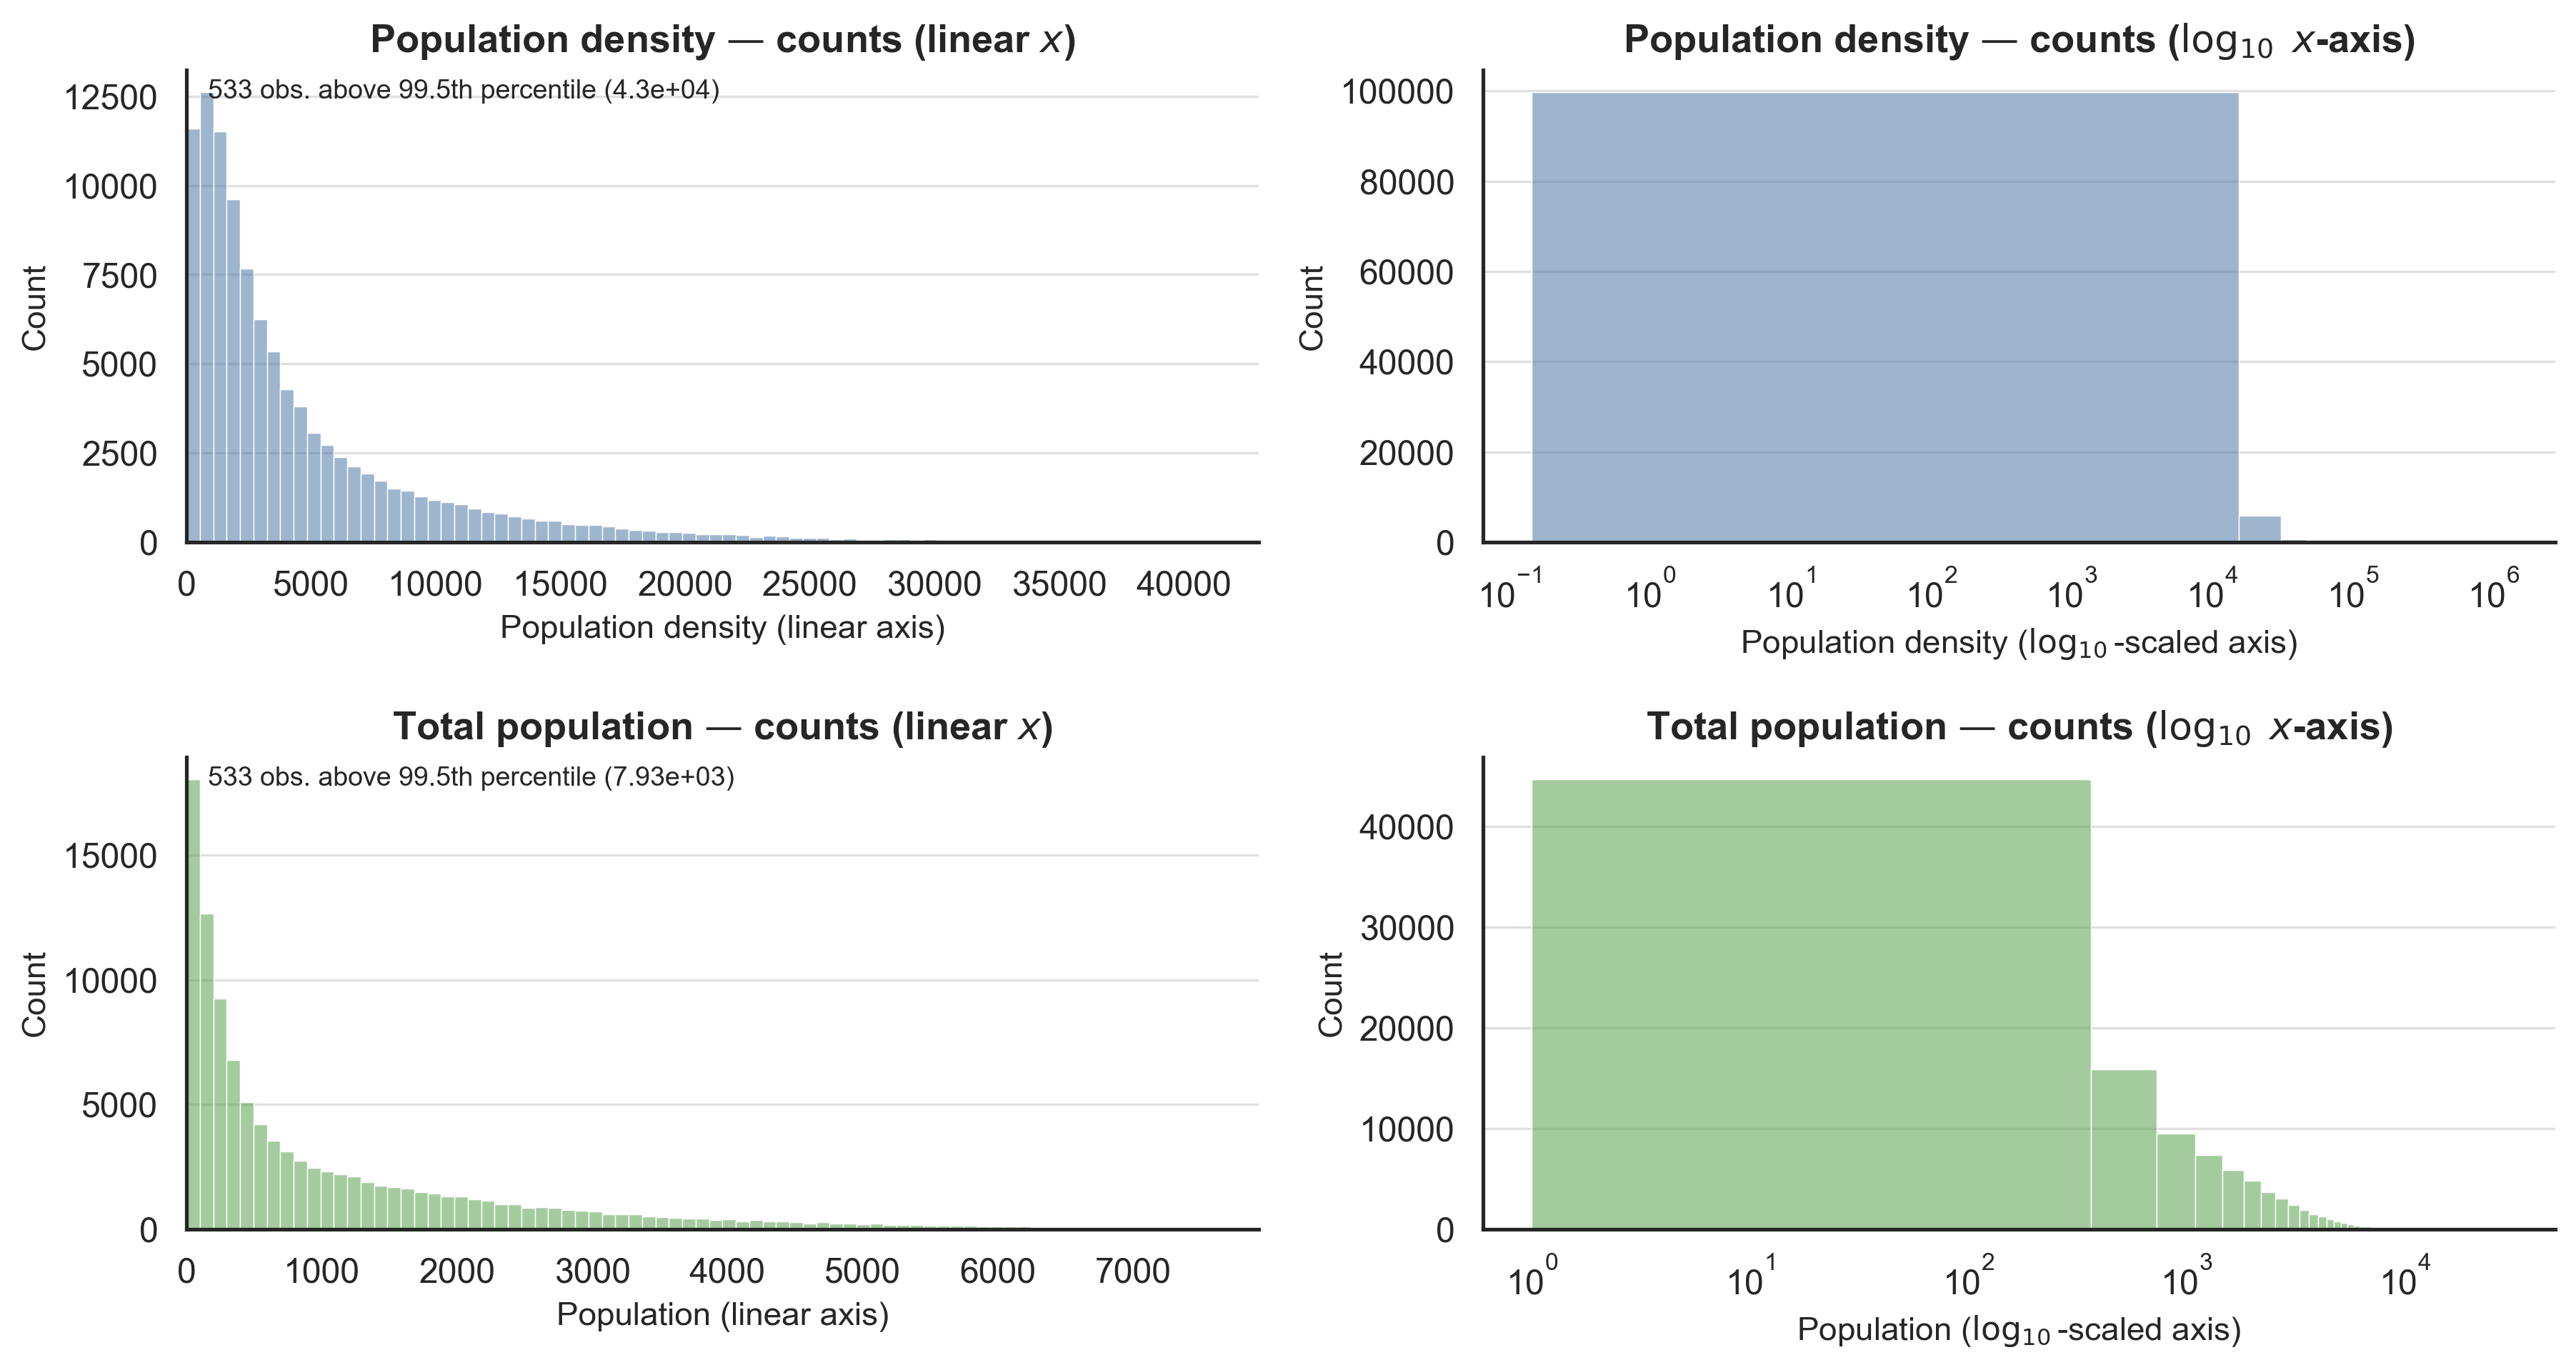
\includegraphics[width=\linewidth]{figs/eda_raw_popden_and_population_logx.png}
  \caption{Original-scale population density and total population (filtered sample), as histograms of bin counts. \textbf{Left column:} linear $x$-axis with bins restricted to the 99.5th percentile so the bulk of each distribution is readable; the panel text reports how many observations exceed that cutoff. \textbf{Right column:} the same quantities on a $\log_{10}$ horizontal axis so the full range is visible.}
  \label{fig:eda_raw_popden_population_linear_logx}
\end{figure}

Analyzing the merged shapefile with census data, I noticed that the data was skewed towards having many entries with log population density equal to $0$, which (due to our definition of log population density) meant that there were many entries in the dataset (i.e., urban AGEB or rural locality polygons) with population equal to 0 (see Figure \ref{fig:popden_filtering_eda}). I decided to ignore these because their inclusion would result in a zero-inflated distribution that significantly biases the regression. Since the research objective is to model the variance in human settlement density, including a large mass of zero-valued observations---which often represent non-residential land uses like industrial zones, airports, or conservation areas—would force the model to prioritize a binary ``presence vs. absence'' classification task rather than the nuanced estimation of population density.

This filtering ultimately led to roughly 3\% of the entries being removed, including not just the zero-valued population density entries but also any NaN entries (Figure \ref{tab:popden_filtering_summary}).

\begin{table}[H]
  \centering
  \caption{Summary statistics for ln(population density) before and after filtering zero-valued targets}
  \renewcommand{\arraystretch}{1.15}
  \setlength{\tabcolsep}{8pt}
  \begin{tabular}{@{}l r r r r r@{}}
    \toprule
    \textbf{Dataset} & \textbf{Rows} & \textbf{Share of total} & \textbf{Min} & \textbf{Median} & \textbf{99th pct.} \\
    \midrule
    Raw & 109{,}379 & 1.000 & 0.000 & 3.422 & 4.48900 \\
    Filtered & 106{,}564 & 0.974 & 0.059 & 3.433 & 4.49337 \\
    \bottomrule
  \end{tabular}
  \label{tab:popden_filtering_summary}
\end{table}

\begin{figure}[H]
  \centering
  \begin{minipage}[t]{0.495\linewidth}
    \centering
    {\setlength{\fboxsep}{0pt}\fbox{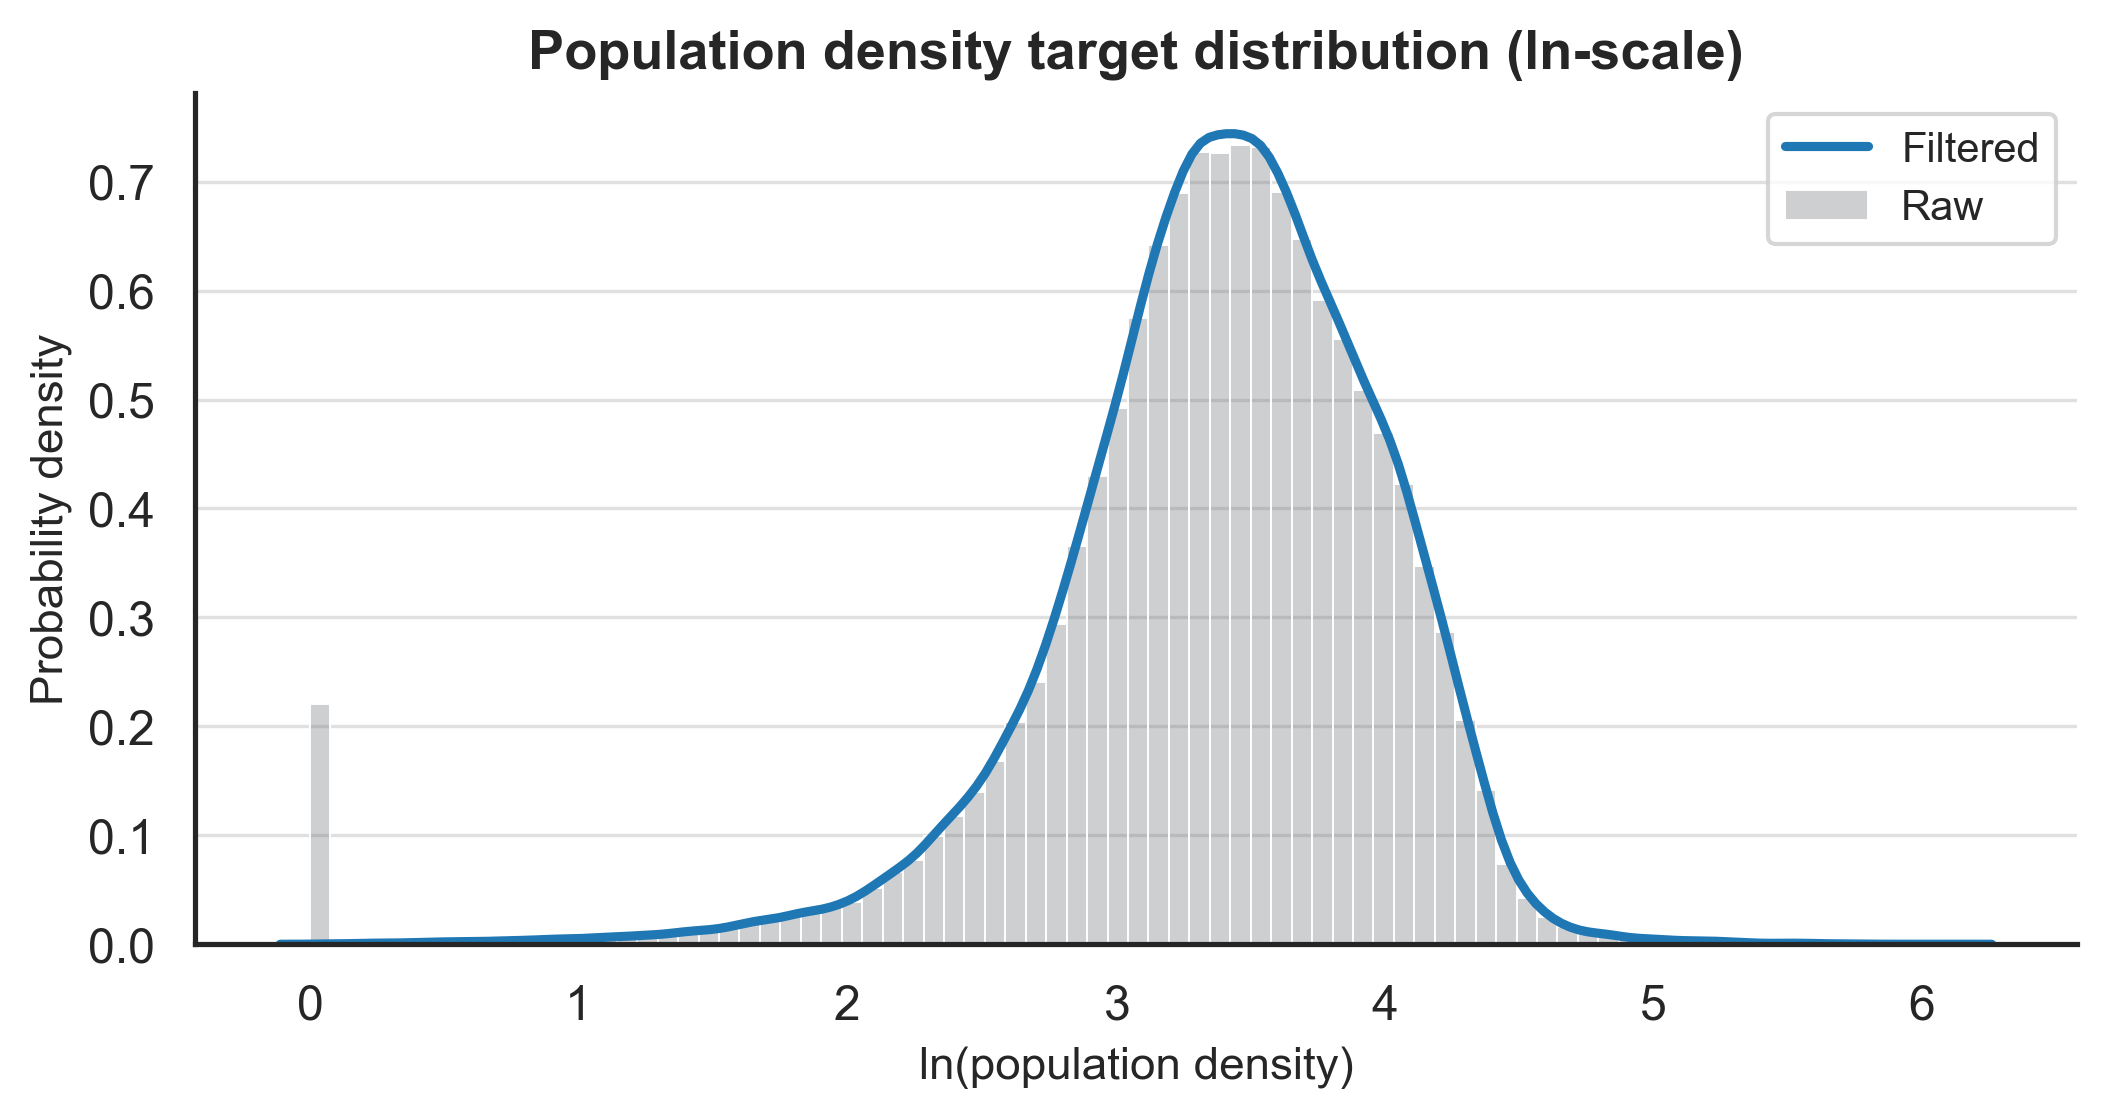
\includegraphics[width=1.02\linewidth]{figs/eda_log_popden_distribution.png}}}
    \vspace{0.25em}
    \caption*{\footnotesize (a) Probability density (shape).}
  \end{minipage}\hfill
  \begin{minipage}[t]{0.495\linewidth}
    \centering
    {\setlength{\fboxsep}{0pt}\fbox{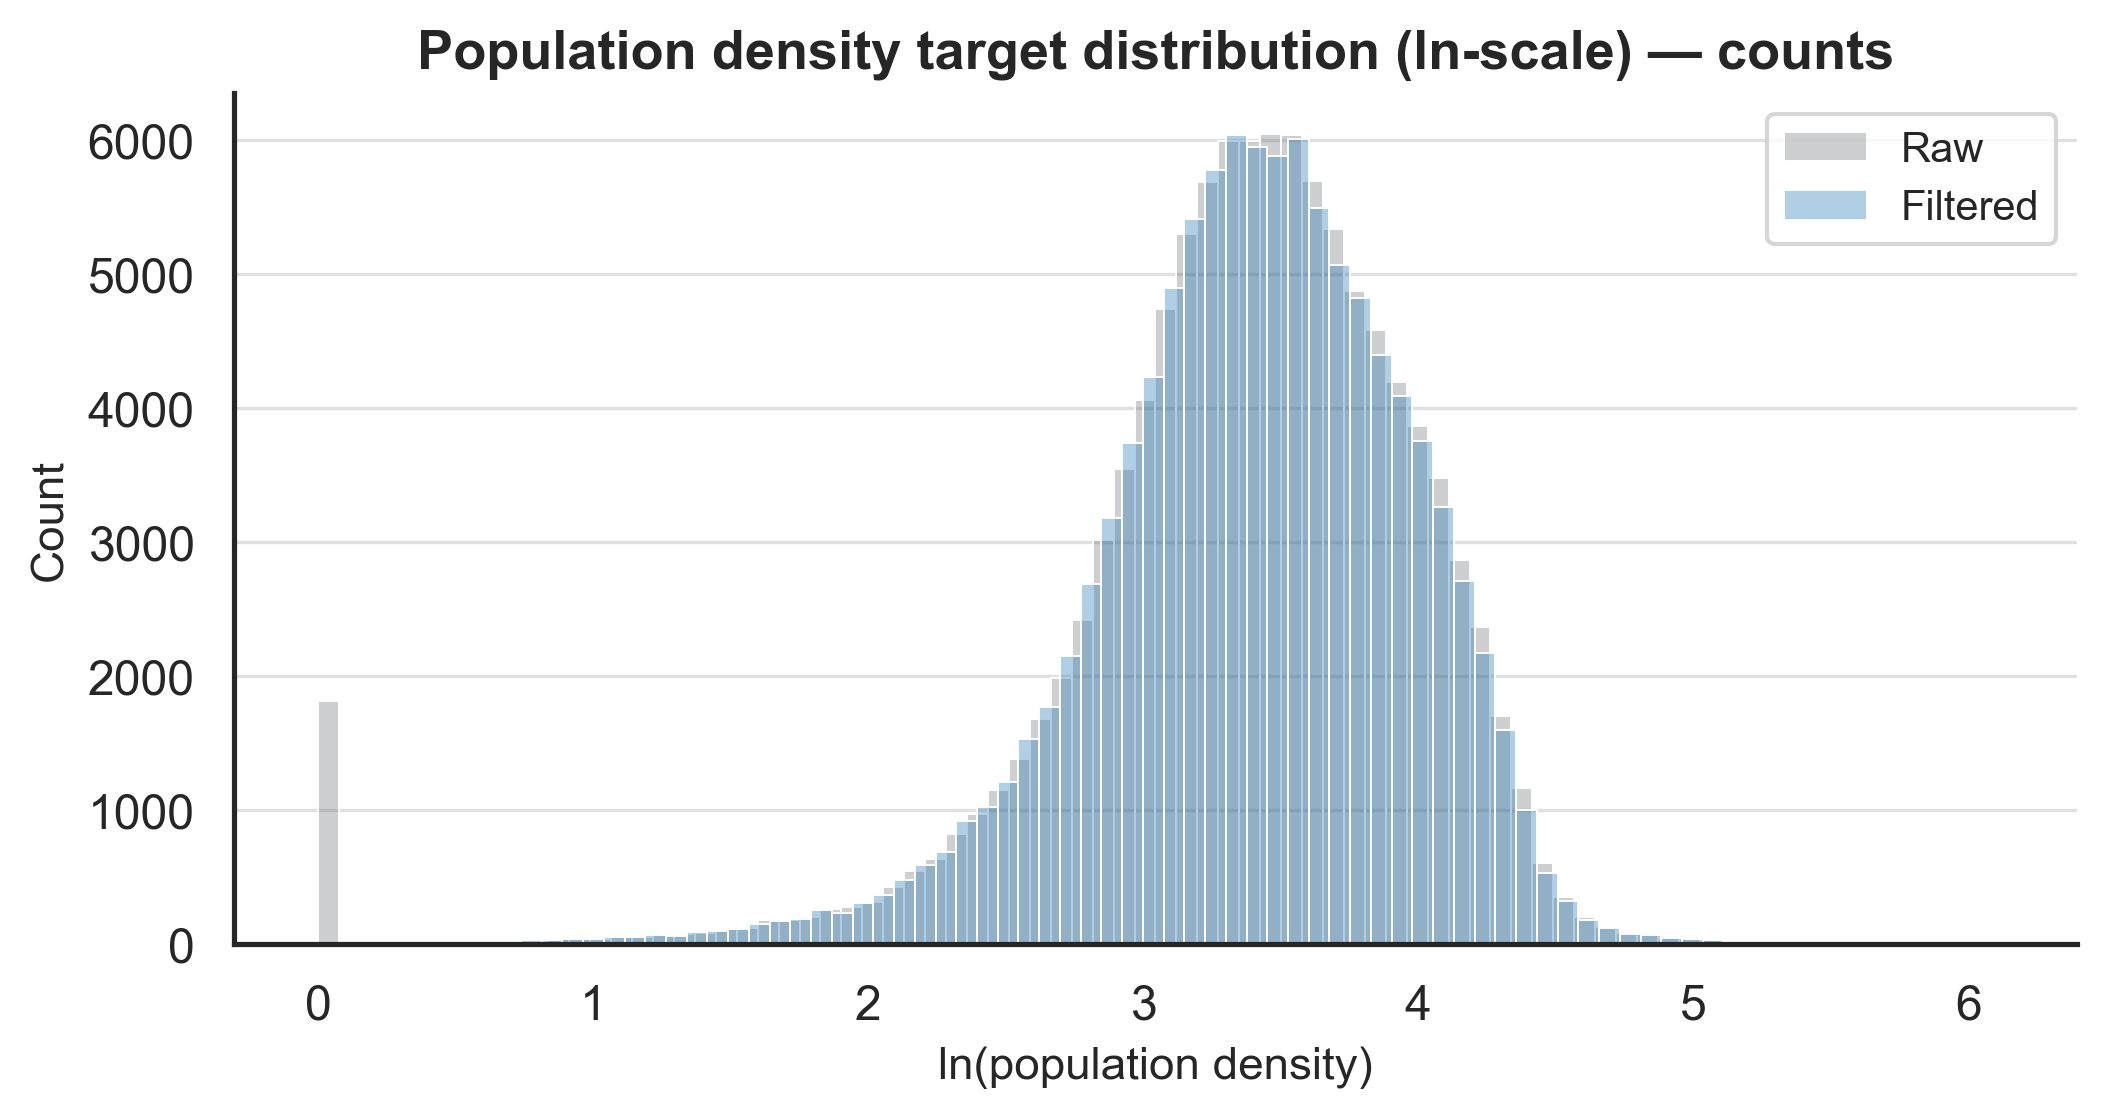
\includegraphics[width=1.02\linewidth]{figs/eda_log_popden_counts.png}}}
    \vspace{0.25em}
    \caption*{\footnotesize (b) Raw counts (mass at 0).}
  \end{minipage}
  \caption{Distribution of ln(population density) in the merged dataset, before and after filtering out placeholder zero-valued targets. Panel (a) emphasizes distributional shape via probability density; panel (b) shows raw counts, highlighting the removed mass at exactly 0.}
  \label{fig:popden_filtering_eda}
\end{figure}

Another interesting observation was that while the number of polygons available for each state varied significantly (with larger states intuitively having more polygons; see Figure \ref{fig:eda_state_counts_filtered}), the distribution of log population density was more or less similar across all states (see Figure \ref{fig:eda_state_log_popden_quantiles}). This provided evidence for the robustness of this dataset to be used to train the AlphaEarth and Clay models to different geographic contexts. The one outlier was Ciudad de México, which had a much higher median log population density (4.265) than any other state. This is because Ciudad de México is a very dense urban area with many small polygons, which results in a higher median log population density. 

\begin{figure}[H]
  \centering
  {\setlength{\fboxsep}{0pt}{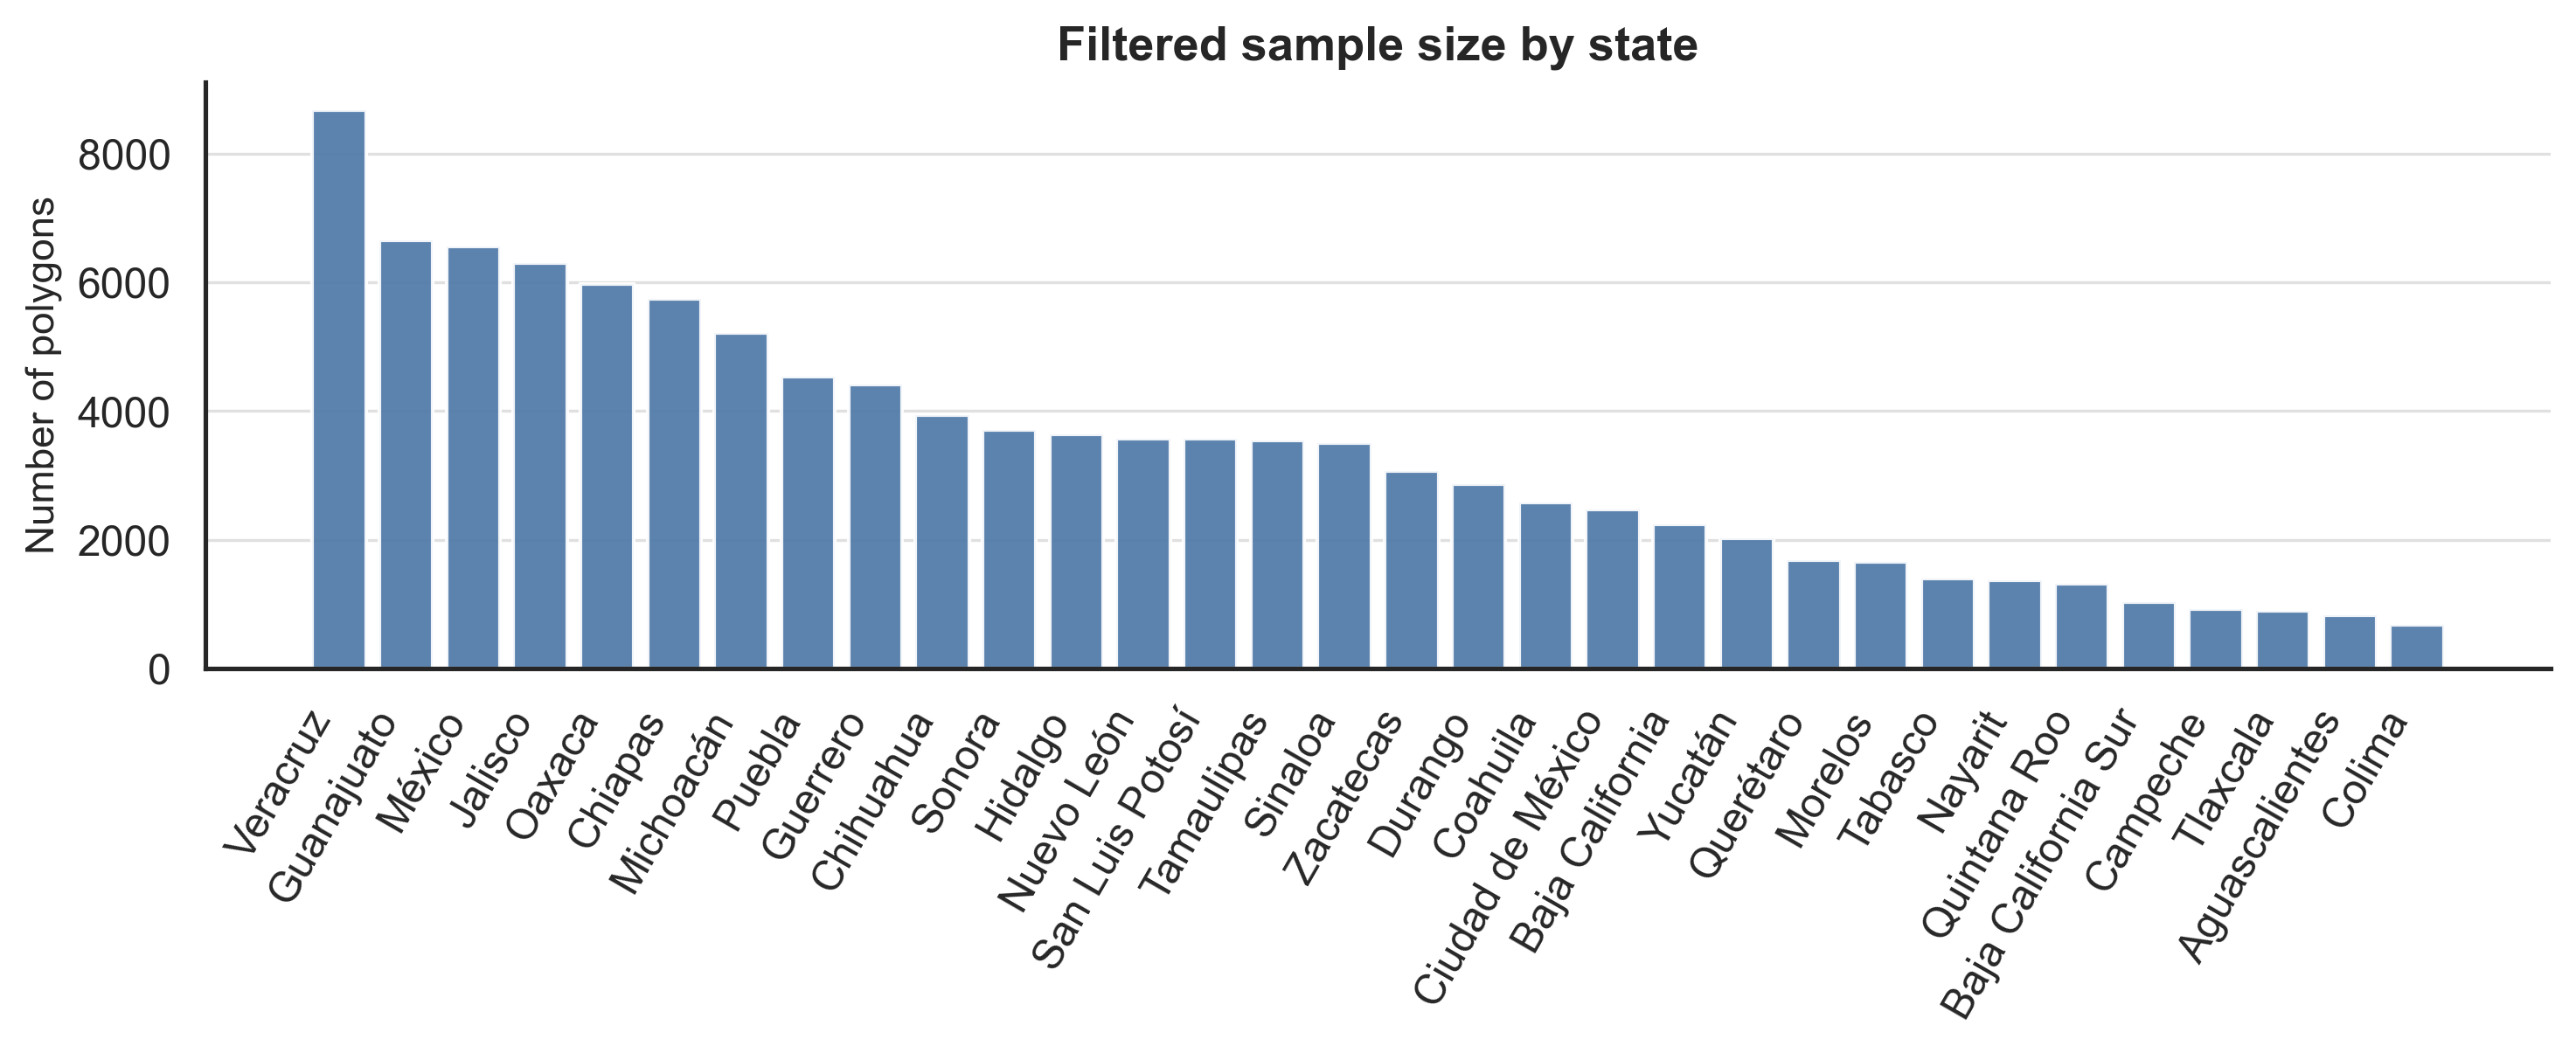
\includegraphics[width=0.8\linewidth]{figs/eda_state_counts_filtered.png}}}
  \caption{Filtered sample size by state (number of polygons).}
  \label{fig:eda_state_counts_filtered}
\end{figure}

\begin{figure}[H]
  \centering
  {\setlength{\fboxsep}{0pt}{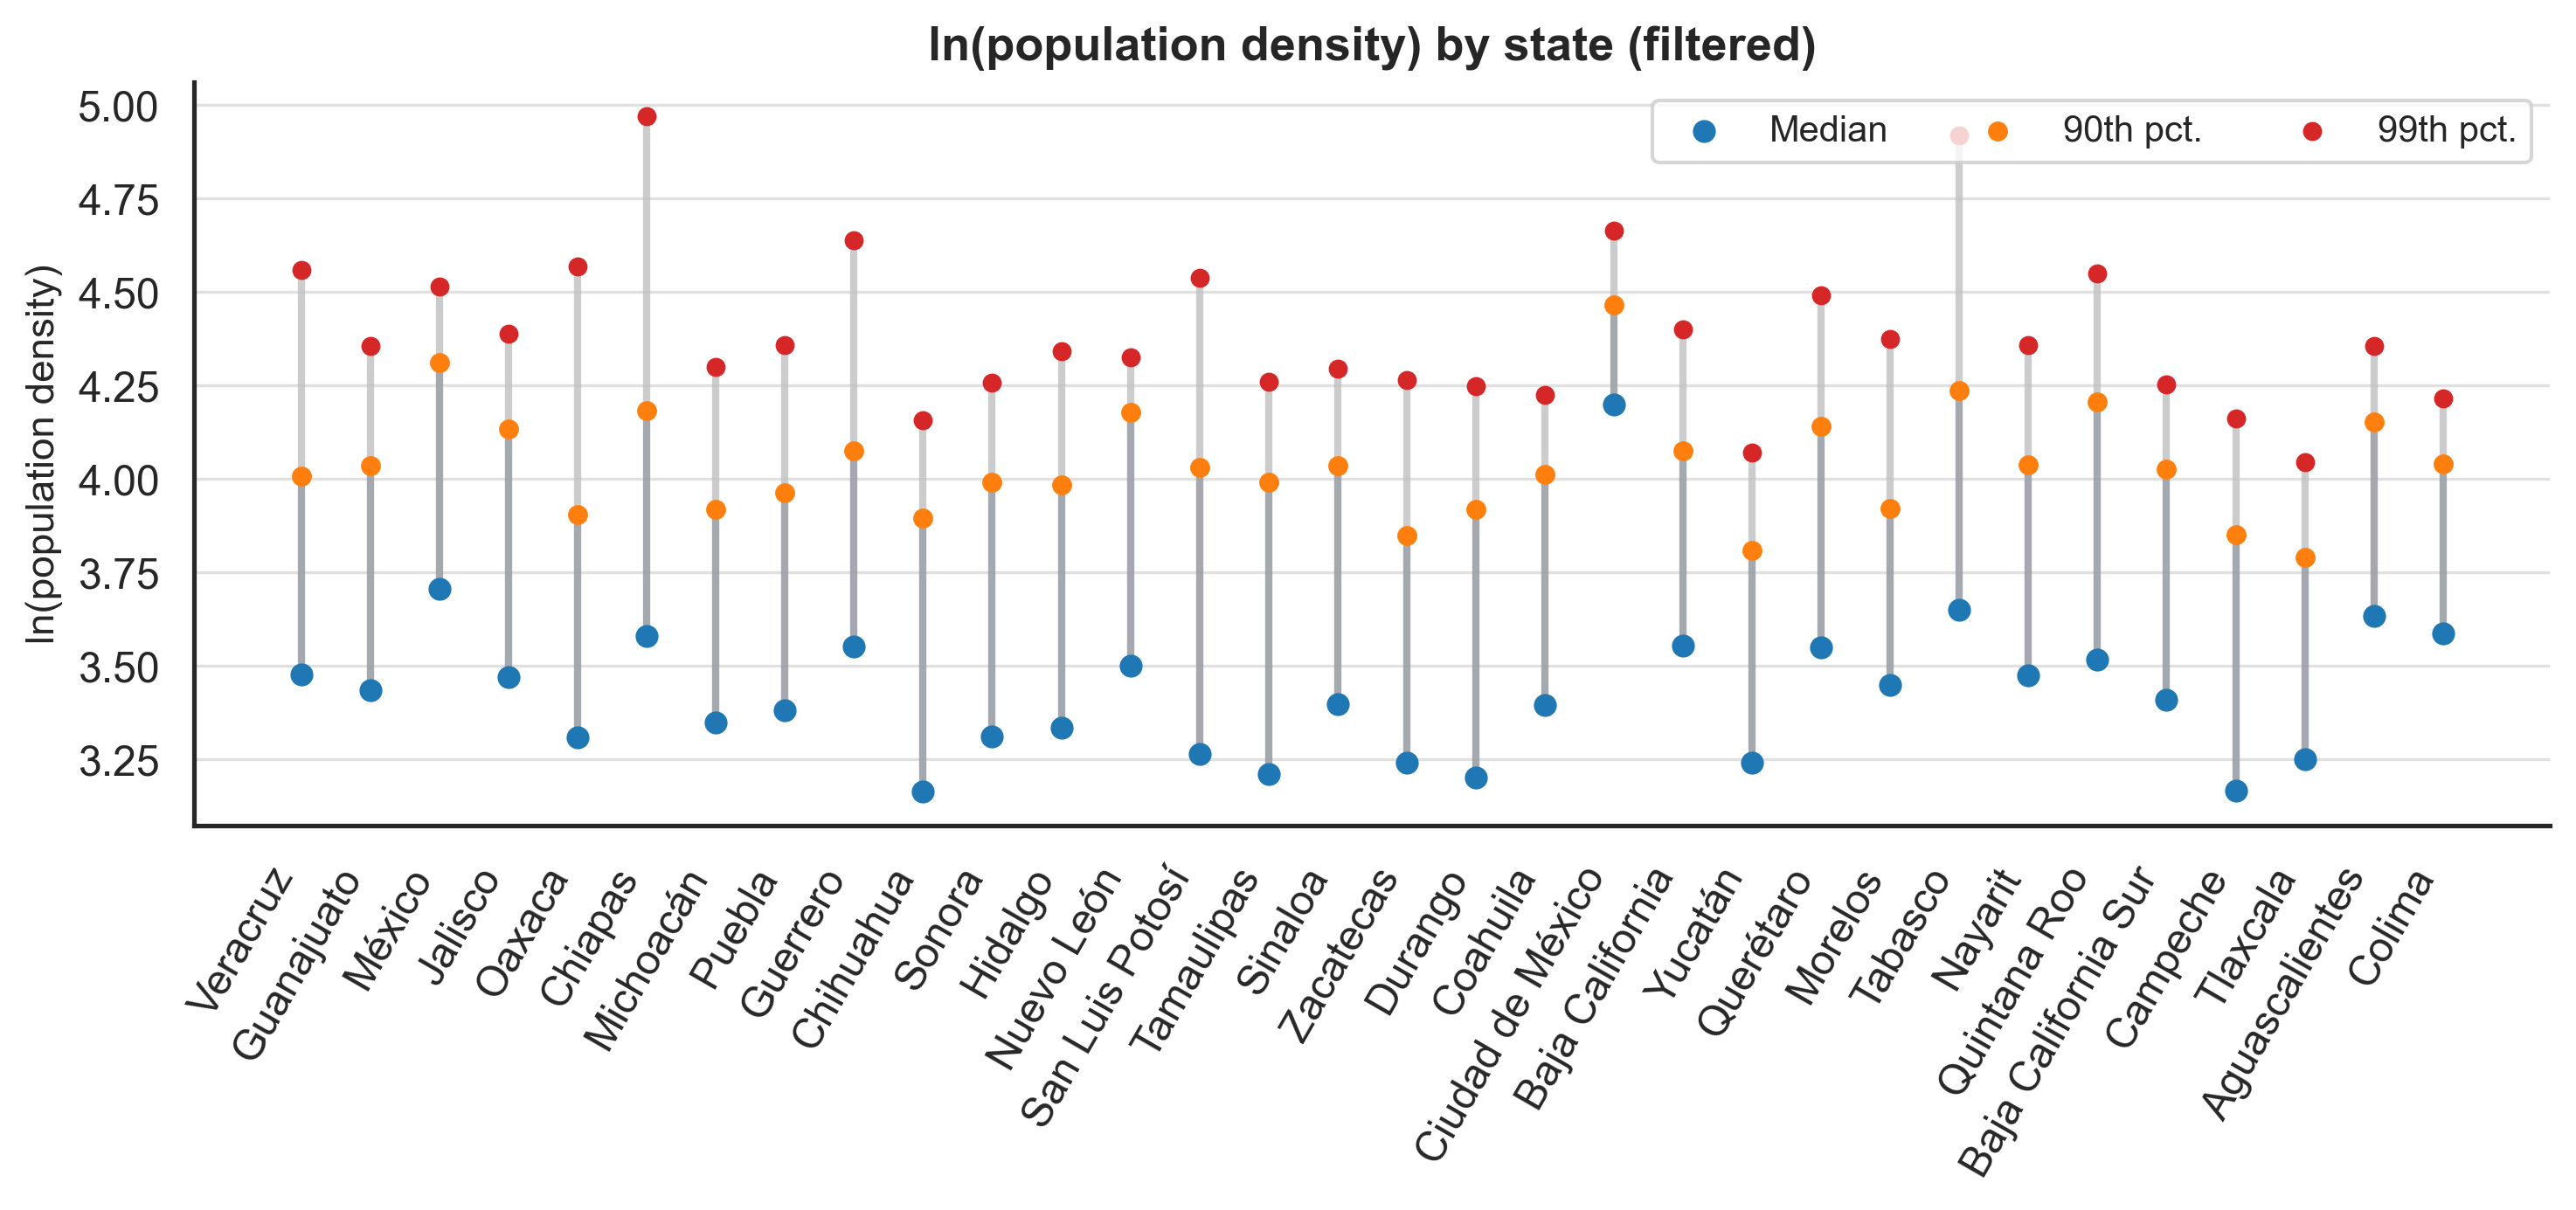
\includegraphics[width=0.8\linewidth]{figs/eda_state_log_popden_quantiles.png}}}
  \caption{ln(population density) by state (filtered): median, 90th percentile, and 99th percentile.}
  \label{fig:eda_state_log_popden_quantiles}
\end{figure}


\subsection{AlphaEarth and Clay foundation models}
\label{subsec:alphaearth_clay}
The AlphaEarth Foundation model and the Clay foundation model (v1.0) for Earth data provided the two sources of the geospatial embeddings for this project. Clay is applied to both 2010 and 2020 census data, while AlphaEarth is only applied to 2020 because its embedding data only stretches back to 2017 \parencite{Brownetal2025}.

\subsubsection{What are Embeddings?}
Vision transformer embeddings encode the physical and structural characteristics of a place as observed from satellite, including impervious surface density, building morphology, road network complexity, vegetation patterns, and spectral signatures of land cover. Formally, an embedding is a low-dimensional numerical vector ($d \in [64, 768]$ for AlphaEarth and Clay in this study) that serves as a compressed latent representation of the high-dimensional raw pixel data. These vectors are learned through self-supervised pretraining on millions of unlabeled satellite tiles, where the models are tasked with reconstructing masked patches or predicting temporal consistency. By solving these auxiliary tasks, the foundation model develops a robust understanding of the Earth's surface. For population estimation, this means that the model automatically distills the visual cues of human settlement (e.g., the texture of rooftops or the geometry of street grids) into a feature space that downstream supervised heads can easily map to demographic counts. This approach bypasses the need for manual feature engineering and enables the transfer of knowledge from global-scale datasets to the specific context of Mexico's census geography.

\subsubsection{Key Model Differences}
\paragraph{Pixel resolution.}
Although both pipelines ingest multispectral satellite imagery, they rely on different missions and therefore different native pixel footprints. AlphaEarth's stack reaches up to roughly \emph{10\,m} sampling where Sentinel-class bands permit it. The Clay workflow implemented here feeds \emph{30\,m} Landsat-7 surface reflectance (and thermal) bands, so each Clay pixel integrates roughly nine AlphaEarth-native pixels on a side before any downstream resampling or aggregation.

\paragraph{Accessing embeddings.}
Another difference pertains to how I accessed the embeddings from each model:
\begin{itemize}
  \item AlphaEarth works through a query-based system. The model's outputs are already stored as an Image Collection on Google Earth Engine, and users can request the embedding value for a geometry (or specific latitude, longitude) and timestamp.

  \item Clay, conversely, has a more decentralized workflow that involves downloading pre-trained weights from HuggingFace\footnote{The weights can be accessed online at this link: \url{https://huggingface.co/made-with-clay/Clay}.} and setting up a PyTorch environment to perform offline inference. Users crop the satellite image into input chips (in this case, $128 \times 128$ pixel patches) that they pass into the Clay model's vision transformer (see Figure \ref{fig:rgb_chips_examples} for what an image chip looks like). These input chips are split into a $16 \times 16$ grid of patches, which are each $8\times 8$ pixels ($8 \times 16 = 128$). For each of these $8 \times 8$ pixel patches---corresponding to roughly $240\times 240$\,m on the ground at Landsat's 30\,m sampling---the model returns a 768-dimensional embedding vector (Figure~\ref{fig:clay_pipeline} diagrams this tensor geometry). The compute responsibility for pre-processing Mexico into annual composites, tiling chips, and batching patches is shifted onto the user.
\end{itemize}


\begin{figure}[htbp]
    \centering
    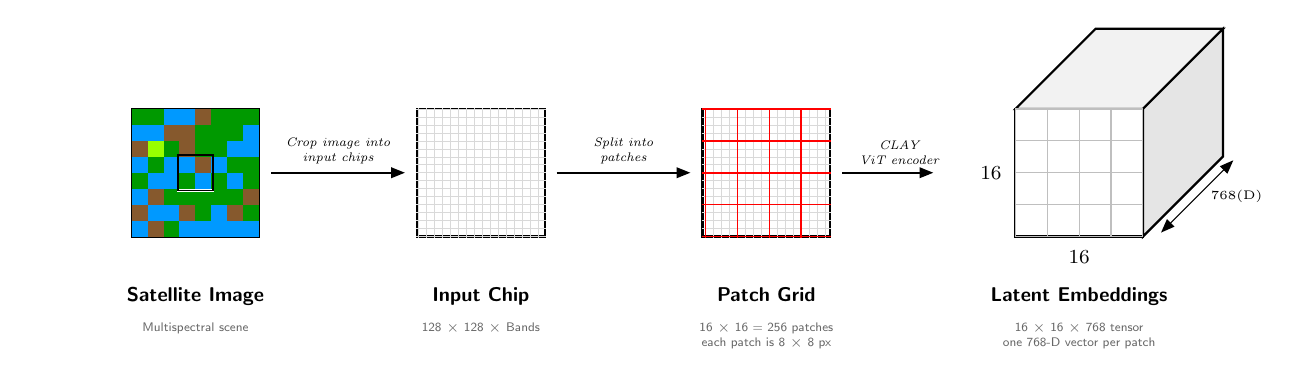
\begin{tikzpicture}[
        scale=0.9, transform shape,
        node distance=2.2cm, 
        font=\sffamily\small,
        >={Stealth[inset=0pt, length=5pt]},
        box/.style={draw, minimum size=1.8cm, thick, fill=white},
        % Increased text width to prevent wrapping
        caption/.style={text width=4cm, align=center, font=\sffamily\footnotesize\bfseries, anchor=north},
        subcaption/.style={text width=4.5cm, align=center, font=\sffamily\tiny, gray!80!black, anchor=north},
        arrow label/.style={midway, above, align=center, font=\tiny\itshape, inner sep=3pt}
    ]

        % --- Coordinates for the baseline alignment ---
        \def\labelY{-1.5cm} 
        \def\subLabelY{-2.0cm} 

        % --- 1. Satellite Image ---
        \node[box] (sat) {};
        \begin{scope}[shift={(sat.center)}]
            \foreach \x in {-0.9,-0.675,...,0.675}
                \foreach \y in {-0.9,-0.675,...,0.675}
                {
                    \pgfmathsetmacro{\randomcolor}{rnd > 0.6 ? "green!60!black" : (rnd > 0.4 ? "blue!40!cyan" : (rnd > 0.2 ? "brown!70!black" : "green!40!yellow"))}
                    \fill[\randomcolor] (\x, \y) rectangle ++(0.225, 0.225);
                }
            \draw[white, thick] (-0.25,-0.25) rectangle (0.25,0.25);
            \draw[black, semithick] (-0.25,-0.25) rectangle (0.25,0.25);
        \end{scope}
        
        \node[caption] at (sat.center |- 0,\labelY) (cap1) {Satellite Image};
        \node[subcaption] at (sat.center |- 0,\subLabelY) {Multispectral scene};

        % --- 2. Input Chip ---
        \node[box, right=of sat] (chip) {};
        \draw[step=0.1125cm, gray!30, very thin] (chip.south west) grid (chip.north east);
        
        \node[caption] at (chip.center |- 0,\labelY) (cap2) {Input Chip};
        \node[subcaption] at (chip.center |- 0,\subLabelY) {128 $\times$ 128 $\times$ Bands};

        % --- 3. Patch Grid ---
        \node[box, right=of chip] (patch) {};
        \draw[step=0.1125cm, gray!30, very thin] (patch.south west) grid (patch.north east);
        \draw[step=0.45cm, red, semithick] (patch.south west) grid (patch.north east);
        
        \node[caption] at (patch.center |- 0,\labelY) (cap3) {Patch Grid};
        \node[subcaption] at (patch.center |- 0,\subLabelY) {16 $\times$ 16 = 256 patches \\ each patch is 8 $\times$ 8 px};

        % --- 4. Latent Embeddings (3D Tensor) ---
        % Pushed slightly further right (2.6cm) to accommodate wider text
        \begin{scope}[shift={($(patch.east)+(2.6cm, -0.9cm)$)}]
            \def\side{1.8}
            \def\depth{1.6} 
            
            \draw[thick, fill=white!95!black] (0,\side) -- ++(45:\depth) coordinate (Dt) -- ++(\side,0) coordinate (Ct) -- (\side,\side) -- cycle;
            \draw[thick, fill=white!90!black] (\side,0) -- ++(45:\depth) coordinate (Bt) -- (Ct) -- (\side,\side) -- cycle;
            \draw[thick, fill=white] (0,0) rectangle (\side,\side);
            \draw[step=0.45cm, gray!50, thin] (0,0) grid (\side,\side);
            
            \draw[<->, shorten >=2pt, shorten <=2pt] (\side+0.2, 0) -- ++(45:\depth) node[midway, right=2pt, font=\tiny] {768(D)};
            \node[left=2pt, font=\footnotesize] at (0, \side/2) {16};
            \node[below=2pt, font=\footnotesize] at (\side/2, 0) {16};
            
            \coordinate (tensor_mid) at (\side/2, 0);
        \end{scope}

        % "Latent Embeddings" now stays on one line
        \node[caption] at (tensor_mid |- 0,\labelY) (cap4) {Latent Embeddings};
        \node[subcaption] at (tensor_mid |- 0,\subLabelY) {16 $\times$ 16 $\times$ 768 tensor \\ one 768-D vector per patch};

        % --- Arrows ---
        \draw[->, thick, shorten >=4pt, shorten <=4pt] (sat.east) -- (chip.west) 
            node[arrow label] {Crop image into \\input chips};
            
        \draw[->, thick, shorten >=4pt, shorten <=4pt] (chip.east) -- (patch.west) 
            node[arrow label] {Split into\\patches};
            
        \draw[->, thick, shorten >=4pt, shorten <=4pt] (patch.east) -- ++(1.6,0) 
            node[arrow label, pos=0.6] {CLAY\\ViT encoder};

    \end{tikzpicture}
    \caption{Data pipeline for the CLAY Vision Transformer model. It showcases how a multispectral scene is cropped, gridded into ViT patches, and mapped to $16\times16\times768$ latent features.}
    \label{fig:clay_pipeline}
\end{figure}


\begin{figure}[H]
  \centering
  \begin{minipage}[t]{0.33\linewidth}
    \centering
    
\includegraphics[width=\linewidth]{figs/chip_180605/inputs/rgb_composite.png}
    \vspace{0.25em}
    {\footnotesize Rural example (\texttt{chip\_180605}).}
  \end{minipage}
  % \hfill
  \begin{minipage}[t]{0.33\linewidth}
    \centering
    
\includegraphics[width=\linewidth]{figs/chip_117931/inputs/rgb_composite.png}
    \vspace{0.25em}
    {\footnotesize Urban example (\texttt{chip\_117931}).}
  \end{minipage}
  \caption{Illustrative RGB input chips (2020) spanning rural and urban contexts. Each panel shows a $128\times128$-pixel input chip extracted from the Landsat-7 imagery stack and rendered as an RGB composite. For visualization, each channel is linearly scaled using a 2nd--98th percentile stretch computed within the chip.}
  \label{fig:rgb_chips_examples}
\end{figure}

Figure~\ref{fig:rgb_chips_examples} shows two representative chips from the 2020 pipeline. The rural chip is dominated by vegetation and bare earth with sparse road structure. The urban chip shows dense rectilinear patterns, bright impenetrable surfaces, and sharp edges. These visual contrasts suggest that raw imagery encodes settlement intensity in ways the encoder can compress into useful features and provides intuition for why foundation-model embeddings can support population-density prediction.

Table~\ref{tab:alphaearth_clay_summary} below summarizes several practical contrasts.

\begin{table}[H]
  \centering
  \caption{Comparison of AlphaEarth Foundation embeddings and Clay (v1.0) for this project}
  \label{tab:alphaearth_clay_summary}
  \renewcommand{\arraystretch}{1.15}
  \setlength{\tabcolsep}{8pt}
  \begin{tabularx}{\linewidth}{@{} l X X @{}}
    \toprule
    \textbf{Feature} & \textbf{AlphaEarth Foundations} & \textbf{Clay (v1.0)} \\
    \midrule
    Architectural unit & Pixel (point-based) & Patch (area-based) \\
    Output dimension & 64-D & 768-D \\
    Primary environment & Google Earth Engine & Python / PyTorch (local/HPC) \\
    Input requirement & Point/polygon coordinates & GeoTIFF image chips ($128 \times 128$) \\
    Compute burden & Managed by Google & Managed by user (GPUs required) \\
    \bottomrule
  \end{tabularx}
\end{table}

\subsubsection{Data Pipelines for Embedding Extraction}

\paragraph{AlphaEarth.}
Since I wrote code to interface with the Google Earth Engine, I could simply load in the AlphaEarth embeddings just by specifying the \texttt{GOOGLE/SATELLITE\_EMBEDDING/\allowbreak V1/ANNUAL} Image Collection for the relevant year and geometries to retrieve data for.

\paragraph{Clay.}
The Clay model, on the other hand, worked locally on my machine and I could not rely on the ease of Google Earth Engine to retrieve the embeddings. Instead, I had to download the cloud-masked composite images for the relevant year and feed them into the Clay model. To create these composites, I processed Landsat-7 (Collection 2, Level 2) imagery for Mexico through a pipeline of radiometric calibration, bitwise quality masking, and temporal aggregation:\footnote{The specific code for this can be found in my project's GitHub repository, which is linked in Section \ref{subsub:computational}.}
\begin{itemize}
  \item Scaled optical and thermal bands using USGS Collection 2 factors ($0.0000275$ gain/$-0.2$ offset and $0.00341802$ gain/$149.0$ offset, respectively) to derive physical surface reflectance and temperature.
  \item Applied an enhanced quality mask via the \texttt{QA\_PIXEL} and \texttt{QA\_RADSAT} bands, utilizing a bitwise AND operation on the first five bits to exclude clouds, shadows, and water while filtering for radiometric saturation.
  \item Applied a temporal median reducer at $30\,\mathrm{m}$ resolution to minimize atmospheric noise and outliers that may appear on an arbitrary day.
\end{itemize}

\paragraph{Landsat continuity (Landsat-7 vs Landsat-8).}
Despite Landsat-8 being launched into orbit in 2013 and thus available to be used for the 2020 datasets, I chose to stick with Landsat-7 (launched in 1999) for the analysis of both 2020 and 2010 census labels to keep consistency across the results. The one drawback of this approach is that I lose out on Landsat-8's enhanced signal-to-noise performance and increased set of bands compared to Landsat-7 (specifically, 12 vs. 8 bands). 



\subsection{Analysis/Prediction Pipeline}

After constructing polygon-level foundation model embeddings, I trained two supervised prediction heads that map embeddings (and a set of geographic covariates) to the target, $\ln(\text{population density})$. The first head is \emph{Ridge regression} (linear least squares with an $\ell_2$ penalty). The second is \emph{XGBoost}, a gradient-boosted ensemble of regression trees. I use both because they offer a transparent linear baseline and a flexible nonlinear alternative while remaining computationally tractable on a hundred thousand polygons.

\subsubsection{Features and Target Variable}
For each polygon $p$, let $y_p$ denote population density (persons per unit area, consistent with the merged census fields) and let $A_p \in \mathbb{R}^{d}$ denote the embedding vector produced by the chosen foundation model after any required aggregation to the polygon. For the AlphaEarth experiments, $d=64$; Clay produces higher-dimensional patch-level representations $d=768$.

To account for state-level heterogeneity (e.g., regional governance, historical development, or cultural settlement drivers) that is not captured by satellite embeddings alone, I include a compact set of state fixed effects via binary indicators. To avoid perfect collinearity with the intercept in the linear ridge model, state $1$ is taken as the omitted category. Let $\mathrm{CVE\_ENT}_p \in \{1,\ldots,32\}$ identify the polygon's state (Mexico's 32 federal entities), the included indicators are thus represented by: $\textbf{1}\{\mathrm{CVE\_ENT}_p=j\}$ for $j=2,\ldots,32$.

The regression target is always the natural log of population density, $\ln y_p$, consistent with the heavy-tailed distributions documented in Section~\ref{subsub:eda}. When reporting fit on the original scale (e.g., for interpretation of errors in ``people per unit area''), predictions are transformed with the exponential map and evaluated alongside the log-scale fit.

\subsubsection{Preprocessing Normalization}
Two normalization steps occur at different stages. First, any radiometric normalization of satellite inputs (e.g., per-band mean/std normalization) is handled upstream by the embedding extraction pipeline before producing $A_p$. Second, for the supervised prediction heads, I standardize the continuous embedding features for ridge regression by z-scoring each embedding dimension using statistics computed on the training split within each cross-validation fold, and then applying the same transform to the held-out fold. XGBoost is trained on the raw feature scales (no standardization), since tree-based splits are not sensitive to linear rescaling of inputs.

Formally, for fold $k$ and feature dimension $j$, let $\mu_{j}^{(k)}$ and $\sigma_{j}^{(k)}$ denote the mean and standard deviation computed on the training split of that fold. The standardized feature is
\[
z_{i j}^{(k)} \;=\; \frac{x_{i j} - \mu_{j}^{(k)}}{\sigma_{j}^{(k)}},
\qquad
\mu_{j}^{(k)}=\frac{1}{n_{\mathrm{train}}}\sum_{i \in \mathrm{train}(k)} x_{i j},
\qquad
\sigma_{j}^{(k)}=\sqrt{\frac{1}{n_{\mathrm{train}}}\sum_{i \in \mathrm{train}(k)}\bigl(x_{i j}-\mu_{j}^{(k)}\bigr)^2}
\]

\subsubsection{Ridge Regression}
\label{subsub:ridge}
Ridge estimates coefficients $(\beta_0,\beta_A,\beta_{\mathrm{ENT}})$ by minimizing penalized squared error,
\[
\sum_{p} \bigl(\ln y_p - \beta_0 - \beta_A^\top A_p - \beta_{\mathrm{ENT}}^\top s_p\bigr)^2 + \alpha \bigl(\lVert \beta_A \rVert_2^2 + \lVert \beta_{\mathrm{ENT}} \rVert_2^2\bigr),
\]
where $s_p$ stacks the state indicators described above and $\alpha>0$ imposes $\ell_2$ shrinkage on all slope coefficients (the intercept $\beta_0$ is unpenalized, following the usual \texttt{Ridge} specification in scikit-learn). Equivalently, the fitted model can be written as
\begin{equation}
\label{eq:ridge_prediction_head}
\ln y_p
  = \beta_0
  + \sum_{i=0}^{d-1} \beta_{A,i}\, A_{p,i}
  + \sum_{j=2}^{32} \beta_{\mathrm{ENT},j}\,\textbf{1}\{\mathrm{CVE\_ENT}_p=j\}
  + \varepsilon_p .
\end{equation}

Note that the $\ell_2$ regularization is used to manage the multicollinearity inherent in the embedding dimensions, which would otherwise lead to unstable OLS estimates with high variance.

\subsubsection{XGBoost (eXtreme Gradient Boosting)}
\label{subsub:xgboost}
XGBoost represents a complementary nonlinear head. Rather than a single linear functional form, it approximates $\ln y_p$ with an additive ensemble of $K$ shallow regression trees $\{f_k\}_{k=1}^{K}$,
\begin{equation}
\label{eq:xgb_prediction_head}
\ln y_p
  = \sum_{k=1}^{K} f_k\bigl(A_{p,0},\ldots,A_{p,d-1},\,\textbf{1}\{\mathrm{CVE\_ENT}_p=2\},\ldots,\textbf{1}\{\mathrm{CVE\_ENT}_p=32\}\bigr) + \varepsilon_p ,
\end{equation}
where each $f_k$ is a weak learner constrained by tree depth, row subsampling, and column subsampling to reduce variance. In practice, the same state indicators enter the tree model as additional binary splits alongside the continuous embedding coordinates, allowing interactions between spectral structure and broad geography without hand-specifying feature crosses.

\subsubsection{Hyperparameter Tuning}
Hyperparameter optimization is essential for calibrating the complexity of the regression heads against the high-dimensional feature space provided by the embeddings. I tuned as follows:

\paragraph{Clay.} Ridge regression used grid search over the regularization strength $\alpha$; XGBoost used random search with 100 trials over continuous ranges. The full search spaces and strategies are listed in Table~\ref{tab:hyperparameters} in Appendix~\ref{app:hyperparameters}.

\paragraph{AlphaEarth.} Ridge regression used randomized search with 40 trials over the regularization strength $\alpha$; XGBoost used randomized search with 30 trials over a discrete hyperparameter grid; both used 3-fold cross-validation (mean $R^2$). The full search spaces and strategies are listed in Table~\ref{tab:hyperparameters_alphaearth} in Appendix~\ref{app:hyperparameters}.

Table~\ref{tab:final_parameters} reports the best hyperparameters selected under 5-fold cross-validation  on log population density, shown separately for the 2010 and 2020 training configurations.

\begin{table}[H]
  \centering
  \caption{Best-tuned prediction-head hyperparameters by census year (5-fold CV, seed 0, embedding-only feature set). Floating-point entries are rounded to four decimal places.}
  \label{tab:final_parameters}
  \renewcommand{\arraystretch}{1.12}
  \setlength{\tabcolsep}{10pt}
  \begin{tabular}{@{}l ccc@{}}
    \toprule
    \textbf{Parameter} & \textbf{2010 (Clay)} & \textbf{2020 (Clay)} & \textbf{2020 (AlphaEarth)} \\
    \midrule
    \multicolumn{4}{@{}l}{\textbf{Ridge}} \\
    $\alpha$ & 1000 & 1000 & 17.8984 \\
    \midrule
    \multicolumn{4}{@{}l}{\textbf{XGBoost}} \\
    Learning rate ($\eta$) & 0.0361 & 0.0396 & 0.1000 \\
    Max depth & 5 & 7 & 8 \\
    Subsample & 0.7695 & 0.9020 & 1.0000 \\
    \texttt{colsample\_bytree} & 0.8345 & 0.7941 & 0.7000 \\
    \texttt{reg\_lambda} ($\lambda$) & 0.0041 & 3.4955 & 5.0000 \\
    \texttt{reg\_alpha} ($\alpha$) & 5.4334 & 0.0186 & 0.1000 \\
    \texttt{min\_child\_weight} & 7.0183 & 25.2185 & 7 \\
    $\gamma$ & 1.3149 & 0.0021 & 0 \\
    \midrule
    \multicolumn{4}{@{}l}{\textbf{Fixed (both years)}} \\
    \texttt{n\_estimators} & 2000 & 2000 & 1200 \\
    Early stopping (rounds) & 50 & 50 & --- \\
    \bottomrule
  \end{tabular}
\end{table}

\subsubsection{Evaluation Strategy}
\label{subsub:eval_strategy}

The empirical scores reported in this thesis come from a common evaluation harness that fits the prediction heads and computes out-of-sample metrics under cross-validation.

\paragraph{Evaluation metrics.} I report four standard regression metrics, always computed by comparing predictions $\hat{y}$ to the corresponding realized targets $y$:
\begin{table}[H]
  \centering
  \caption{Evaluation metrics used throughout the analysis.}
  \label{tab:eval_metrics_code}
  \renewcommand{\arraystretch}{2.2}
  \setlength{\tabcolsep}{10pt}
  \begin{tabular}{@{}ll@{}}
    \toprule
    \textbf{Metric} & \textbf{Definition} \\
    \midrule
    $R^2$ (coefficient of determination) &
    $1 - \dfrac{\sum_{i=1}^{n} (y_i - \hat{y}_i)^2}{\sum_{i=1}^{n} (y_i - \bar{y})^2}$ \\
    Pearson $r$ (correlation coefficient) & 
    $\dfrac{\sum_{i=1}^{n} (y_i - \bar{y})(\hat{y}_i - \bar{\hat{y}})}{\sqrt{\sum_{i=1}^{n} (y_i - \bar{y})^2} \sqrt{\sum_{i=1}^{n} (\hat{y}_i - \bar{\hat{y}})^2}}$ \\
    MAE (mean absolute error) &
    $\dfrac{1}{n}\sum_{i=1}^{n} \lvert y_i - \hat{y}_i \rvert$ \\
    RMSE (root mean squared error) &
    $\sqrt{\dfrac{1}{n}\sum_{i=1}^{n} (y_i - \hat{y}_i)^2}$ \\
    \bottomrule
  \end{tabular}
\end{table}

\paragraph{Target scale.} Unless noted otherwise, the target is \texttt{log\_popden} (natural log of population density). MAE and RMSE are therefore reported in log units unless predictions are explicitly inverse-transformed. To inverse-transform, I used an exponential map: $\exp(\hat{y})$.

Thus, $R^2_{\ln}$ is evaluated on the scale actually used in training and therefore captures whether embeddings organize variation in log density itself. $R^2_{\mathrm{orig}}$ offers an intuitive link to people-per-unit-area outcomes but can be dominated by a minority of extremely dense polygons and should always be read together with $R^2_{\ln}$, not in isolation.

\paragraph{Cross-validation and out-of-fold prediction.} Reported scores are out-of-fold (OOF), meaning each row's prediction is generated by a model that did not train on that row. Specifically, I default to using a shuffled $K$-fold cross-validation, with $K=5$.

Figure~\ref{fig:fold_map_cdmx} visualizes the shuffled 5-fold assignment for urban AGEBs in Mexico City. Since folds are assigned randomly at the polygon level, nearby neighborhoods are typically interleaved across folds rather than forming contiguous uniform blocks. This illustrates why shuffled $K$-fold is best interpreted as a general out-of-sample check under the observed spatial mix.

\begin{figure}[H]
  \centering
  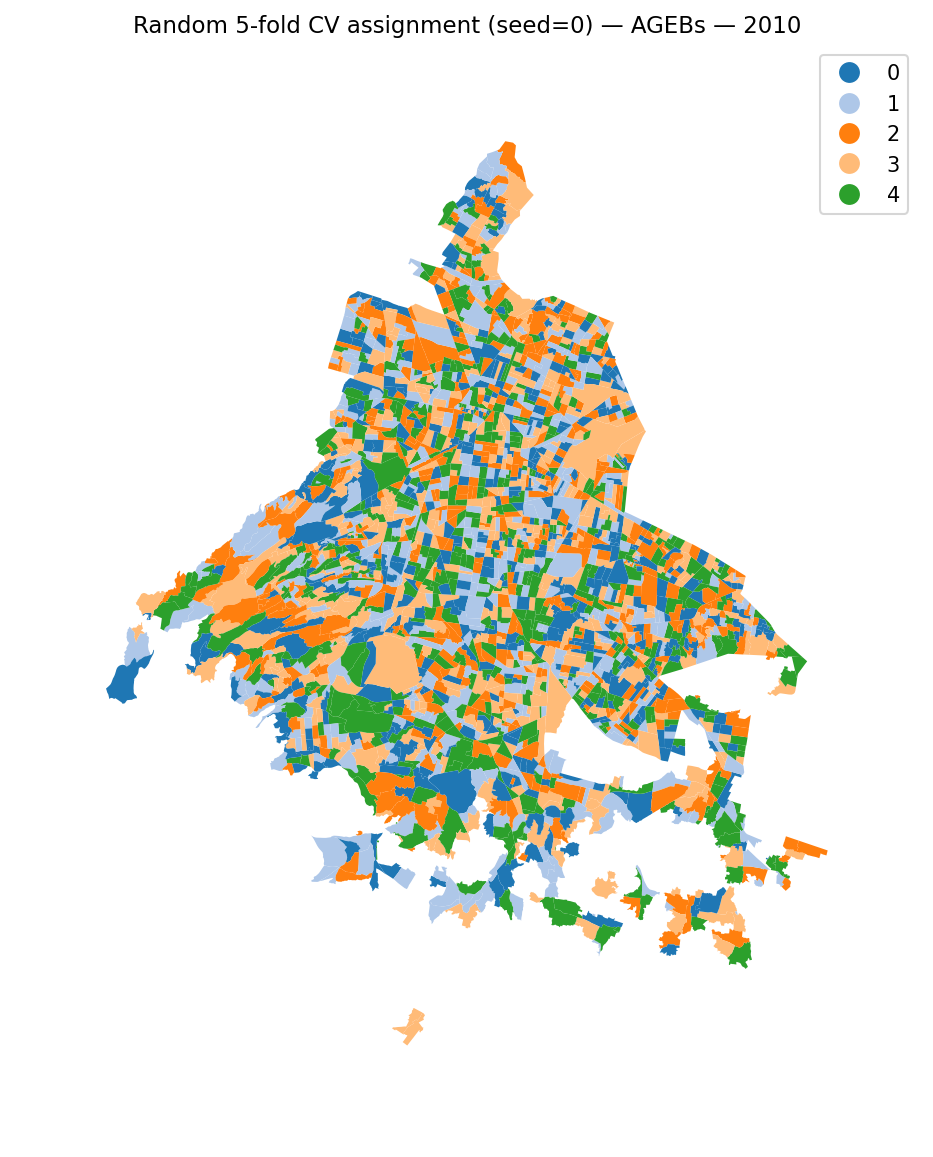
\includegraphics[width=0.45\linewidth]{figs/fold_map_cdmx.png}
  \caption{Example fold map for shuffled 5-fold cross-validation (seed 0) on urban AGEBs in Mexico City (CDMX), 2010. Colors indicate fold membership; the patchwork pattern reflects random assignment at the polygon level (folds are geographically interspersed rather than spatially contiguous).}
  \label{fig:fold_map_cdmx}
\end{figure}

\paragraph{Spatial units evaluated.} The same evaluation code is run at multiple spatial resolutions. The key difference between the two \emph{municipio} constructions is that \emph{rollup} aggregates from labeled AGEB polygons up to municipalities, while \emph{direct} aggregates from the embedding cell grid into municipality footprints. There are 2469 municipalities for 2020 census data and 2456 for 2010 census data (i.e., 13 municipalities were added in the decade). 
\begin{itemize}
  \item \textbf{AGEB}: polygon-level features and targets
  \item \textbf{\emph{Municipio} (rollup)}: municipality features formed by aggregating AGEB polygons. Each AGEB is assigned to a \emph{municipio} by the first five digits of \texttt{CVEGEO} (two-digit state + three-digit \emph{municipio}). Embeddings are aggregated to the municipality via an area-weighted mean across AGEBs, and municipality-level targets are recomputed by summing population and land area across constituent AGEBs before taking density.
  \item \textbf{\emph{Municipio} (direct)}: municipality features extracted directly from the embedding grid rather than from AGEB summaries. AGEB polygons are first dissolved into municipality footprints, then embedding cells are assigned to municipalities using centroid-in-polygon logic; municipality embeddings are computed by aggregating the assigned cells (and targets are computed at the municipality scale using the dissolved geometry / summed population and area).
\end{itemize}

\subsubsection{Overview of Empirical Experiments}
\label{subsec:experiment-overview}

This project organizes supervised runs that reuse the same ridge and XGBoost heads but vary the embedding source, label census year, spatial aggregation, and (for Clay) temporal linkage between 2010 and 2020. Table~\ref{tab:experiment_overview} lays out a guide to the empirical experiments run. It avoids numeric scores (those appear in the Section \ref{sec:results} tables and figures) and instead states what each family of runs is trying to isolate.

\begin{table}[H]
  \centering
  \caption{Road map of empirical experiments. ``OOF'' denotes out-of-fold prediction under the project's default five-fold cross-validation scheme.}
  \label{tab:experiment_overview}
  \footnotesize
  \renewcommand{\arraystretch}{1.2}
  \setlength{\tabcolsep}{5pt}
  \begin{tabular}{@{} >{\raggedright\arraybackslash}p{0.18\textwidth} >{\raggedright\arraybackslash}p{0.28\textwidth} >{\raggedright\arraybackslash}p{0.22\textwidth} >{\raggedright\arraybackslash}p{0.28\textwidth} @{}}
    \toprule
    \textbf{Experiment family} & 
    \textbf{Embedding / outcome pairing} & 
    \textbf{Spatial resolution} & 
    \textbf{Purpose \& where it appears} \\
    \midrule
    Cross-sectional benchmarking & 
    AlphaEarth (2020); Clay (2020); and Clay (2010). All paired with contemporaneous census labels. & 
    Urban AGEB and rural locality polygons; municipality aggregates via area-weighted rollup. & 
    Primary performance comparison: $R^2$ and MAE benchmarks (Table~\ref{tab:results_embedding_comparison}) and graphical calibration/residual diagnostics (Figure~\ref{fig:oof_calibration_all}). \\
    \addlinespace[3pt]
    Spatial heterogeneity \& drivers & 
    Same cross-sectional setups as above. & 
    Polygon scale; metrics summarized by state ($n=32$). & 
    Mapping performance variance (Figure~\ref{fig:spatial_state_r2}) and identifying statistical drivers ($r$) such as polygon area and target variance (Table~\ref{tab:avgcharacteristics}). \\
    \addlinespace[3pt]
    Systematic prediction bias & 
    Same cross-sectional setups as above. & 
    State-level mean of residuals ($\bar{e}_s$). & 
    Identifying persistent geographic over- or under-prediction based on land-cover or regional traits (Figure~\ref{fig:spatial_state_bias}). \\
    \addlinespace[3pt]
    Cross-decadal temporal linkage & 
    2010 embeddings $\to$ 2020 labels; $[\mathrm{emb}_{2010}, \Delta\mathrm{emb}]$ features; and full 2010-to-2020 transfer. & 
    Matched panel of AGEB intersections (2010--2020) and full 2020 grid. & 
    Testing temporal signal and change detection: prediction levels (Table~\ref{tab:clay_temporal_cross_year}) and directional accuracy for decadal growth ($\Delta\ln y$) (Figure~\ref{fig:temporal_change_cross_temporal}). \\
    \bottomrule
  \end{tabular}

  \medskip
  \raggedright
  \textit{Notes:} Diagnostic figures and state-level analyses reuse the underlying OOF prediction tables generated during the benchmarking phase and do not involve separate training stages.
\end{table}

\subsubsection{Computational Environment}
\label{subsub:computational}

\paragraph{Google Earth Engine.} For AlphaEarth, I wrote JavaScript scripts in the Google Earth Engine Code Editor (web interface) to build cloud composites over the study imagery and drive extraction of AlphaEarth Foundations embeddings on Google's hosted stack, exporting tile-level vectors for later merger with census geometries.

\paragraph{Software stack (Python).} Downstream supervised modeling and evaluation---ridge and XGBoost heads, randomized hyperparameter search, $K$-fold cross-validation, and municipality rollups---were implemented in Python~3 using \texttt{conda}-style environments on the cluster and locally. Core libraries included \texttt{numpy} and \texttt{pandas} for tabular data; \texttt{scikit-learn} for pipelines, \texttt{Ridge}, \texttt{StandardScaler}, cross-validation, and metrics; \texttt{scipy} for sampling distributions in search; \texttt{xgboost} for gradient-boosted trees; and \texttt{joblib} for persisting fitted models. Clay encoder inference used \texttt{torch} with CUDA together with the Clay model codebase as released by Radiant Earth; exploratory analysis and figure generation used \texttt{jupyter} notebooks. Tabular merges and all regression experiments that consumed AlphaEarth embeddings began from the Earth Engine exports described above.

\paragraph{Hardware and scheduling.} Computationally intensive steps (especially applying foundation-model encoders over large stacks of satellite tiles) were run on Yale Research Computing's Bouchet cluster. Jobs were submitted with SLURM (\texttt{sbatch}). Clay embedding extraction used the GPU partition with CUDA-capable NVIDIA GPUs. Auxiliary cluster tasks that did not require inference (for example spatial aggregation of cell embeddings to census polygons) ran on CPU nodes in the same environment.

\paragraph{Code availability.} To support the reproducibility of this thesis, all source code for the AlphaEarth and Clay foundation model pipelines---including scripts for Google Earth Engine data preparation, model training, evaluation, and figure generation---is available on GitHub at \url{https://github.com/henryjchen/cs-econ-thesis}. Please reach out to \href{mailto:henry.chen@yale.edu}{henry.chen@yale.edu} if you have any questions.


\newpage

\section{Results}
\label{sec:results}

This section presents the empirical findings from the aforementioned experiments (Section \ref{subsec:experiment-overview}). It presents scalar benchmark scores across embeddings and spatial scales; graphical calibration checks, regional error patterns at the state level, and Clay-specific temporal experiments linking the 2010 encoder to 2020 labels and decadal change on matched polygons. Unless noted otherwise, every prediction is done out-of-fold.


\subsection{Out-of-Fold Prediction Performance}

Table~\ref{tab:results_embedding_comparison} helps answer our first research question (Section \ref{sub:researchque}) by showing how much cross-sectional variation in population density Ridge regression and XGBoost can explain across AlphaEarth and Clay embeddings. Ridge regression and XGBoost are run with the specifications from Section \ref{subsub:ridge} and \ref{subsub:xgboost}, respectively.

\begin{table}[H]
  \centering
  \caption{Out-of-fold regression metrics by embedding source and census year. Columns give $R^2$ on the $\ln(\text{population density})$ target and on the inverse-transformed density scale at polygon resolution (urban AGEB / rural locality) and after municipality aggregation using the roll-up methodology (see Section \ref{subsub:eval_strategy}).}
  \label{tab:results_embedding_comparison}
  \footnotesize
  \renewcommand{\arraystretch}{1.15}
  \setlength{\tabcolsep}{5pt}
  \begin{tabular}{@{} l l cccc @{}}
    \toprule
    \textbf{Embedding setup} & \textbf{Head} & 
    \multicolumn{2}{c}{\textbf{Polygon level (AGEB and localities)}} & 
    \multicolumn{2}{c}{\textbf{Municipality level}} \\
    \cmidrule(lr){3-4}\cmidrule(lr){5-6}
    & & $R^2_{\ln}$ & $R^2_{\mathrm{orig}}$ & $R^2_{\ln}$ & $R^2_{\mathrm{orig}}$ \\
    \midrule
    AlphaEarth (2020 labels) & Ridge    & 0.629 & 0.589 & 0.691 & 0.757 \\
                             & XGBoost  & \cellcolor{teal!15}{0.727} & \cellcolor{teal!15}{0.701} & \cellcolor{teal!15}{0.879} & \cellcolor{teal!15}{0.898} \\
    \addlinespace[2pt]
    Clay (2020 labels)       & Ridge    & 0.513 & 0.118 & 0.644 & 0.415 \\
                             & XGBoost  & 0.609 & 0.169 & 0.749 & 0.753 \\
    \addlinespace[2pt]
    Clay (2010 labels)       & Ridge    & 0.581 & 0.529 & 0.631 & 0.426 \\
                             & XGBoost  & 0.629 & 0.654 & 0.725 & 0.748 \\
    \bottomrule
  \end{tabular}

  \medskip
  \raggedright
  \textit{Notes:} $R^2_{\ln}$ is computed on the fitted $\ln(\text{population density})$ target. $R^2_{\mathrm{orig}}$ maps OOF predictions and truth to the density scale via naive exponentiation. \colorbox{teal!15}{highlighted} cells mark the column-best $R^2$.
\end{table}


AlphaEarth attains the strongest polygon-scale scores in the table for both prediction heads. Clay with 2020 imagery trails materially at the polygon level---particularly on Ridge's linear-scale $R^2_{\mathrm{orig}}$---yet narrows part of the gap once predictions aggregate to the municipality level. This is consistent with noise averaging across coarse geography. 

Clay paired with 2010 labels performs better than Clay with 2020 labels but worse than AlphaEarth at the polygon level. This suggests that the more uniform training / evaluation set of 2010 (which is just urban AGEBs and does not include rural locality points) might make it easier for the model to perform at the most granular levels. Despite this, Clay 2020 outperforms Clay 2010 at the municipality level, likely because municipalities include both AGEB and localities, so the 2010 set not including locality data will overlook this aspect of the municipality's characteristics.



\subsubsection{Case Studies}
\label{sub:case_studies}

To move beyond aggregate metrics, we visualize polygon-level predictions for three high-performing municipalities whose urban forms span a range of Mexican city types: \emph{Monterrey} (a large industrial metro in Nuevo León), \emph{Querétaro} (a mid-size secondary city undergoing rapid expansion), and \emph{Cancún} (a coastal tourism hub in Quintana Roo). Figure~\ref{fig:case_study_cs} maps actual versus predicted $\ln(\text{population density})$ at the AGEB level using the best-performing cross-sectional specification (AlphaEarth 2020, XGBoost).

\begin{figure}[htbp]
  \centering
  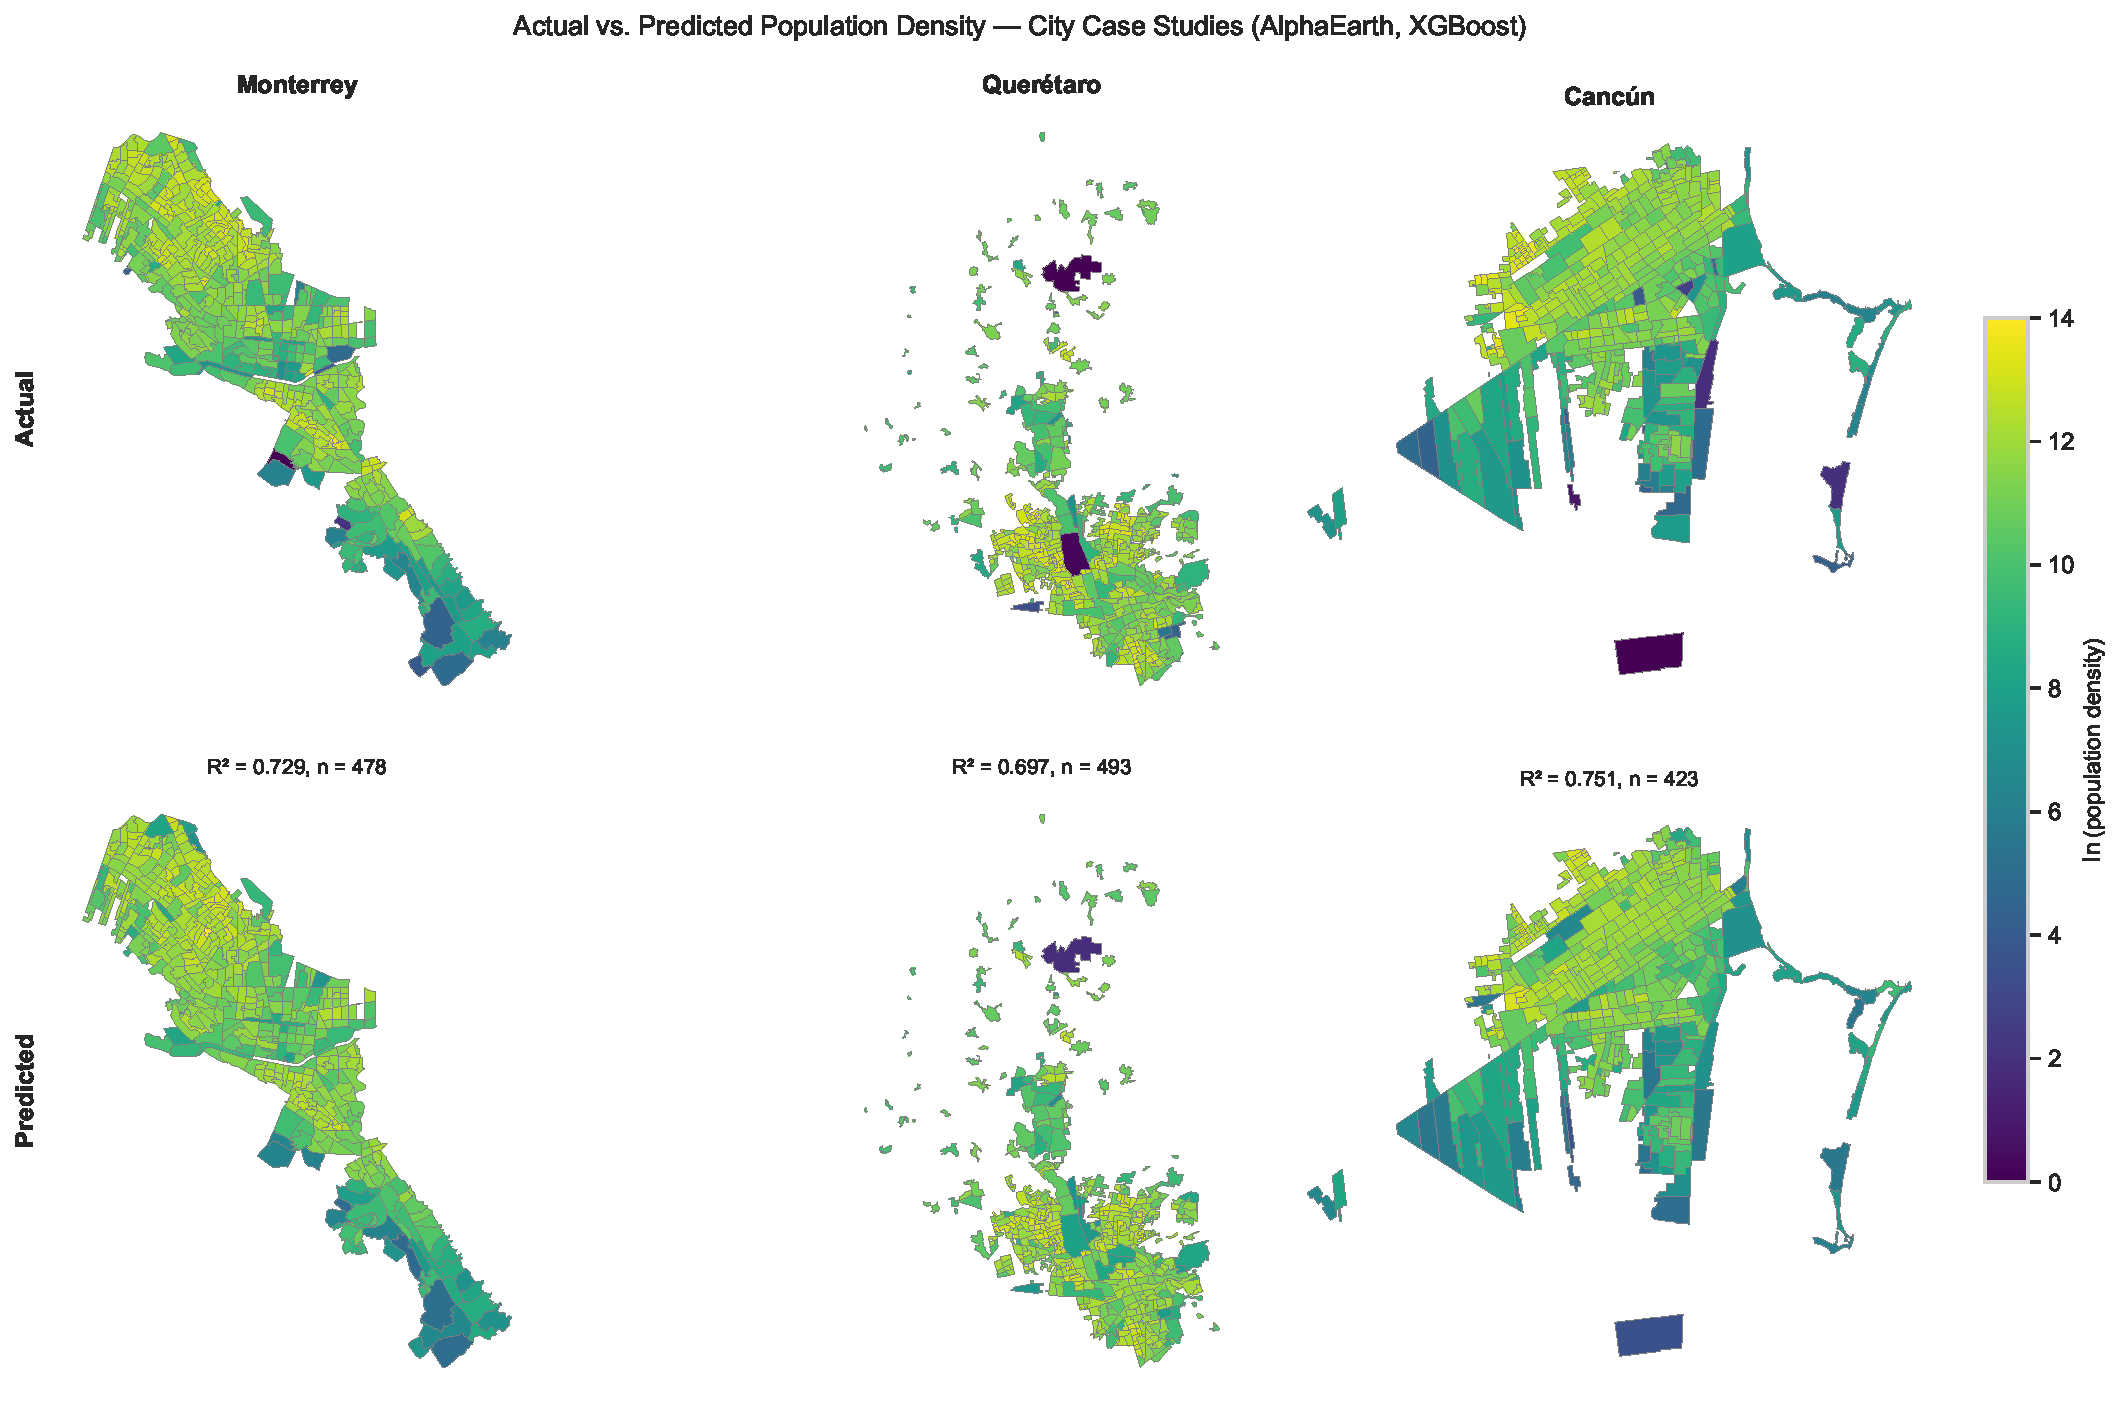
\includegraphics[width=\textwidth]{figs/case_study_actual_vs_predicted.pdf}
  \caption{Actual (top row) versus predicted (bottom row) $\ln(\text{population density})$ for the municipalities of Monterrey, Querétaro, and Cancún. Color encodes $\ln(\text{pop.\ density})$ on a shared viridis scale (0--14). Statistics report within-municipality $R^2$ and sample size. 2020 census data. Color scale shows log population density.}
  \label{fig:case_study_cs}
\end{figure}

Across all three cities the model reproduces the broad intra-urban density gradient---high-density residential cores appear in yellow-green, while peripheral and industrial zones transition to darker blue-green---with close visual correspondence between the actual and predicted maps. Monterrey ($R^2 = 0.729$, $n = 478$) displays the characteristic north--south density spine of its metropolitan corridor, which the model captures faithfully despite considerable morphological heterogeneity between the dense center and the sprawling southern suburbs. Querétaro ($R^2 = 0.697$, $n = 493$) presents a radial density decay from its colonial core; the predicted map correctly identifies the low-density industrial parks ringing the city as well as the denser satellite neighborhoods to the south. Cancún ($R^2 = 0.751$, $n = 423$) is perhaps the most visually striking match. The model is able to distinguish the high-density hotel zone peninsula from the lower-density residential grid to the west and the near-empty lagoon parcels, suggesting that AlphaEarth embeddings encode fine-grained land-cover cues (like built-up shoreline vs. mangrove) that translate directly into density predictions.

These case studies illustrate that the aggregate $R^2$ values reported in Table~\ref{tab:results_embedding_comparison} are not driven solely by between-state variation; the foundation model embeddings contain sufficient spatial information to recover density patterns \emph{within} individual cities, across a range of urban morphologies and climatic zones.

\subsubsection{Calibration and Residual Diagnostics}
\label{sub:calibration_diagnostics}

The above $R^2$ scores were calculated in aggregate and compresses all the deviations into one ratio. To get a better sense of where predictions lie relative to truth at polygon scale for each embedding setup we plot the following diagnostics (Figures~\ref{fig:oof_alphaearth2020}--\ref{fig:oof_clay2010}). 

In each figure pair, the upper panels display realized $\ln(y)$ vs. predicted $\ln(\hat{y})$ with density-coded hexbins (darker cells mean more held-out polygons fall in that bin) and a dashed identity $y=x$ line that represents perfect calibration in log space on cross-validation folds. 

The lower panels, show the distribution of the residuals $\ln(y) - \ln(\hat{y})$ as a probability density, normalized to 1, and overlaid with a Gaussian distribution centered at 0 with standard deviation equal to the sample standard deviation of the residuals that serves as a visual benchmark for the distribution of the residuals. 


The figures suggest that top-level performance gaps across embedding sources reflect systematic calibration differences rather than a handful of extreme outliers alone. AlphaEarth panels exhibit the tightest clustering along the identity line for both heads and residuals concentrated sharply near zero, aligning with Table~\ref{tab:results_embedding_comparison}'s advantage at polygons. Clay (2020) spreads mass farther from the diagonal under ridge and develops thicker residual tails. Clay (2010) reflects an intermediate.



\begin{figure}[H]
  \centering
  % --- Row 1: AlphaEarth (left) and Clay 2020 (right) ---
  \begin{subfigure}[t]{0.50\linewidth}
    \centering
    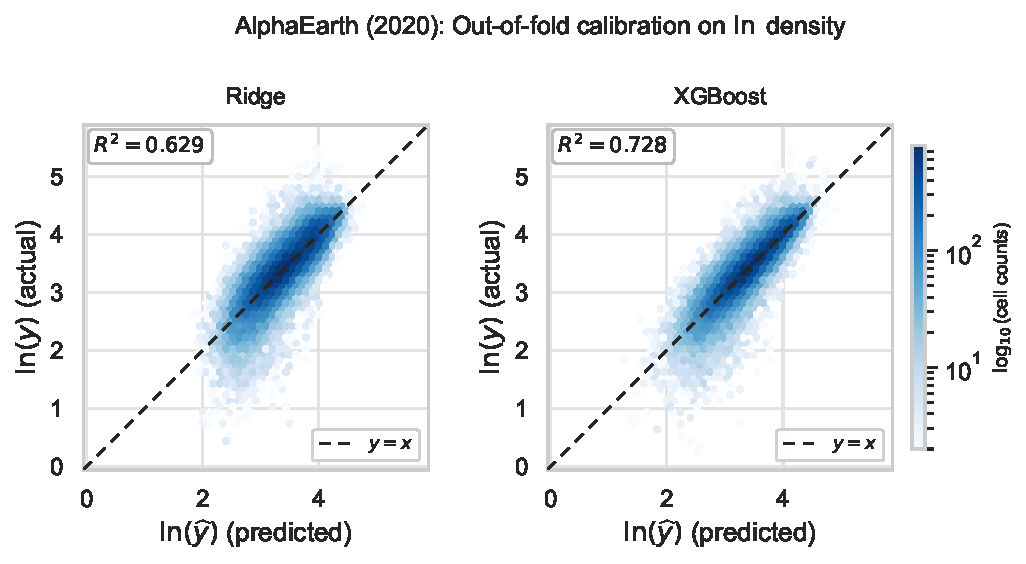
\includegraphics[width=\linewidth]{figs/oof_calibration_alphaearth2020.pdf}\\[0.4em]
    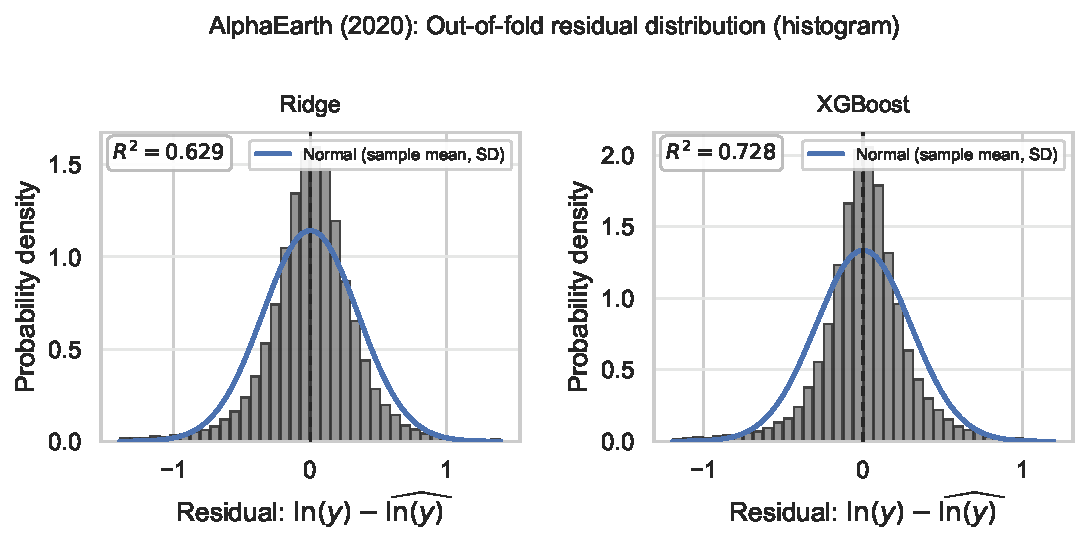
\includegraphics[width=\linewidth]{figs/oof_residuals_alphaearth2020.pdf}
    \caption{AlphaEarth (2020 labels)}
    \label{fig:oof_alphaearth2020}
  \end{subfigure}\hfill
  \begin{subfigure}[t]{0.50\linewidth}
    \centering
    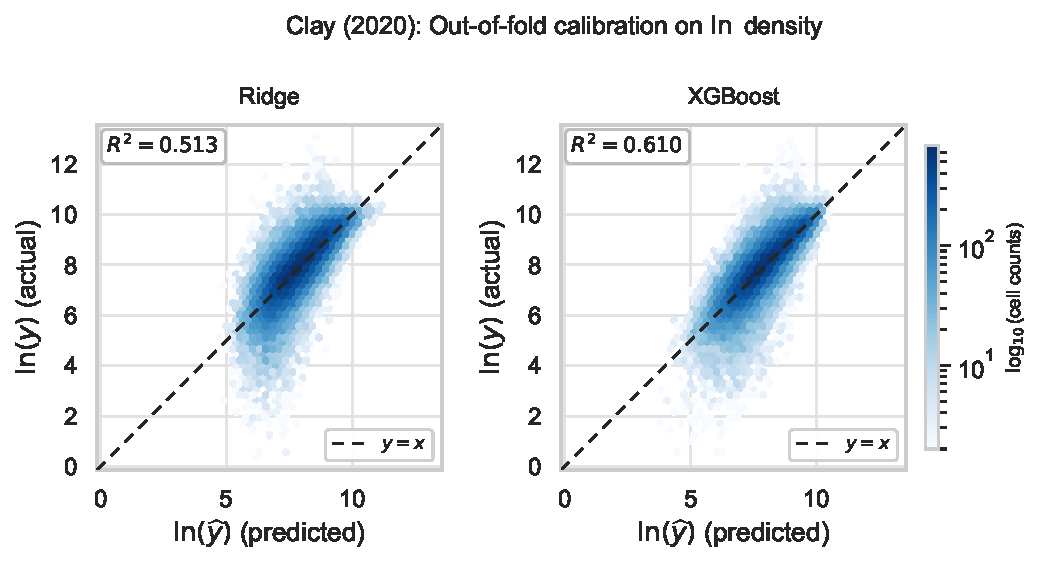
\includegraphics[width=\linewidth]{figs/oof_calibration_clay2020.pdf}\\[0.4em]
    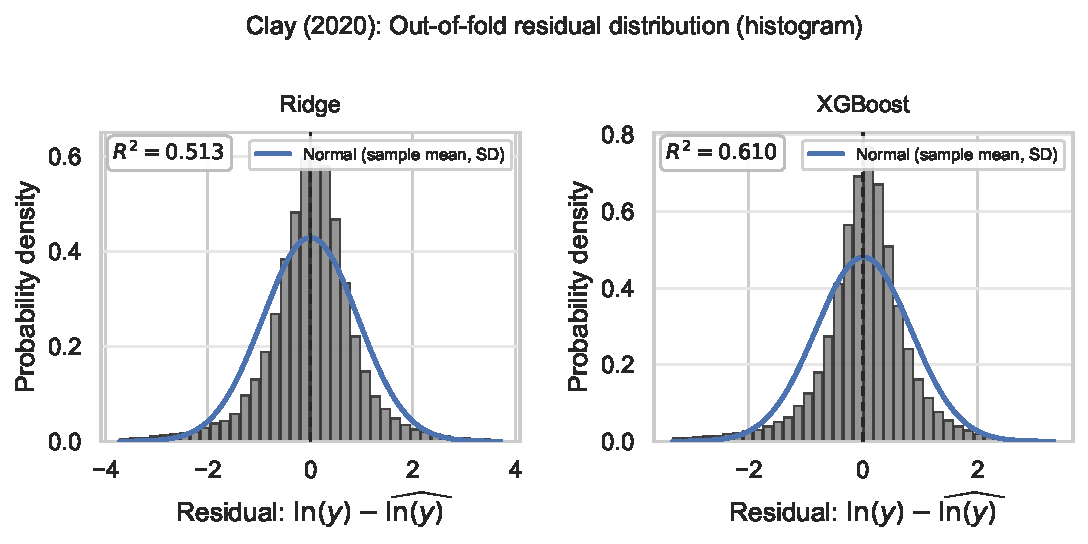
\includegraphics[width=\linewidth]{figs/oof_residuals_clay2020.pdf}
    \caption{Clay (2020 labels)}
    \label{fig:oof_clay2020}
  \end{subfigure}

  \vspace{0.8em}

  % --- Row 2: Clay 2010 (centered) ---
  \begin{subfigure}[t]{0.50\linewidth}
    \centering
    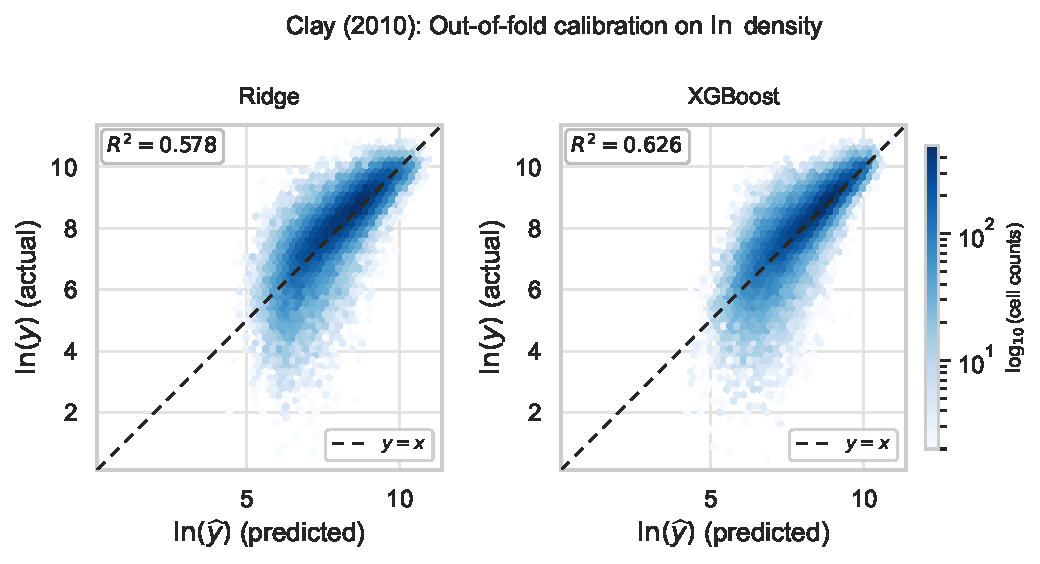
\includegraphics[width=\linewidth]{figs/oof_calibration_clay2010.pdf}\\[0.4em]
    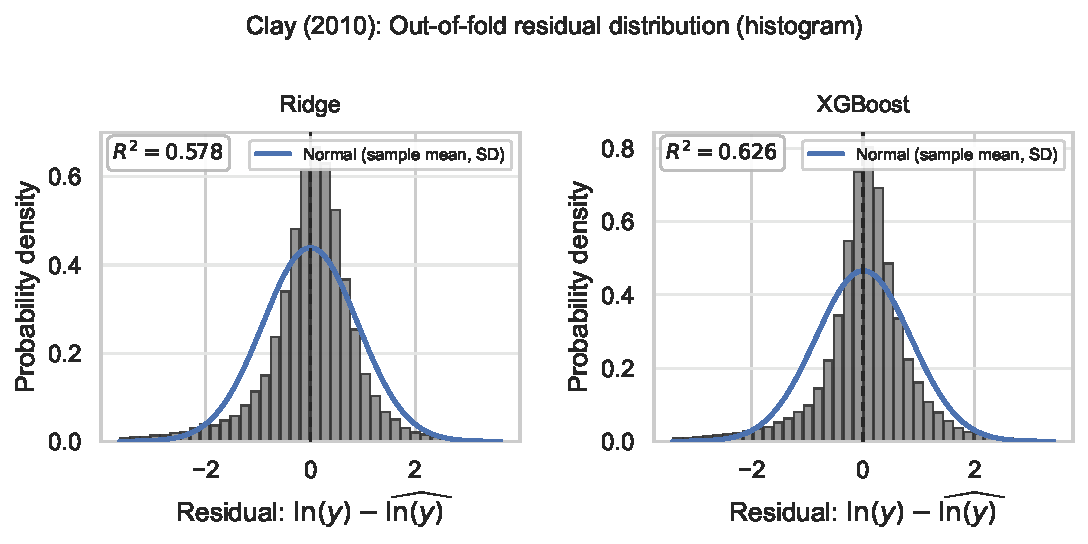
\includegraphics[width=\linewidth]{figs/oof_residuals_clay2010.pdf}
    \caption{Clay (2010 labels)}
    \label{fig:oof_clay2010}
  \end{subfigure}

  \caption{OOF calibration (top of each panel: predicted vs.\ realized $\ln(y)$ hexbins (indicating cell counts on a $\log_{10}$ scale) with identity line) and residual distributions (bottom of each panel: histogram with Gaussian overlay). (a) and (b) share 2020 labels; (c) uses 2010 labels.}
  \label{fig:oof_calibration_all}
\end{figure}

\subsection{Spatial Heterogeneity at State Scale}
\label{subsec:state_heterogeneity}

Another flaw of only looking at performance data aggregated to the national level is that it can conceal geography-dependent difficulties---which are precisely the settings motivating localized shocks such as mining corridors or tournament-driven population pulses discussed in Section \ref{sub:contextandmotivation}. This section attempts to address this by summarizing state-level performance. 

Figure \ref{fig:spatial_state_r2} summarizes the ridge and XGBoost polygon out-of-fold performance by Mexican state. Across all three embedding setups, large, northern states in Mexico seem to perform the best, whereas smaller, southern coastal states perform the worst. Clay (2010) appears to be the biggest outlier to this trend, likely because its evaluation is restricted to matched urban AGEBs which have higher baseline densities and lower spatial variance than the full 2020 census grid.

See Appendix \ref{appendix:state_level_figures} for figures on the mean absolute error by state (Figure \ref{fig:spatial_state_mae}) and the full table of $R^2$ results by state (Table \ref{fig:statebystate_table}).


\begin{figure}[H]
  \centering
  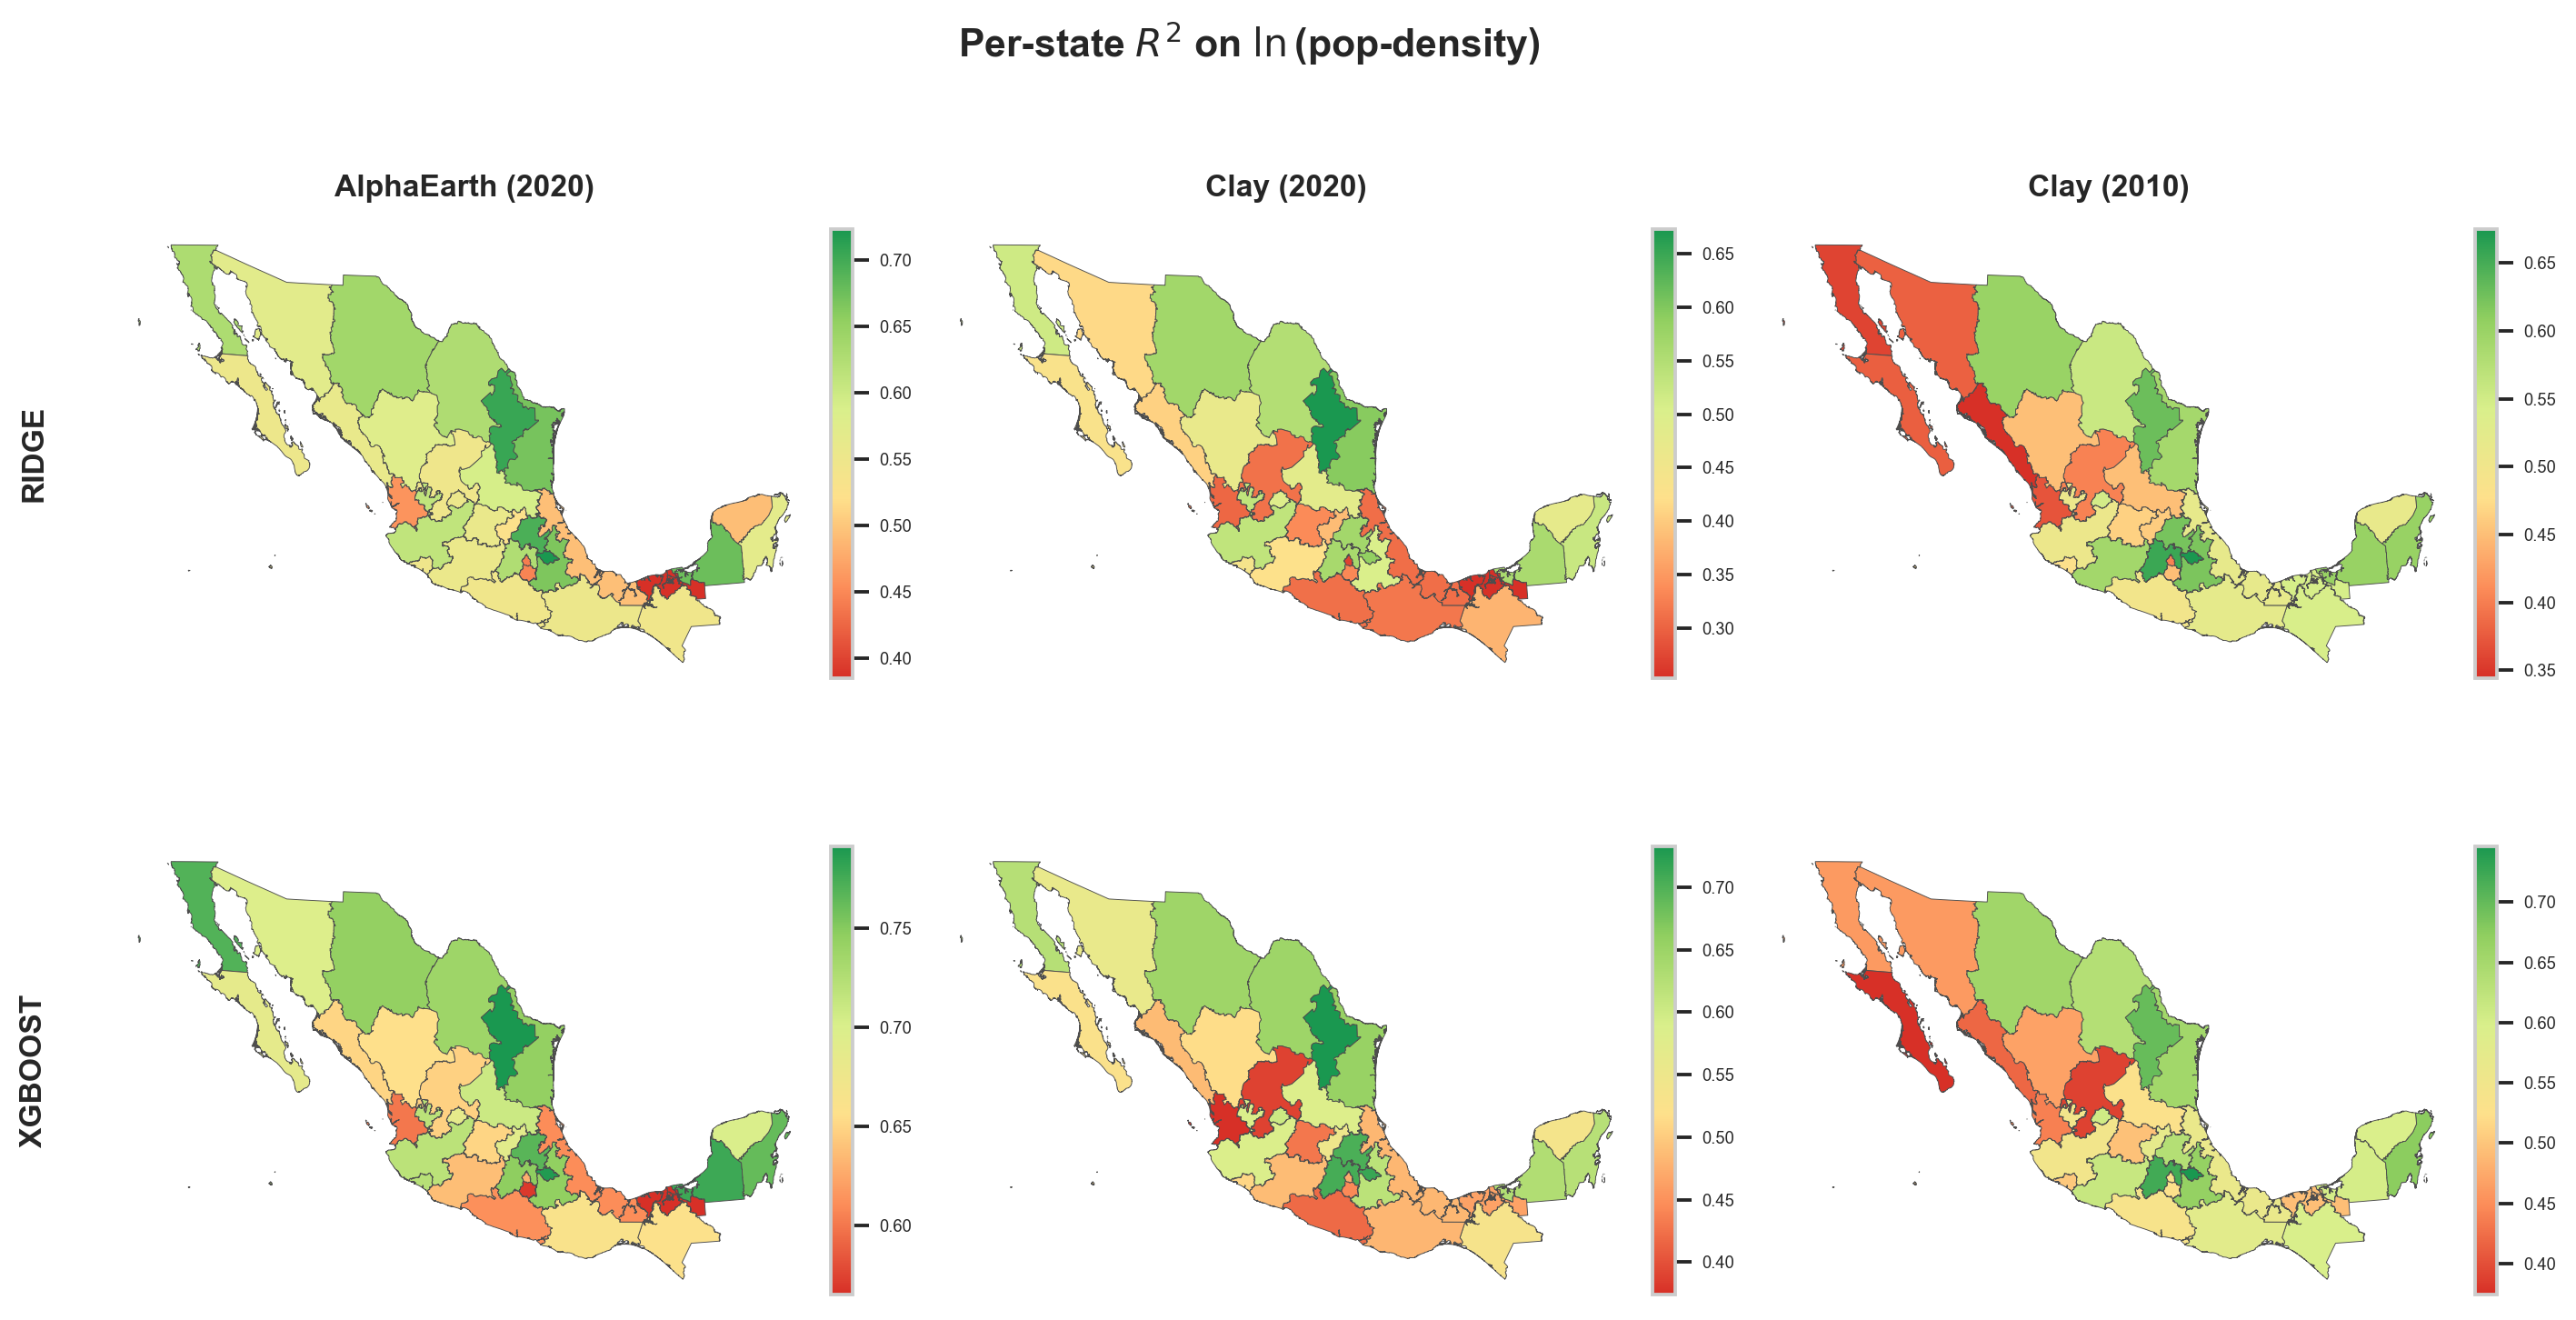
\includegraphics[width=\linewidth]{figs/spatial_state_r2.png}
  \caption{State choropleths of polygon-scale out-of-fold $R^2$ on $\ln(y)$ (left to right: AlphaEarth 2020, Clay 2020, Clay 2010). Top row: Ridge; bottom row: XGBoost. A shared green-to-red color scale is used across all panels for direct comparison. Color scale represents $R^2$: green indicates higher $R^2$; red indicates lower $R^2$.}
  \label{fig:spatial_state_r2}
\end{figure}


% ---- Drivers of state-level performance differences ----
\subsubsection{Drivers of State-Level Performance Differences}
\label{subsec:drivers_state}

The above sections have revealed that prediction quality varies across states. This section aims to figure out what drives this variation. For each embedding setup and model head combination (6 in total), I calculated each state's out-of-fold $R^2$ against several observable data characteristics: sample size ($n$), within-state target variance ($\mathrm{Var}[\ln y]$), mean polygon area, median polygon area, and urban AGEB fraction ($f_{\mathrm{urb}}$). The averaged results across all embedding setup and model head combination are shown in Table \ref{tab:avgcharacteristics}. Full table results and scatterplots are available in Appendix \ref{appendix:drivers} as Table \ref{tab:full_table_data_characteristics_importance} and Figures \ref{fig:state_r2_drivers_alphaearth_2020_ridge}-\ref{fig:state_r2_drivers_clay_2020_xgboost} respectively.

\begin{table}[H]
  \centering
  \caption{Aggregated summary of dataset characteristics. Columns provide the average Pearson correlation coefficient ($r$), the standard deviation of $r$ across tests, the count of tests achieving statistical significance ($p < 0.05$), and the overall significance rate across the 6 combinations of embedding sets and model head.}
  \label{tab:avgcharacteristics}
  \footnotesize
  \renewcommand{\arraystretch}{1.15}
  \setlength{\tabcolsep}{8pt}
  \begin{tabular}{@{} l cccc @{}}
    \toprule
    \textbf{Characteristic} & \textbf{Avg Pearson r} & \textbf{r Std Dev} & \textbf{Times Significant} & \textbf{Significance Rate (\%)} \\ 
    \midrule
    Median Area (km$^2$) & \cellcolor{teal!15}{0.598} & 0.065 & 6 & 100.0\% \\
    Mean Area (km$^2$)   & \cellcolor{teal!15}{0.582} & 0.081 & 6 & 100.0\% \\
    Target Variance      & 0.368 & 0.217 & 4 & 66.7\% \\
    Fraction Urban       & 0.222 & 0.100 & 0 & 0.0\% \\
    Sample Size ($N$)    & 0.023 & 0.150 & 0 & 0.0\% \\
    \bottomrule
  \end{tabular}

  \medskip
  \raggedright
  \textit{Notes:} \colorbox{teal!15}{Highlighted} cells indicate the top-performing characteristics by average Pearson correlation. Significance is determined at the $\alpha = 0.05$ level.
\end{table}

The strongest predictors of state-level performance are median and mean polygon areas, with average Pearson correlations ($r$) of $+0.598$ and $+0.582$ respectively. Larger polygons contain more satellite pixels, which means that the area-weighted or centroid-sampled embedding aggregated to the polygon has been averaged over a richer spatial context, dampening single-pixel noise. This suggests that the ratio between the spatial support of the remote sensing data and the size of the unit of analysis is an important determinant of model performance. 

Within-state target variance of $\ln(\text{population density})$ also played a strong predictive role with a Pearson correlation of $r=+0.368$. Intuitively, states whose polygons exhibit a wider spread of log densities---mixing rural and urban contexts---give the model more signal to separate. 

In contrast, the number of polygons per state is essentially uncorrelated with $R^2$ ($r = +0.023$), indicating that the models are not simply overfitting to larger states.

\paragraph{Other Explanations.} Another more qualitative---and more speculative---driver of the performance across states is landscape biome. \emph{Tabasco} consistently ranks as the worst-predicted state. Its landscape is dominated by low-lying wetlands, mangroves, and petroleum infrastructure, which may produce satellite signatures that the geospatial foundation models associates ambiguously with both uninhabited wetland and peri-urban settlement. This could compress the embedding space in a way that confuses the downstream prediction heads.  



\subsubsection{Systematic Prediction Bias by State}
\label{subsec:bias_choropleths}

Another interesting question is whether there is a systematic bias to the prediction errors by state. In other words, does the model systematically over- or under-predict population density in certain regions? Figure~\ref{fig:spatial_state_bias} maps the mean residual $\bar{e}_s = \frac{1}{n_s}\sum_{p \in s}(\widehat{\ln y_p} - \ln y_p)$ for each state $s$, separately for ridge (top row) and XGBoost (bottom row) across all three embedding setups. Red shading indicates states where the model, on average, predicts higher log-density than observed (over-prediction); blue indicates under-prediction.

\begin{figure}[H]
  \centering
  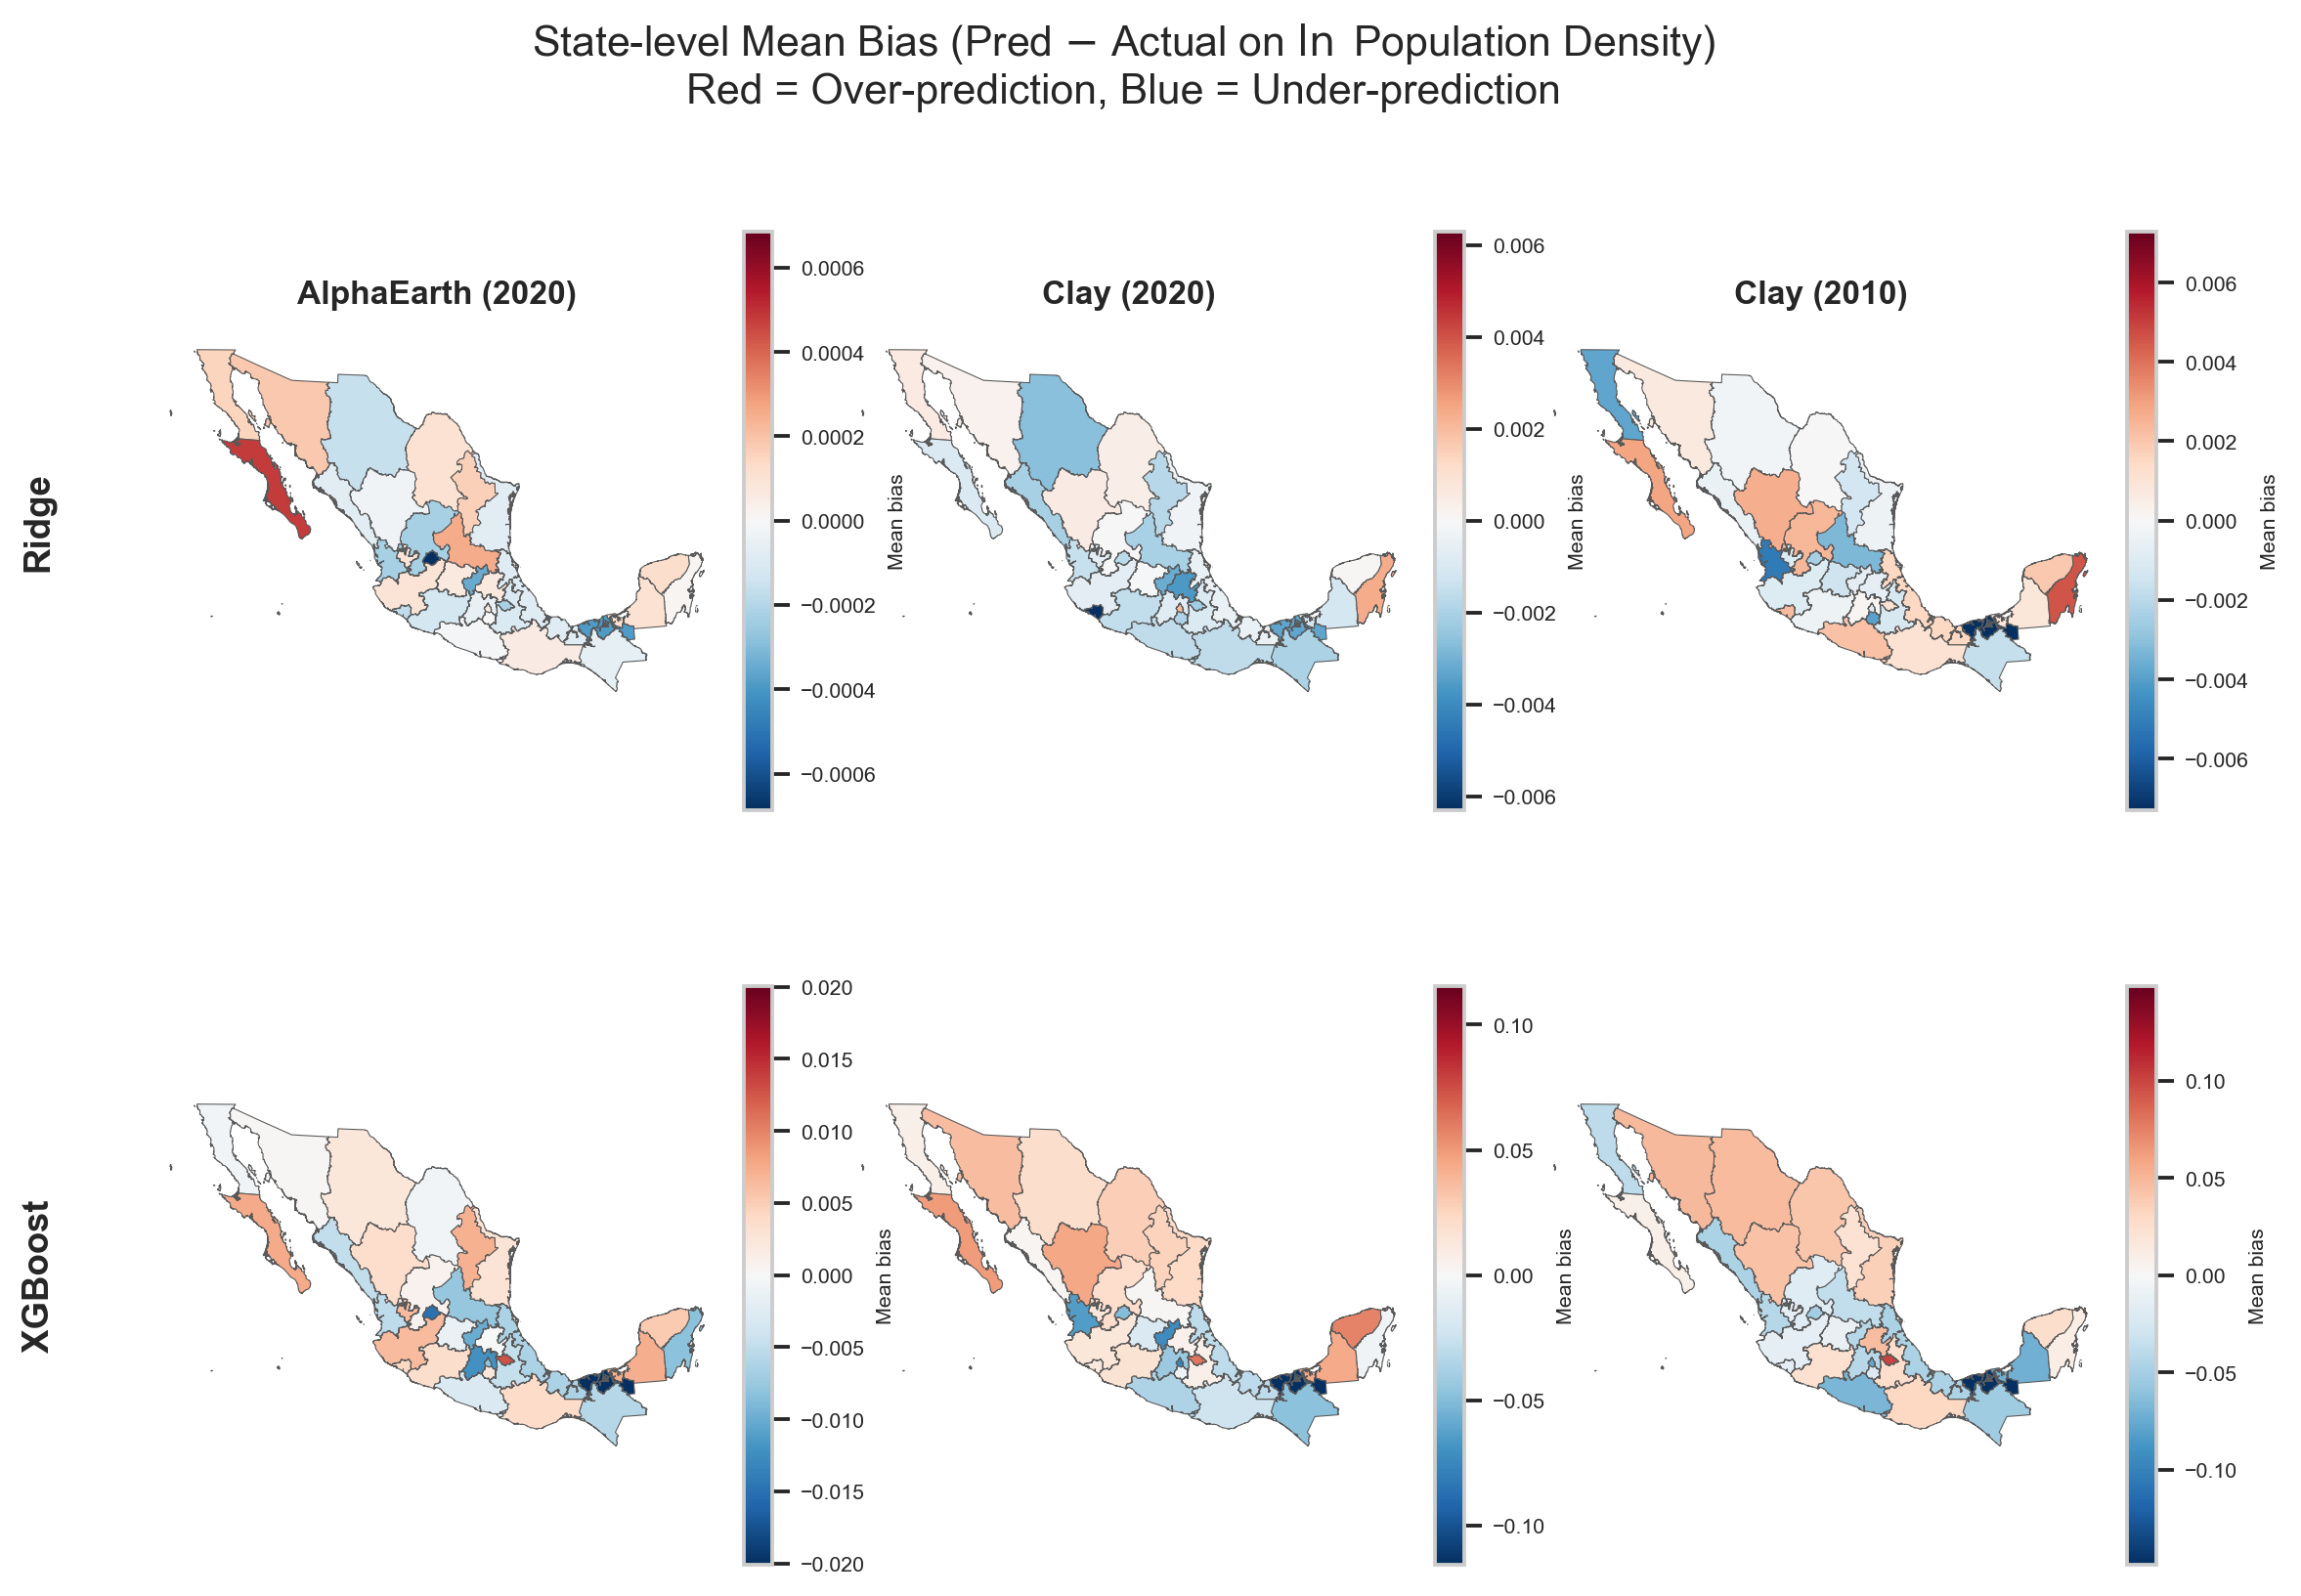
\includegraphics[width=\linewidth]{figs/spatial_state_bias.png}
  \caption{State-level mean bias (predicted $-$ actual $\ln$-density) across embedding sources and prediction heads. \textbf{Rows:} Ridge (top) and XGBoost (bottom). \textbf{Columns:} AlphaEarth (2020), Clay (2020), Clay (2010). Red = systematic over-prediction; blue = under-prediction. Note that AlphaEarth's color scale ($\pm 0.001$) is orders of magnitude narrower than Clay's ($\pm 0.3$), reflecting its superior calibration.}
  \label{fig:spatial_state_bias}
\end{figure}

One key observation from this figure is that AlphaEarth is nearly unbiased compared to Clay. Its mean bias ranges from roughly $-0.0007$ to $+0.0007$ for Ridge and $-0.02$ to $+0.01$ for XGBoost. This near-zero systematic bias across all 32 states is consistent with AlphaEarth's higher overall $R^2$ and suggests that the 10\,m embedding captures enough local variation to avoid persistent geographic lean in either direction.

Clay, on the other hand, exhibits substantially larger bias magnitudes (up to $\pm 0.36$ log units under Ridge). Northern industrialized states (e.g., Chihuahua, Nuevo León, and Tlaxcala) are consistently over-predicted, suggesting that the Clay embedding may associate their land-cover signatures (arid terrain, industrial clusters) with higher densities than actually observed. Conversely, southern and coastal states (e.g., Tabasco, Guerrero, Nayarit, and Mexico City) tend to be under-predicted. These directional patterns are broadly stable across both Ridge and XGBoost models, indicating that the bias originates in the embedding representation rather than the prediction head.




% \paragraph{Clay shows geographic bias patterns.}
% Both Clay columns exhibit substantially larger bias magnitudes (up to $\pm 0.36$ log units under ridge). Several patterns emerge. Northern industrialized states---Chihuahua, Nuevo León, and Tlaxcala---are consistently over-predicted, suggesting that the Clay embedding may associate their land-cover signatures (arid terrain, industrial clusters) with higher densities than actually observed. Conversely, southern and coastal states---Tabasco, Guerrero, Nayarit, and Ciudad de México---tend to be under-predicted. Tabasco's under-prediction reinforces the earlier observation that its wetland-dominated landscape confuses the encoder. CDMX's under-prediction is notable: despite being the densest state, the model undershoots its density, likely because CDMX's extreme homogeneity pushes predictions toward a national average that falls below CDMX's actual mean. These directional patterns are broadly stable across both ridge and XGBoost, indicating that the bias originates in the embedding representation rather than the prediction head.



\subsection{Predicting Change over Time}

The second research question shifts emphasis from cross-sectional levels to cross-decadal predication using Clay embeddings aligned with both census years. All three temporal experiments predict the \emph{2020} $\ln$-density label, but do so with varying inputs:
\begin{enumerate}
  \item \emph{Static baseline (2010-only embeddings):} Predict 2020 outcomes using embeddings derived solely from 2010 imagery.
  
  \item \emph{Change-augmented features (embedding deltas):} Predict 2020 outcomes using both 2010 embeddings and temporal differences $\Delta = \mathrm{emb}_{2020} - \mathrm{emb}_{2010}$ on matched units.
  
  \item \emph{Full-sample temporal transfer (no hold-out):} Train on all labeled 2010 polygons and predict across the full 2020 set without fold-wise holdout.
\end{enumerate}


Table~\ref{tab:clay_temporal_cross_year} isolates those protocols for ridge and XGBoost. Rows one and two share the identical matched AGEB intersection ($n\approx 52\mathrm{k}$) and identical randomized five-fold OOF splits so differences isolate feature engineering rather than sample composition. Row three deliberately sacrifices comparable CV discipline for coverage ($n\approx 106\mathrm{k}$).

% \begin{table}[H]
%   \centering
%   \caption{Clay cross-decadal experiments: $\ln(\text{population density})$ prediction of the 2020 label.}
%   \label{tab:clay_temporal_cross_year}
%   \footnotesize
%   \renewcommand{\arraystretch}{1.15}
%   \setlength{\tabcolsep}{4pt}
  
%   \begin{tabularx}{\textwidth}{@{} >{\raggedright\arraybackslash}X cccc r @{}}
%     \toprule
%     \textbf{Specification} & Ridge $R^2$ & Ridge MAE & XGB $R^2$ & XGB MAE & $n$ \\
%     \midrule
%     1. 2010 emb $\to$ 2020 (matched AGEBs, 5-fold OOF) & 0.5533 & 0.5741 & 0.6084 & 0.5277 & 52{,}086 \\
%     \addlinespace[4pt]
%     2. $[\mathrm{emb}_{2010},\,\Delta\mathrm{emb}] \to$ 2020 (matched AGEBs, 5-fold OOF) & \cellcolor{teal!15} 0.6121 & \cellcolor{teal!15} 0.5299 & \cellcolor{teal!15} 0.6389 & \cellcolor{teal!15} 0.5036 & 52{,}086 \\
%     \addlinespace[4pt]
%     3. Train all 2010 $\to$ predict 2020 (full 2020 grid; no OOF) & 0.3668 & 0.7255 & 0.4555 & 0.6617 & 106{,}564 \\
%     \bottomrule
%   \end{tabularx}
%   \medskip
%   \raggedright
%   \textit{Notes:} Row 3 is not cross-validated on the 2020 fold structure used in rows 1--2, so $R^2$ and MAE metrics are not directly comparable beyond qualitative reading. \colorbox{teal!15}{Highlighted} cells indicate the specification with best performance (highest $R^2$ and lowest MAE).
% \end{table}

\begin{table}[H]
  \centering
  \caption{Clay cross-decadal experiments: $\ln(\text{population density})$ prediction of the 2020 label.}
  \label{tab:clay_temporal_cross_year}
  \footnotesize
  \renewcommand{\arraystretch}{1.15}
  \setlength{\tabcolsep}{4pt}
  
  \begin{tabularx}{\textwidth}{@{} >{\raggedright\arraybackslash}X cccc r @{}}
    \toprule
    \textbf{Specification} & \textbf{Ridge $R^2$} & \textbf{Ridge MAE} & \textbf{XGB $R^2$} & \textbf{XGB MAE} & \textbf{$n$} \\
    \midrule
    1. 2010 emb $\to$ 2020 (matched AGEBs, 5-fold OOF) & 0.5533 & 0.5741 & 0.6084 & 0.5277 & 52,086 \\
    \addlinespace[4pt]
    2. $[\mathrm{emb}_{2010},\,\Delta\mathrm{emb}] \to$ 2020 (matched AGEBs, 5-fold OOF) & \cellcolor{teal!15}{0.6121} & \cellcolor{teal!15}{0.5299} & \cellcolor{teal!15}{0.6389} & \cellcolor{teal!15}{0.5036} & 52,086 \\
    \addlinespace[4pt]
    3. Train all 2010 $\to$ predict 2020 (full 2020 grid; no OOF) & 0.3668 & 0.7255 & 0.4555 & 0.6617 & 106,564 \\
    \bottomrule
  \end{tabularx}
  \medskip
  \raggedright
  \textit{Notes:} Row 3 is not cross-validated on the 2020 fold structure used in rows 1--2, so $R^2$ and MAE metrics are not directly comparable beyond qualitative reading. \colorbox{teal!15}{Highlighted} cells indicate the specification with best performance (highest $R^2$ and lowest MAE).
\end{table}

The results indicate that stacking $\Delta\mathrm{emb}$ modestly but uniformly improves both heads relative to the 2010-embedding baseline on the matched panel. This suggests that measurable satellite-side drift between surveys carries usable signal beyond static encodings. It also corroborates what \textcite{Burns2026} found about the benefits of preserving full embedding delta vs. collapsing the delta to a scalar magnitude. Unsurprisingly, the transfer specification (3) performed the worst despite doubling effective evaluation units. This is consistent with covariate shift once predictions extrapolate from the historical training universe to the full modern polygon canvas.

\subsubsection{Temporal Case Studies}
\label{sub:temporal_case_studies}

To assess whether the aggregate temporal correlations manifest as spatially coherent patterns at the city level, Figure~\ref{fig:case_study_temporal} maps actual versus predicted $\Delta\ln(\text{population density})$ for three municipalities with high Pearson $r$ scores: \emph{Querétaro} ($r = 0.567$, $n = 312$), \emph{Cancún} ($r = 0.633$, $n = 314$), and \emph{Aguascalientes} ($r = 0.678$, $n = 279$). Predictions use the best temporal specification (Clay, $[\mathrm{emb}_{2010},\,\Delta\mathrm{emb}] \to$ 2020, XGBoost).

\begin{figure}[htbp]
  \centering
  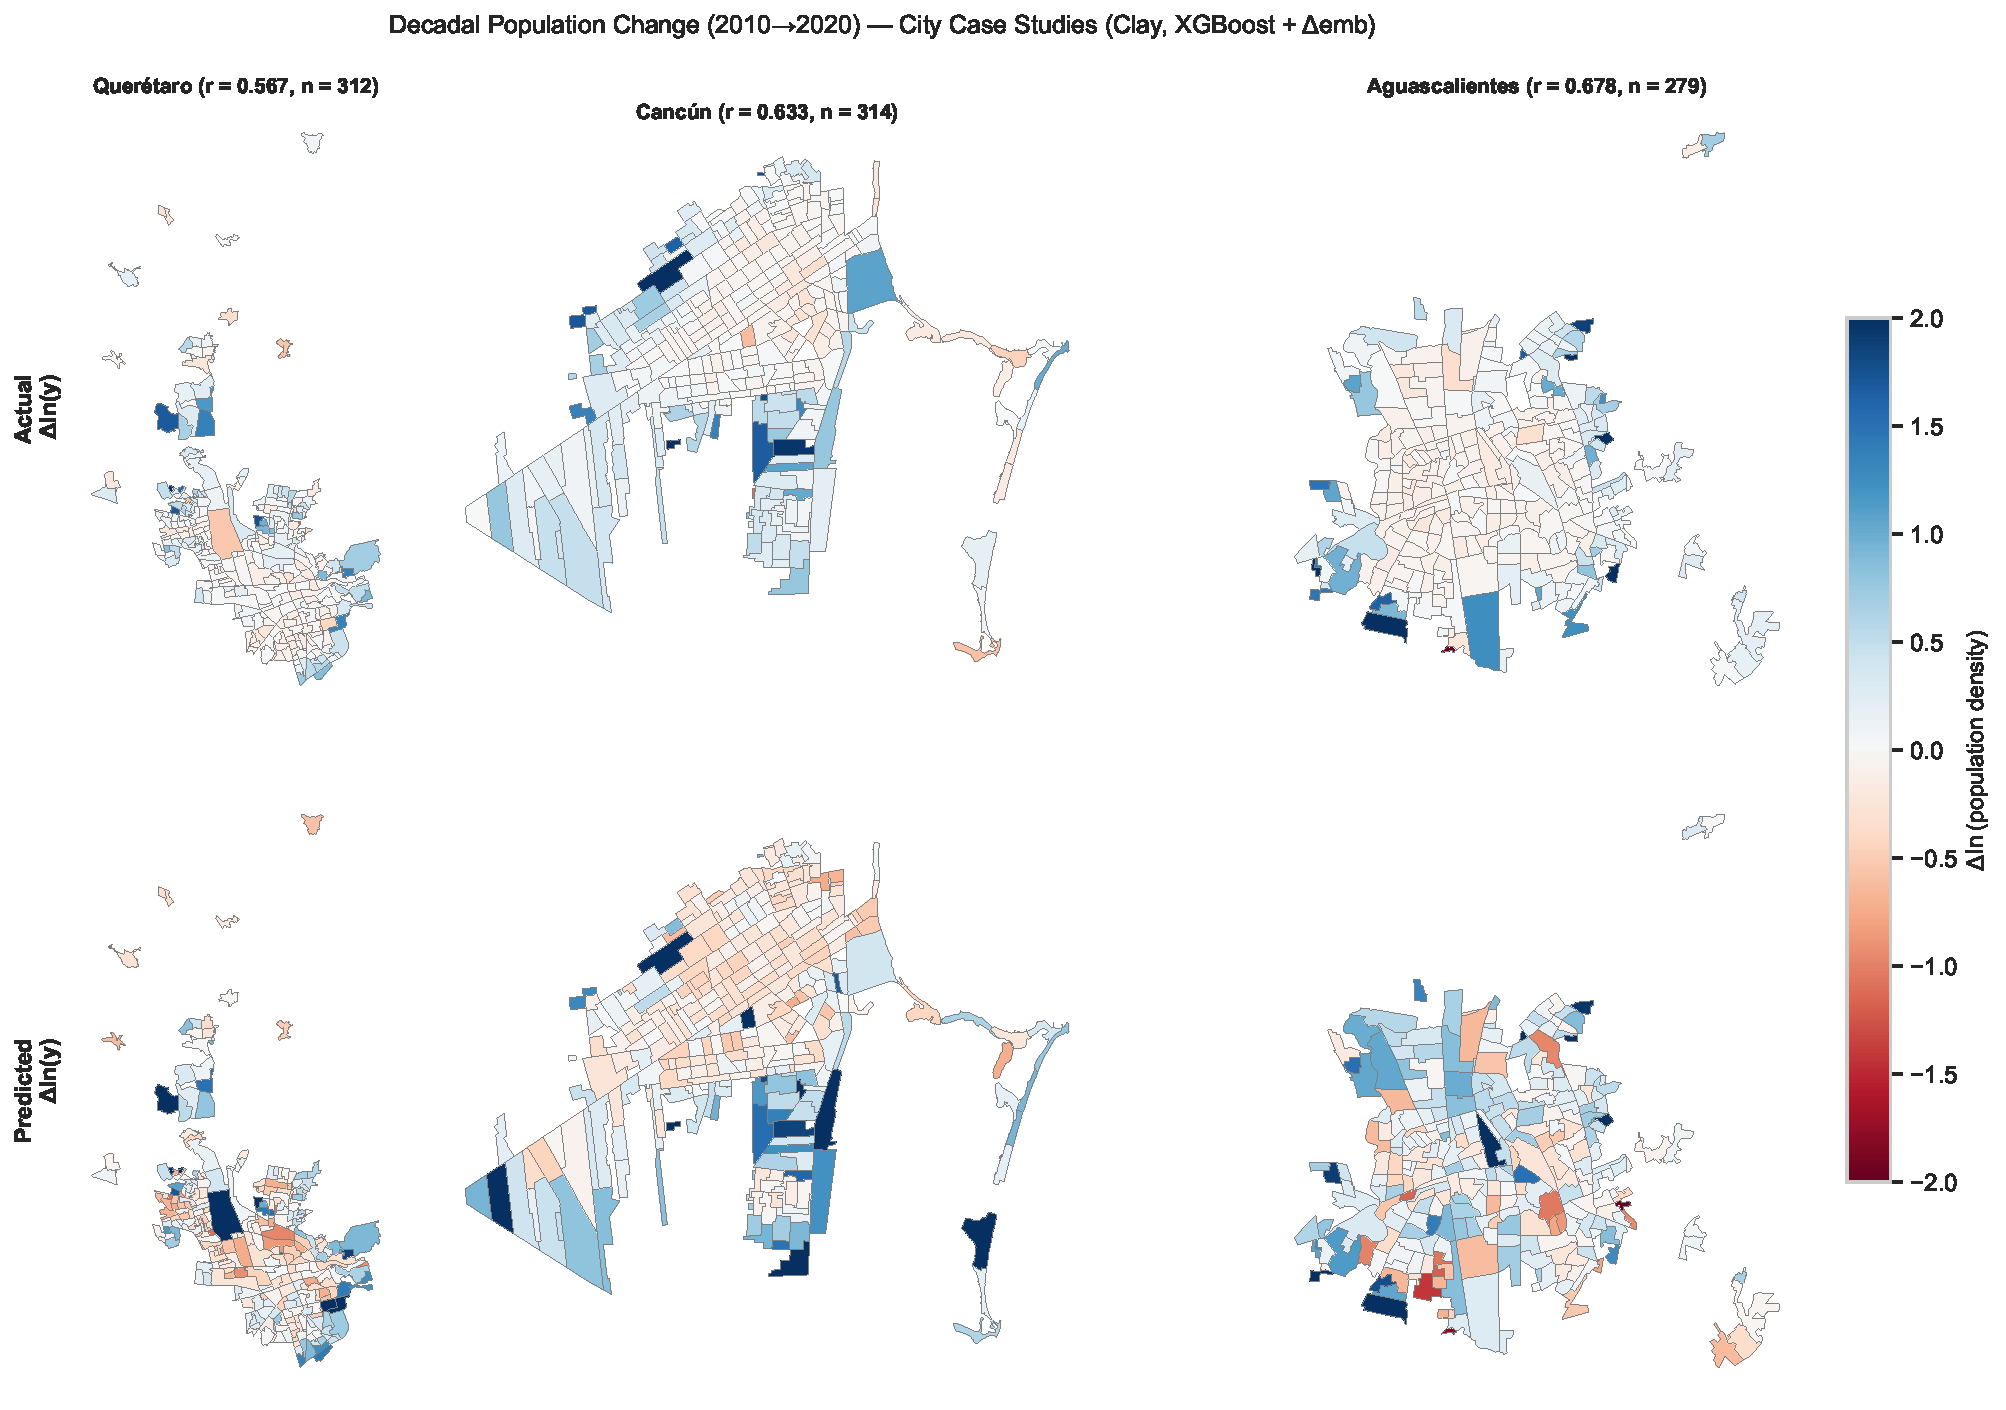
\includegraphics[width=\textwidth]{figs/case_study_temporal_change.pdf}
  \caption{Actual (top) versus predicted (bottom) decadal change $\Delta\ln(\text{pop.\ density})$ for the municipalities of Querétaro, Cancún, and Aguascalientes. Blue indicates population growth, red indicates decline. Color scale is shared within each city column using a diverging red-to-blue palette centered at zero.}
  \label{fig:case_study_temporal}
\end{figure}

All three cities exhibit a common suburbanization signature---peripheral AGEBs colored in blue (growth) ringing an older core with near-zero or mildly negative change---and the predicted maps reproduce this spatial gradient with reasonable fidelity. In Cancún, the model correctly identifies rapid densification along the northern hotel-zone corridor and westward residential expansion, while the established downtown grid registers as near-zero change in both actual and predicted panels. Aguascalientes, a compact radial city, yields the highest municipality-level $r$ likely because the model captures both the outer growth ring and scattered interior pockets of densification. Querétaro, despite a lower $r$ at the municipality level than at the state level ($0.567$ vs.\ $0.669$), still shows spatial agreement in the broad pattern---growth in the southern satellite towns and relative stagnation in the historic center---though the prediction underestimates the magnitude of peripheral growth in several fast-developing AGEBs.

These maps demonstrate that the temporal signal encoded in $\Delta\mathrm{emb}$ is not merely statistical noise driving aggregate correlations; it translates into spatially interpretable growth patterns that align with known urbanization dynamics in Mexican secondary cities.

\subsubsection{Calibration and Residual Diagnostics}

Next, I investigated whether modeled $\ln(y_{2020})$ implies coherent decadal change relative to realized $\ln(y_{2010})$ on matched polygons (this is a similar approach to Section \ref{sub:calibration_diagnostics}). Define $\Delta\ln(y)=\ln(y_{2020})-\ln(y_{2010})$ and analogously predicted change $\widehat{\Delta}=\widehat{\ln(y_{2020})}-\ln(y_{2010})$ using each prediction column from the three Clay setups. Figure~\ref{fig:temporal_change_cross_temporal} plots $\widehat{\Delta}$ vs. $\Delta\ln(y)$ using hexbins (darker cells accumulate mass where many AGEBs co-locate in $(\Delta_{\mathrm{act}},\Delta_{\mathrm{pred}})$ space). 

Because decadal adjustments on the log scale are often modest relative to cross-sectional dispersion across Mexico, absolute squared-error scores on $\Delta$ alone can be harsh even when predictions preserve directional ranking across settlements. Thus, I recorded the Pearson $r$ in addition to the $R^2$ to get a better sense of whether the model was able to preserve the directional ranking of decadal change (i.e., whether growing polygons tend to receive larger predicted increments than shrinking ones).

\begin{figure}[H]
  \centering
  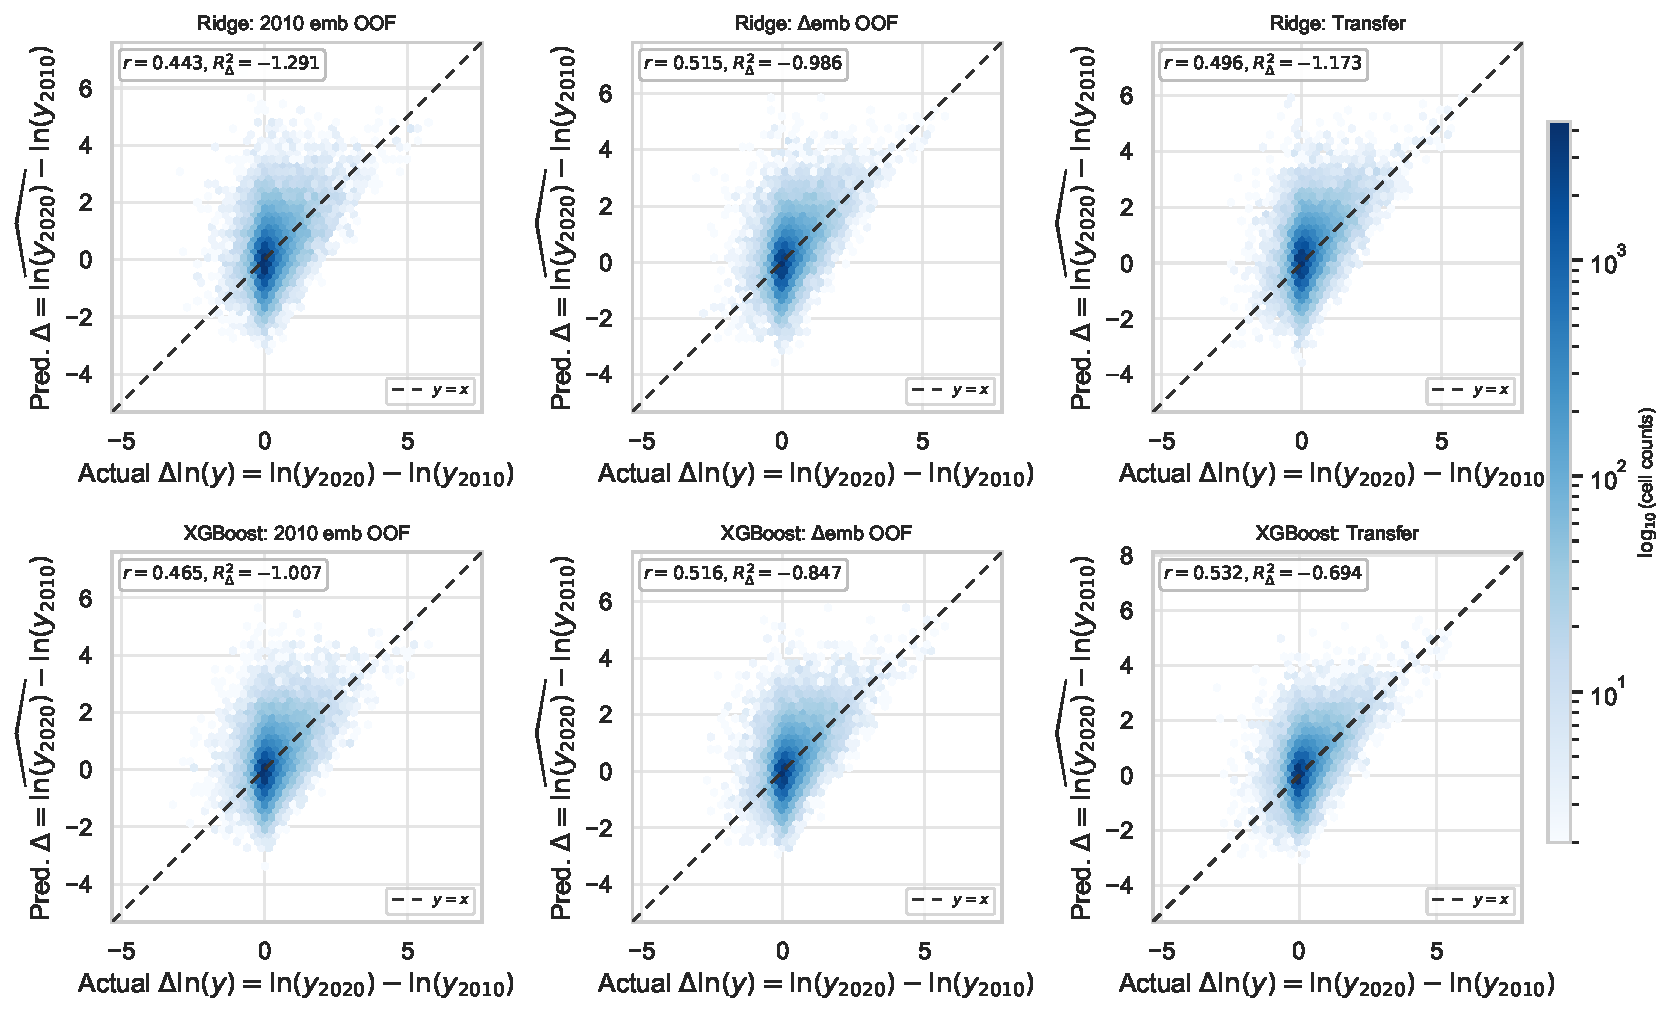
\includegraphics[width=\linewidth]{figs/temporal_change_hexbin_cross_temporal.pdf}
  \caption{Clay, matched 2010--2020 AGEBs: hexbin plots of actual versus predicted $\Delta\ln(y)$ under three cross-decadal prediction setups (columns). Rows: Ridge and XGBoost. Axis annotations report Pearson $r$ and $R^2$ on $\Delta$ per panel.}
  \label{fig:temporal_change_cross_temporal}
\end{figure} 

All models achieve a moderate positive correlation, ranging from $0.443$ to $0.532$. This suggests the models are successfully capturing the directional ranking of change. However, the universally negative $R^2$ values suggest that decadal population shifts are modest relative to the residual noise in satellite-derived embeddings, meaning the model follows the general trend without accurately scaling the magnitude of change. Thus, these results suggest that even though these models' satellite-derived embeddings cannot predict exact population changes over time, they do carry statistically significant signal for identifying the direction of growth across the Mexican landscape.

\newpage

\section{Conclusion}
\subsection{Discussion of Results}
The findings of this thesis suggest that geospatial foundation models can do a decent job at bridging the gap between decennial censuses and the immediate needs of policymakers. While a traditional national count, requires the mobilization of hundreds of thousands of workers (Mexico's 2020 Censo de Población y Vivienda had $151,000$ interviewers \parencite{inegi2020censo}) and a budget of billions of dollars (the 2020 US Census cost $13.7$ billion and reports indicate the cost of the census has doubled in the past decade \parencite{gao2023census, farmer2018census}), the models explored in this thesis can produce high-resolution population estimates using only a few hours of compute resources. Empirically, these models explain between $61\%$ and $73\%$ of the variation in log population density at the polygon level. Perhaps more significantly for regional planning, predictive accuracy scales with geographic aggregation, achieving an $R^2$ of up to $0.88$ at the municipality level (AlphaEarth, 2020, XGBoost). This demonstrates that while point-level noise persists in satellite-derived embeddings, the models capture the broad population dynamics of a region with impressive fidelity.

Comparing these results to the existing literature, my findings demonstrate that geospatial foundation models significantly push the boundary of what is possible in intercensal population estimation. At the polygon level, the AlphaEarth 2020 XGBoost $R^2$ of $0.727$ exceeds the $R^2 = 0.71$ achieved by task-specific urban CNNs at a similar 30\,m resolution in Nanjing \parencite{SONG2019103580}---a notable result given that my dataset spans the full geographic and morphological diversity of Mexico rather than a single metropolitan area. It also exceeds the $R^2$ of 0.63--0.64 that \textcite{metz2025application} found for Malawi population density prediction. Furthermore, my municipality-level $R^2$ of $0.879$ is very close to the $R^2 = 0.91$ benchmark cited for national-scale models operating at much coarser 250\,m resolutions \parencite{rs11222620}. 


\paragraph{Scale Effects on Model Performance.}
Statistical analysis of state-level performance reveals that median polygon area is the strongest predictor of model accuracy ($r=0.56$). This suggests that the vision transformer architecture benefits significantly from a richer window of pixels. Larger polygons, like those typical of Northern Mexican states, provide the model with more spatial context to resolve complex land-use patterns. Conversely, highly dense and structurally homogenous areas like Mexico City lack the within-state variance to enable embeddings to learn the subtle signals in density differences. The key takeaway is that model utility is highest when applied to units of analysis that align with the spatial support of the underlying remote sensing data.

\paragraph{Environmental Bias.}
For the Clay models, I found non-trivial amounts of systematic over/under-prediction that varied with the country's environmental features. There was persistent over-prediction in northern industrial states and a systematic under-prediction in southern, wetland-heavy regions such as Tabasco. This regional tilt suggests that the Clay embeddings may conflate specific land-cover signatures (e.g., arid terrain or industrial clusters) with higher population densities than are actually present. In the South, where dense vegetation and wetlands may mask informal settlements or specific roofing materials, the models tend to underestimate residents. Policymakers should note that these models, while computationally efficient, risk under-representing vulnerable populations in specific environmental contexts unless calibrated for local biomes.

\paragraph{Utility vs. Precision in Temporal Change Prediction.}
Predicting change over the decade between census years ($\Delta \ln y$) proved to be a significantly more challenging task than cross-sectional levels, as evidenced by universally negative $R^2$ values.  This is likely because decadal population adjustments are modest relative to the residual noise inherent in satellite embeddings. However, the moderate Pearson correlations ($r \approx 0.5$) achieved in these experiments indicate that the models effectively preserve the directional ranking of growth. From a policy perspective a model need not predict exact resident counts to be valuable. Even if it just correctly identifies the fastest-growing AGEBs, policymakers can use it to prioritize the placement of critical educational, medical, and electrical infrastructure between census cycles.

\paragraph{Synthesis.}
Echoing back to our initial research questions from Section \ref{sub:researchque}, the results successfully answer our first question and partially address the second. On question 1, both AlphaEarth and Clay predict population density at levels exceeding benchmarks in comparable intercensal literature, particularly when aggregated to the municipal scale. On question 2, while absolute change prediction remains high-variance, both models produce a statistically significant directional signal for identifying which areas are growing. Together, these findings position geospatial foundation models as high-frequency, cost-effective nowcasting tools that can prevent data staleness in rapidly developing nations. Their value is highest as heuristic instruments, providing insights into where to direct scarce enumeration resources, flagging where data staleness is most acute, and providing the directional signal about growth patterns that infrastructure planners need between census cycles. This is perhaps less exciting of a claim than replacing the decennial census, but it is also a more achievable and arguably more valuable one.


\subsection{Limitations}
\label{sub:limitation}

There are a few factors, ranging from data limitations to technical data processing specifications, that are limiting the potential of this project.

\paragraph{Absence of 2010 locality-level shapefiles.}
The 2010 INEGI census data did not include locality-level shapefiles comparable to those available for 2020, restricting the 2010 analysis to urban AGEBs exclusively. This introduced two compounding constraints: (1) the urban-only sample is definitionally homogeneous in settlement type, and (2) the reduced number of observations limited the model's training data. It also complicated direct comparison between 2010 and 2020 results, as performance differences cannot be cleanly attributed to model behavior versus differences in geographic scope and sample composition.

\paragraph{Zero-population filtering.}
To improve regression performance, AGEBs with zero recorded population were excluded from the analysis. While this affected only approximately $3\%$ of the dataset, it represents an abdication of a meaningful classification task. A more robust approach would distinguish between genuinely uninhabited land (e.g., industrial parks, conservation areas, and similar zones) and sparsely populated areas that may still warrant infrastructure planning. Future work should incorporate land-use classifications to handle this distinction explicitly rather than excluding these observations outright.

\paragraph{Potential measurement error in 2020 census labels.}
The 2020 Mexican Census was selected as the primary ground truth on the basis of recency and the availability of high-resolution satellite imagery for that period. However, 2020 was a tumultuous year for the world, primarily because of the COVID-19 pandemic. The census, conducted in March 2020, coincided with the worst of the pandemic. Disruptions to field operations and household response rates during this period may have introduced non-random measurement error into the ground truth labels. To the extent that the model is penalized for predicting high-density clusters in areas where the census systematically undercounted residents due to pandemic-related logistical failures, the reported $R^2$ values may understate the model's true predictive capability.


\subsection{Future Work}

The field of geospatial foundation models for predicting socioeconomic labels is still nascent. There are many areas to extend and build upon the findings of this thesis.

\paragraph{Two-Stage modeling for inhabited land classification.} As discussed in Section \ref{sub:limitation}, one flaw with the model is that it does not distinguish between genuinely uninhabited land and sparsely populated areas. Future work could extend my project with a two-stage model to first classify populated vs. unpopulated land, and then second perform the regression to predict exact population densities. 


\paragraph{Predict on additional target outcomes.} 
While this thesis focused strictly on population density, the ground-truth census data provided by INEGI contains a vast breadth of other critical socioeconomic indicators, like household wealth, that could serve as future prediction targets. Future research should investigate whether the latent embeddings produced by AlphaEarth and Clay can generalize to predict non-visual traits such as household wealth, educational attainment, or access to infrastructure. Because these foundation models are trained on massive, multimodal datasets, they may capture proxies for poverty, such as roof material, road quality, or agricultural patterns, that correlate with wealth indices. 

\paragraph{Apply to real-world localized population shocks.}
A promising application of high-frequency population density prediction is the monitoring of localized and temporary population shocks that traditional decennial censuses are structurally unable to capture. One timely example is the upcoming 2026 FIFA World Cup, which will be partially hosted in Mexico City, Guadalajara, and Monterrey, and will produce temporary but massive population concentrations. Using these foundation models to estimate the impact of these shocks on local labor markets and municipal services would provide planners with a dynamic measurement tool for infrastructure and resource allocation that traditional census data cannot offer.

\paragraph{Technical optimizations.}
Another area of future work could be to evaluate the Clay model using Landsat-8 imagery. While this study utilized Landsat-7 to maintain temporal consistency between 2010 and 2020, Landsat-8 offers superior signal-to-noise performance and an expanded spectral range. Investigating whether these sensor improvements allow the Clay model to match the high-resolution performance scores established by AlphaEarth's Sentinel-2 derived features would clarify whether performance gaps are driven by the foundation model architecture or the quality of the input data. Furthermore, future research should experiment with input chip sizes for the vision transformer architecture. This study utilized $128 \times 128$ pixel chips, but increasing the dimensions to $256 \times 256$ may provide a larger spatial receptive field, potentially improving the model's ability to resolve density in granular AGEB units where contextual land-use cues are critical. Finally, additional work could be done in integrating auxiliary data signals part of these foundation models, like mobile-phone metadata, social-connectivity proxies, and object-level features. These could help improve our population density predictions beyond just satellite imagery alone.


\paragraph{Practical engagement and policy communication.}
For any of this research to have tangible impact, there needs to be a robust framework for communicating these results to policymakers. Future work should focus on developing methods to convey model uncertainty and persistent biophysical biases, such as the under-prediction observed in wetland-heavy regions, to non-technical stakeholders. Without this transparency, algorithmic population estimates risk projecting a false sense of precision that could misdirect the very resource allocations they are intended to improve. If geospatial foundation models are to successfully transition from academic benchmarks to operational policy tools, communicating their blind spots must be treated with the same rigor as maximizing their predictive accuracy.

\newpage


\printbibliography[heading=bibintoc,title={References}]


\newpage


\appendix
\section{Hyperparameter Tuning Details}
\label{app:hyperparameters}

This appendix records the hyperparameter search spaces and strategies used for the ridge and XGBoost prediction heads (Section~\ref{sec:methodology} of the main text).

\begin{table}[H]
  \centering
  \caption{Clay 2010 and 2020 hyperparameter tuning search space and search strategies}
  \label{tab:hyperparameters}
  \setlength{\tabcolsep}{5pt}
  \renewcommand{\arraystretch}{1.15}
  \begin{tabularx}{\textwidth}{@{}
    >{\raggedright\arraybackslash}p{0.30\textwidth}
    X
    >{\raggedright\arraybackslash}p{0.16\textwidth}
  @{}}
  \toprule
  \textbf{Parameter} & \textbf{Search space / distribution} & \textbf{Strategy} \\
  \midrule
  \multicolumn{3}{@{}l}{\textbf{Ridge regression}} \\
  \addlinespace[2pt]
  $\alpha$ (regularization) &
  $\{10^{-3}, 10^{-2}, 10^{-1}, 1, 3, 10, 30,$ \newline
  $100, 300, 1000, 2500, 5000, 7500, 10000\}$ &
  Grid search \\
  \midrule
  \multicolumn{3}{@{}l}{\textbf{XGBoost (random search, 100 trials)}} \\
  \addlinespace[2pt]
  Learning rate ($\eta$) & $[0.01, 0.2]$ (log-uniform) & Random \\
  Max depth & $[3, 10]$ (integer) & Random \\
  Subsample & $[0.6, 1.0]$ (uniform) & Random \\
  \texttt{colsample\_bytree} & $[0.6, 1.0]$ (uniform) & Random \\
  \texttt{reg\_lambda} ($\lambda$) & $[10^{-3}, 100]$ (log-uniform) & Random \\
  \texttt{reg\_alpha} ($\alpha$) & $[10^{-3}, 10]$ (log-uniform) & Random \\
  \texttt{min\_child\_weight} & $[0.1, 50]$ (log-uniform) & Random \\
  Gamma ($\gamma$) & $[10^{-4}, 10]$ (log-uniform) & Random \\
  \midrule
  \multicolumn{3}{@{}l}{\textbf{Fixed parameters}} \\
  \addlinespace[2pt]
  \texttt{n\_estimators} & 2000 boosting rounds & Fixed \\
  Early stopping & 50 rounds & Fixed \\
  \midrule
  \textbf{Objective} & \textbf{Maximize $R^2$ under 5-fold CV} & \\
  \bottomrule
  \end{tabularx}
\end{table}

\begin{table}[H]
  \centering
  \caption{AlphaEarth (2020) hyperparameter tuning search space and search strategies}
  \label{tab:hyperparameters_alphaearth}
  \setlength{\tabcolsep}{5pt}
  \renewcommand{\arraystretch}{1.15}
  \begin{tabularx}{\textwidth}{@{}
    >{\raggedright\arraybackslash}p{0.30\textwidth}
    X
    >{\raggedright\arraybackslash}p{0.16\textwidth}
  @{}}
  \toprule
  \textbf{Parameter} & \textbf{Search space / distribution} & \textbf{Strategy} \\
  \midrule
  \multicolumn{3}{@{}l}{\textbf{Ridge regression (random search, 40 trials)}} \\
  \addlinespace[2pt]
  $\alpha$ (regularization) & $[10^{-3}, 10^{4}]$ (log-uniform) & Random \\
  \midrule
  \multicolumn{3}{@{}l}{\textbf{XGBoost (random search, 30 trials)}} \\
  \addlinespace[2pt]
  Learning rate ($\eta$) & $\{0.01, 0.05, 0.1, 0.2\}$ & Random \\
  Max depth & $\{4, 6, 8, 10\}$ & Random \\
  Subsample & $\{0.6, 0.7, 0.8, 0.9, 1.0\}$ & Random \\
  \texttt{colsample\_bytree} & $\{0.6, 0.7, 0.8, 0.9, 1.0\}$ & Random \\
  \texttt{reg\_lambda} ($\lambda$) & $\{0.5, 1.0, 2.0, 5.0\}$ & Random \\
  \texttt{reg\_alpha} ($\alpha$) & $\{0, 0.1, 0.5, 1.0\}$ & Random \\
  \texttt{min\_child\_weight} & $\{1, 3, 5, 7\}$ & Random \\
  Gamma ($\gamma$) & $\{0, 0.1, 0.2, 0.5\}$ & Random \\
  \texttt{n\_estimators} & $\{500, 800, 1000, 1200, 1500\}$ & Random \\
  \midrule
  \multicolumn{3}{@{}l}{\textbf{Fixed parameters}} \\
  \addlinespace[2pt]
  Ridge preprocessing & \texttt{StandardScaler} (fit on training folds) & Fixed \\
  \texttt{tree\_method} & \texttt{hist} & Fixed \\
  Training subset for tuning & 80\% of observations (train/test split, seed 42) & Fixed \\
  \midrule
  \textbf{Objective} & \textbf{Maximize $R^2$ under 3-fold CV} & \\
  \bottomrule
  \end{tabularx}
\end{table}

\newpage

\section{State-level Performance Figures}
\label{appendix:state_level_figures}

This appendix records the state-level error distributions and the complete state-by-state performance table (Section \ref{subsec:state_heterogeneity} of the main text).

\begin{figure}[htbp]
  \centering
  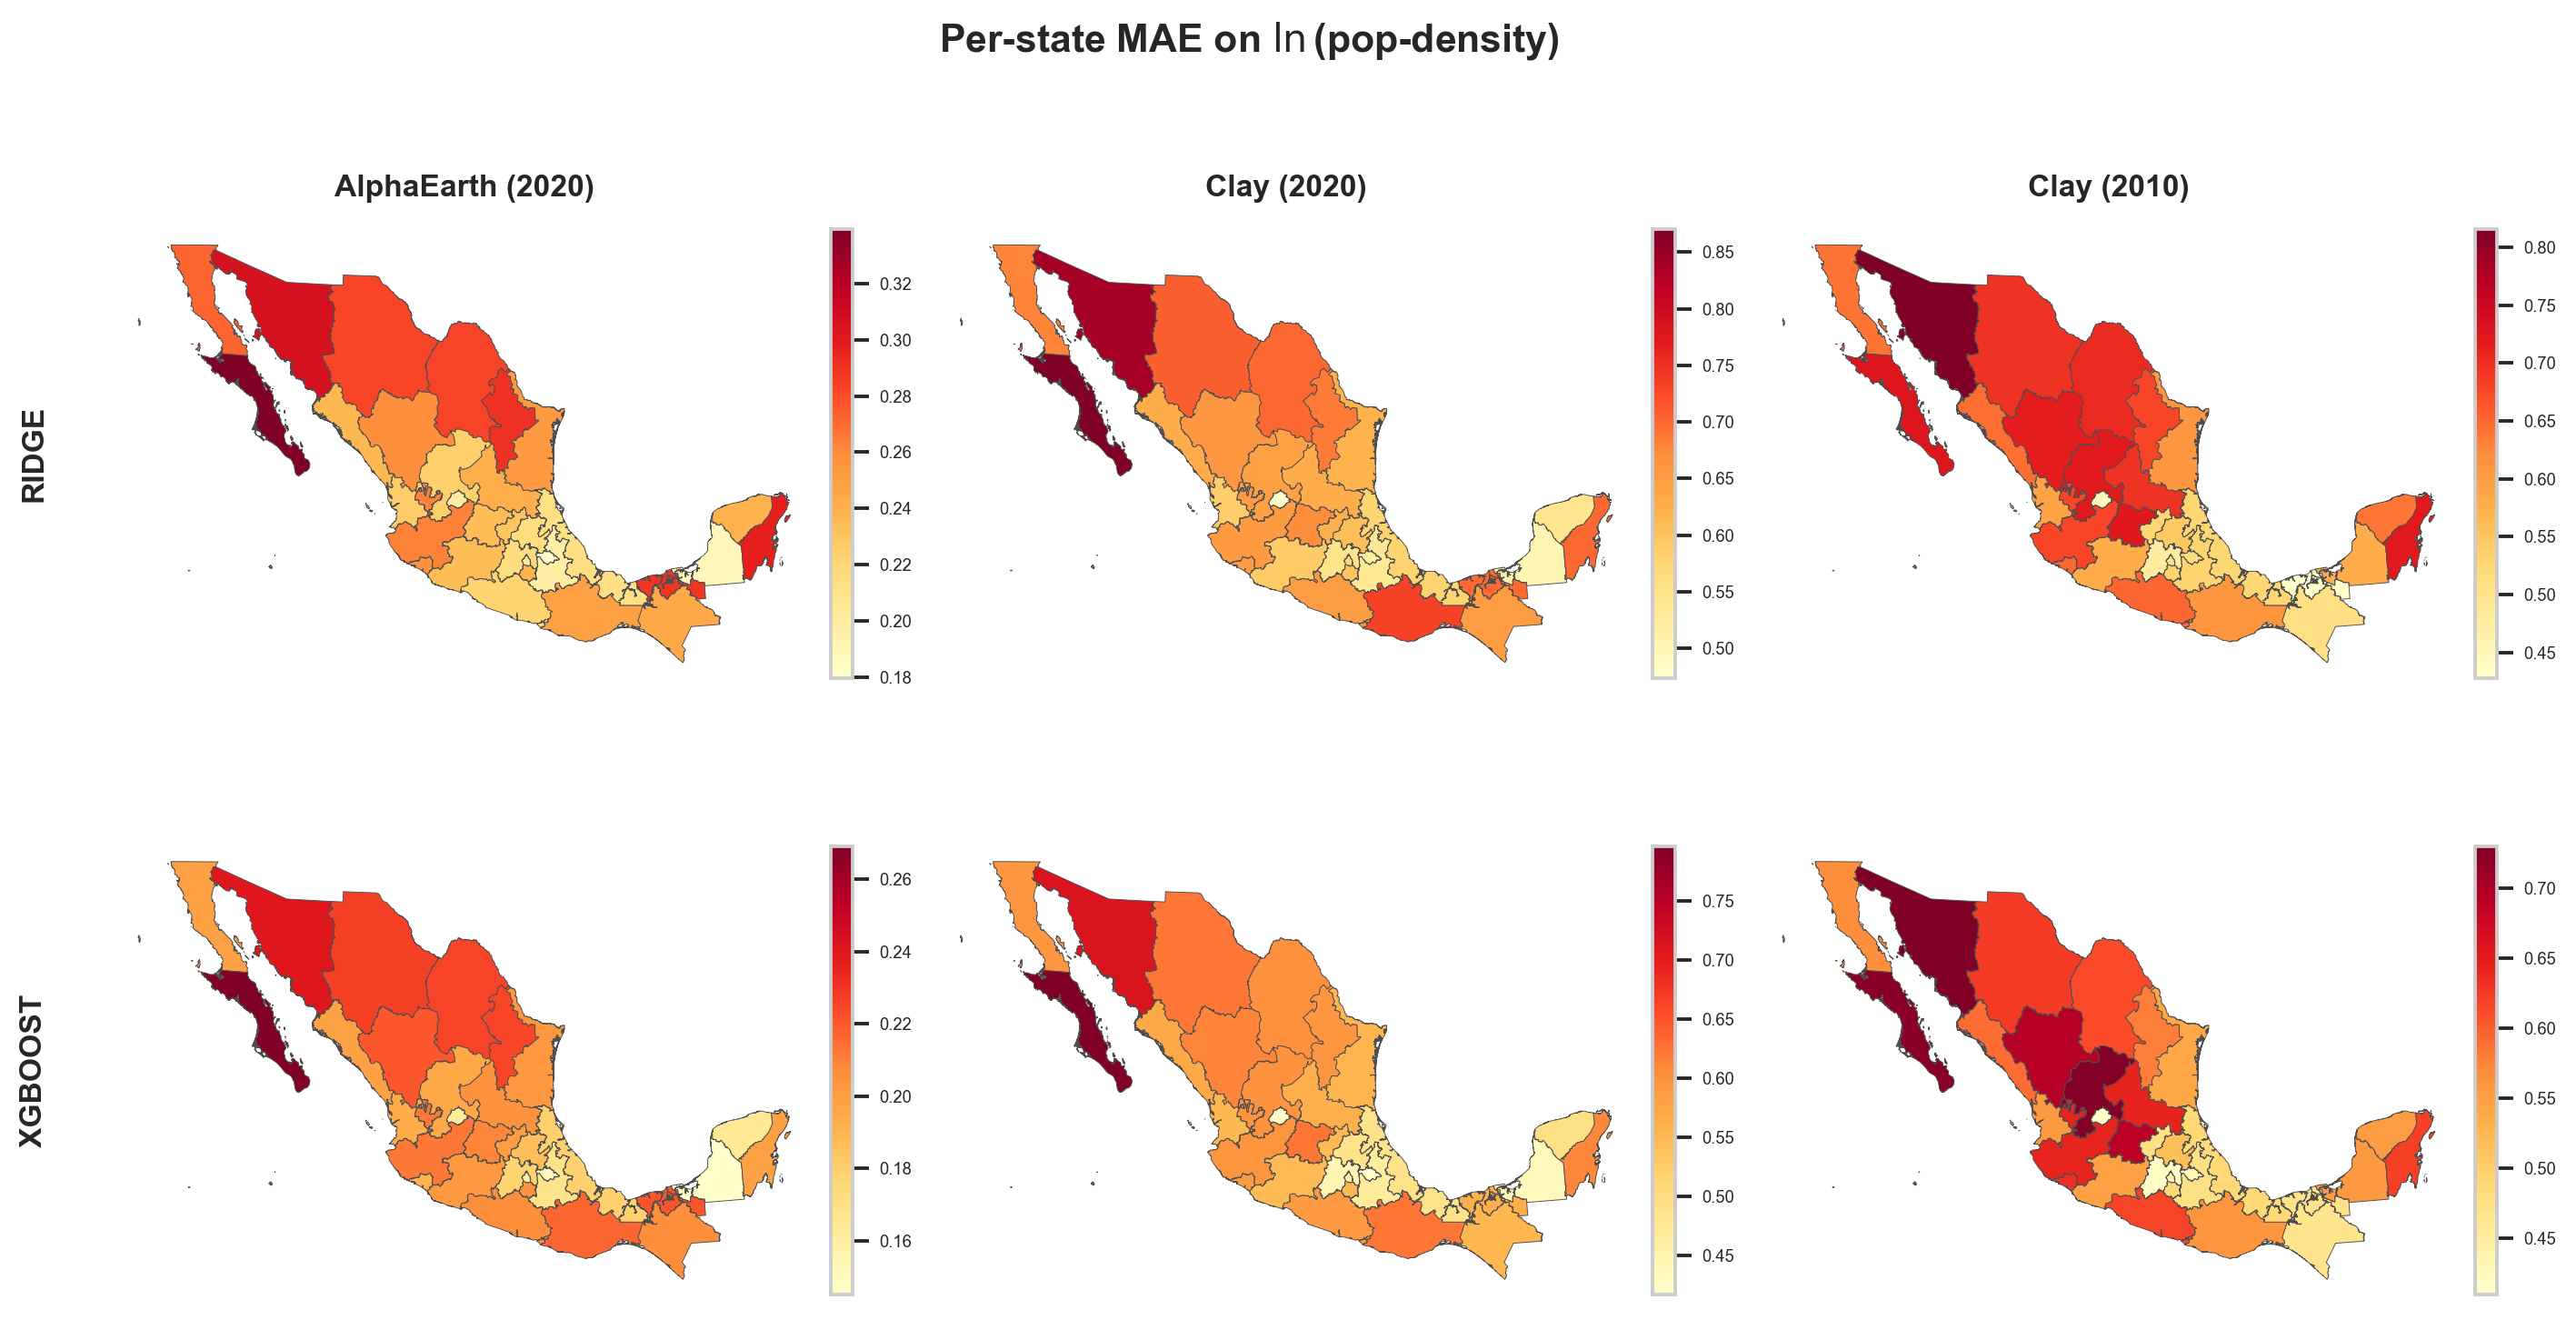
\includegraphics[width=\linewidth]{figs/spatial_state_mae.png}
  \caption{State choropleths of polygon-scale out-of-fold MAE on $\ln(y)$ (same layout as Figure~\ref{fig:spatial_state_r2}). Darker shading indicates higher error.}
  \label{fig:spatial_state_mae}
\end{figure}

\begin{figure}[htbp]
  \centering
  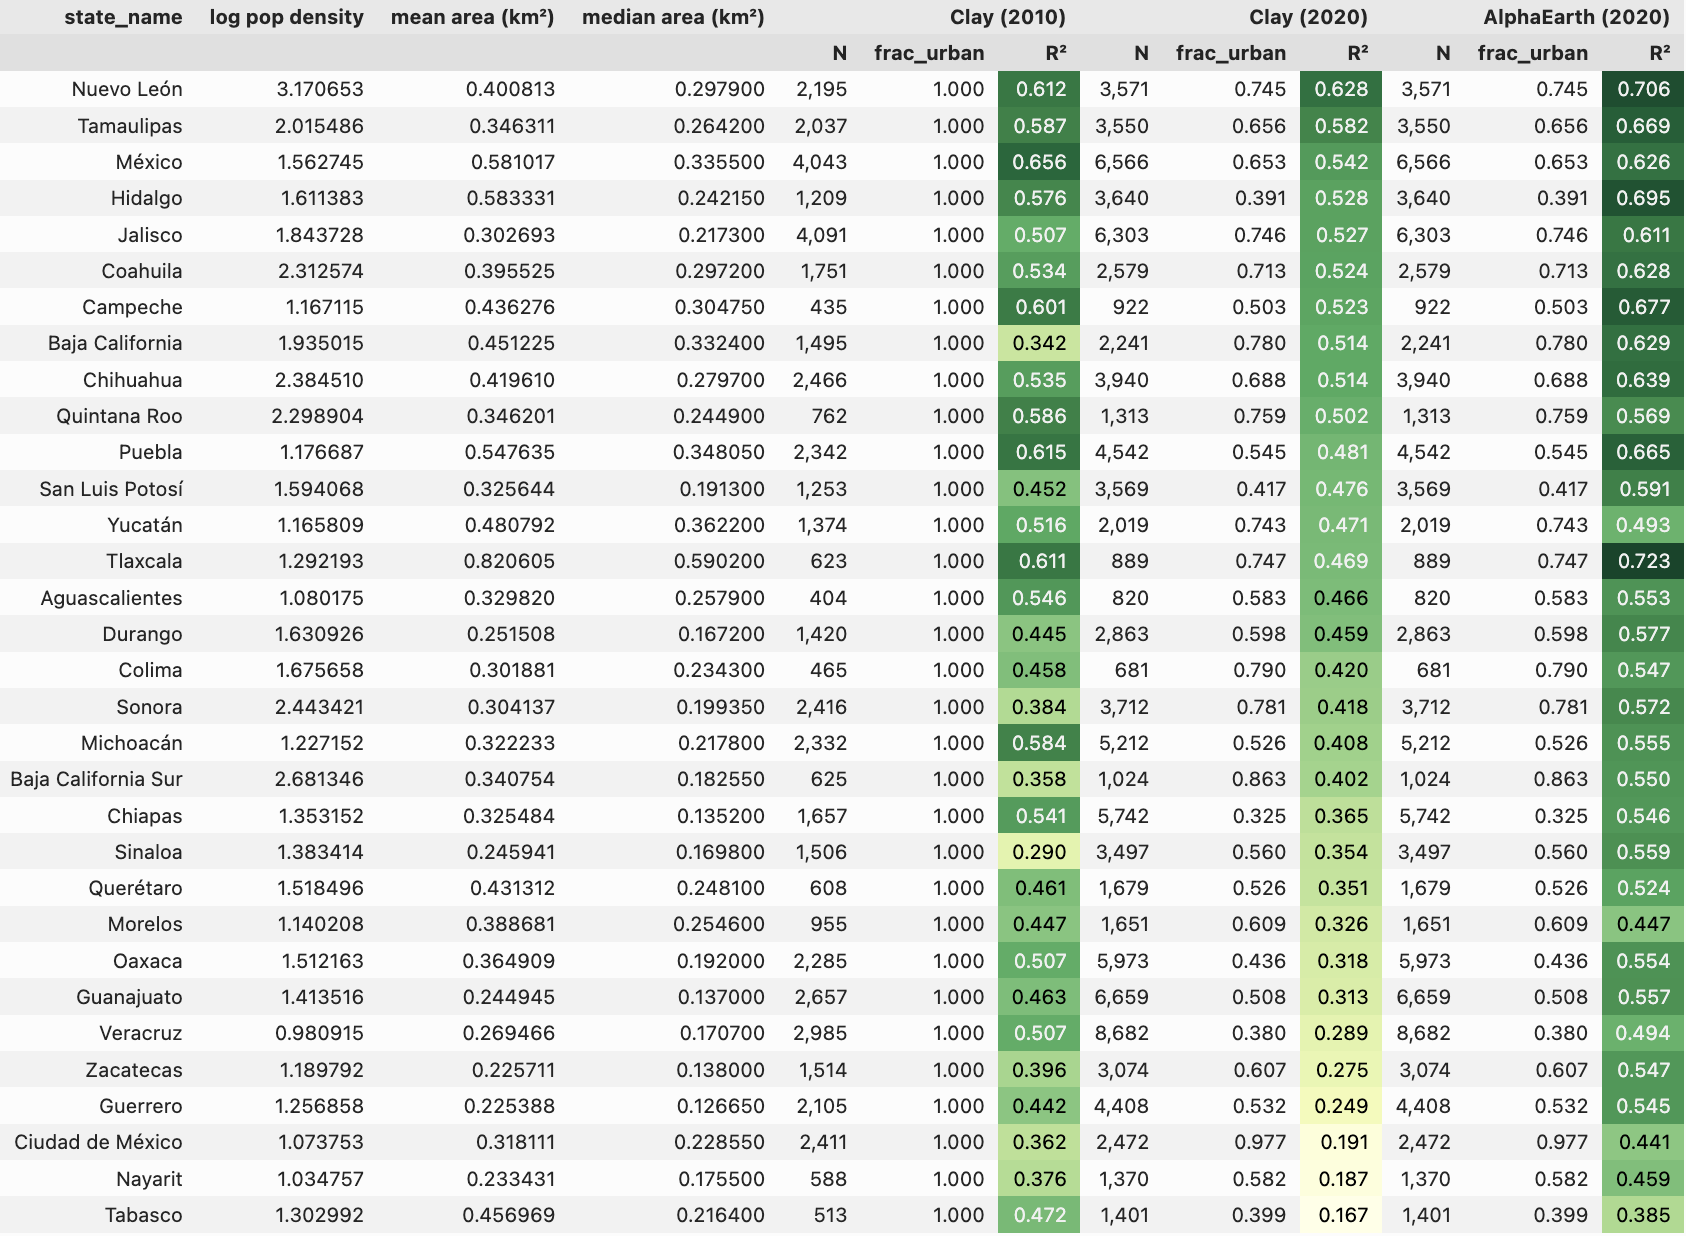
\includegraphics[width=\linewidth]{figs/statebystate_table.png}
  \caption{State-by-state ridge out-of-fold performance on $\ln(y)$ (same head as Figure~\ref{fig:spatial_state_r2}): polygon sample size $n$, urban AGEB-length heuristic $f_{\mathrm{urb}}$, and $R^2$ under Clay (2010), Clay (2020), and AlphaEarth (2020), with single-column $\mathrm{Var}(y)$, mean area, and median area (km$^2$). Exported raster from the cross-model comparison notebook.}
  \label{fig:statebystate_table}
\end{figure}

\clearpage

\section{Drivers of State-Level Performance Differences Figures}
\label{appendix:drivers}

This appendix records the comprehensive data characteristics table and individual scatterplots of $R^2$ performance against key spatial and statistical drivers (Section \ref{subsec:drivers_state} of the main text).

\begin{figure}[htbp]
  \centering
  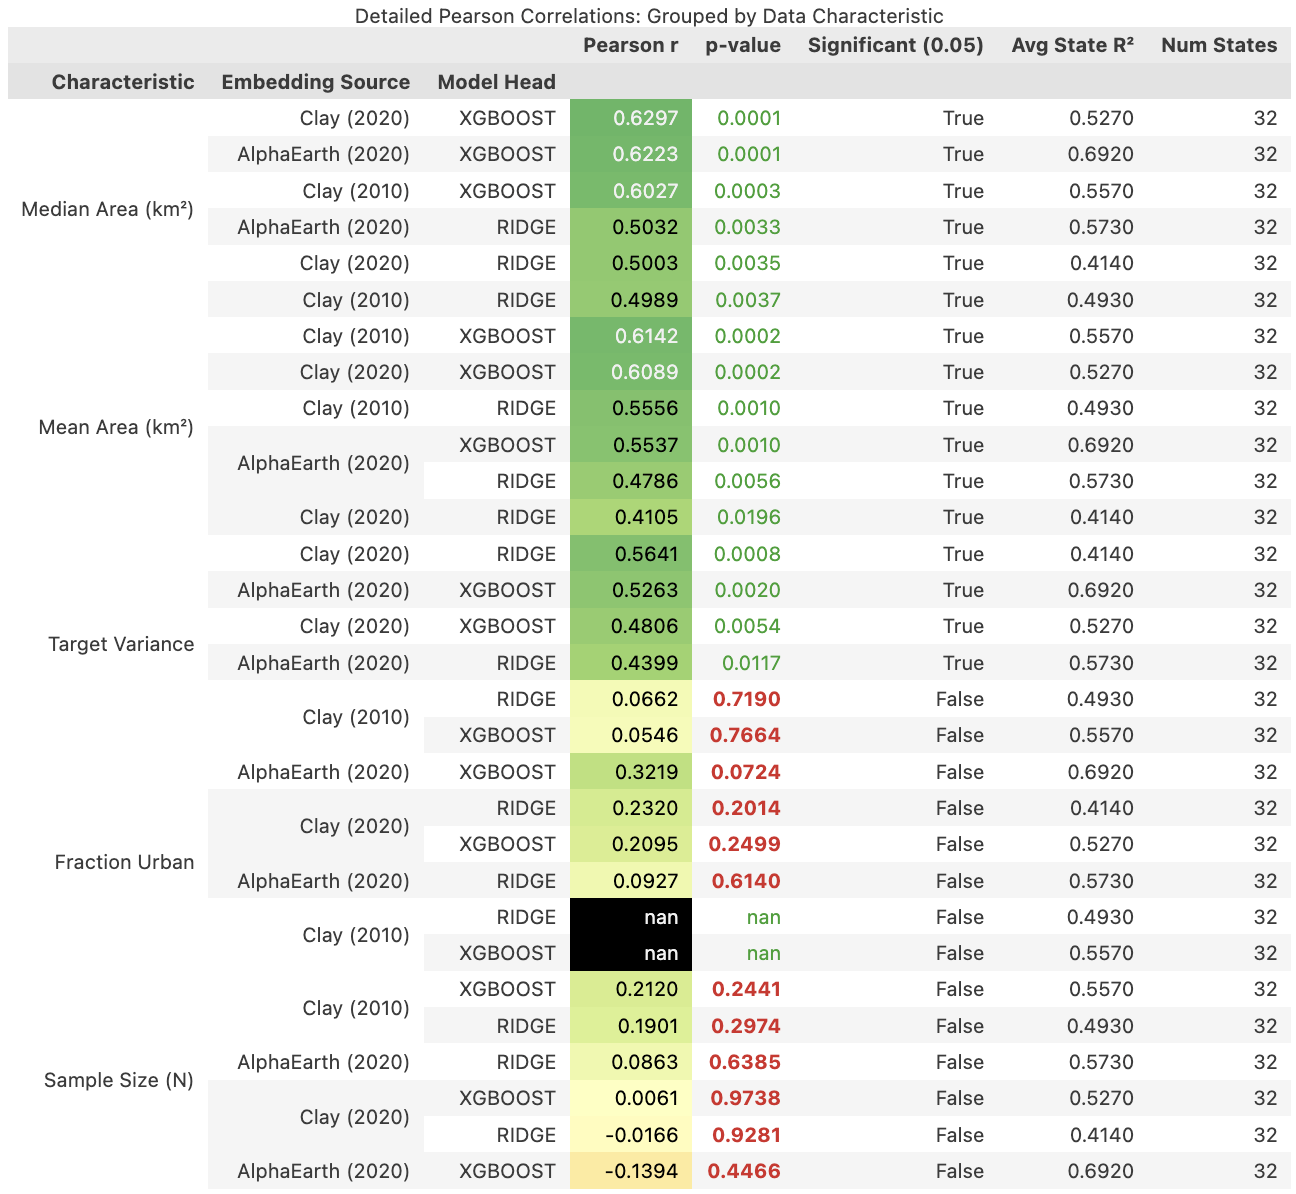
\includegraphics[width=\linewidth]{figs/full_table_data_characteristics_importance.png}
  \caption{State-level $R^2$ and various data characteristics across all model configurations.  Exported raster from the cross-model comparison notebook.}
  \label{tab:full_table_data_characteristics_importance}
\end{figure}

\begin{figure}[htbp]
  \centering
  \begin{subfigure}{\linewidth}
    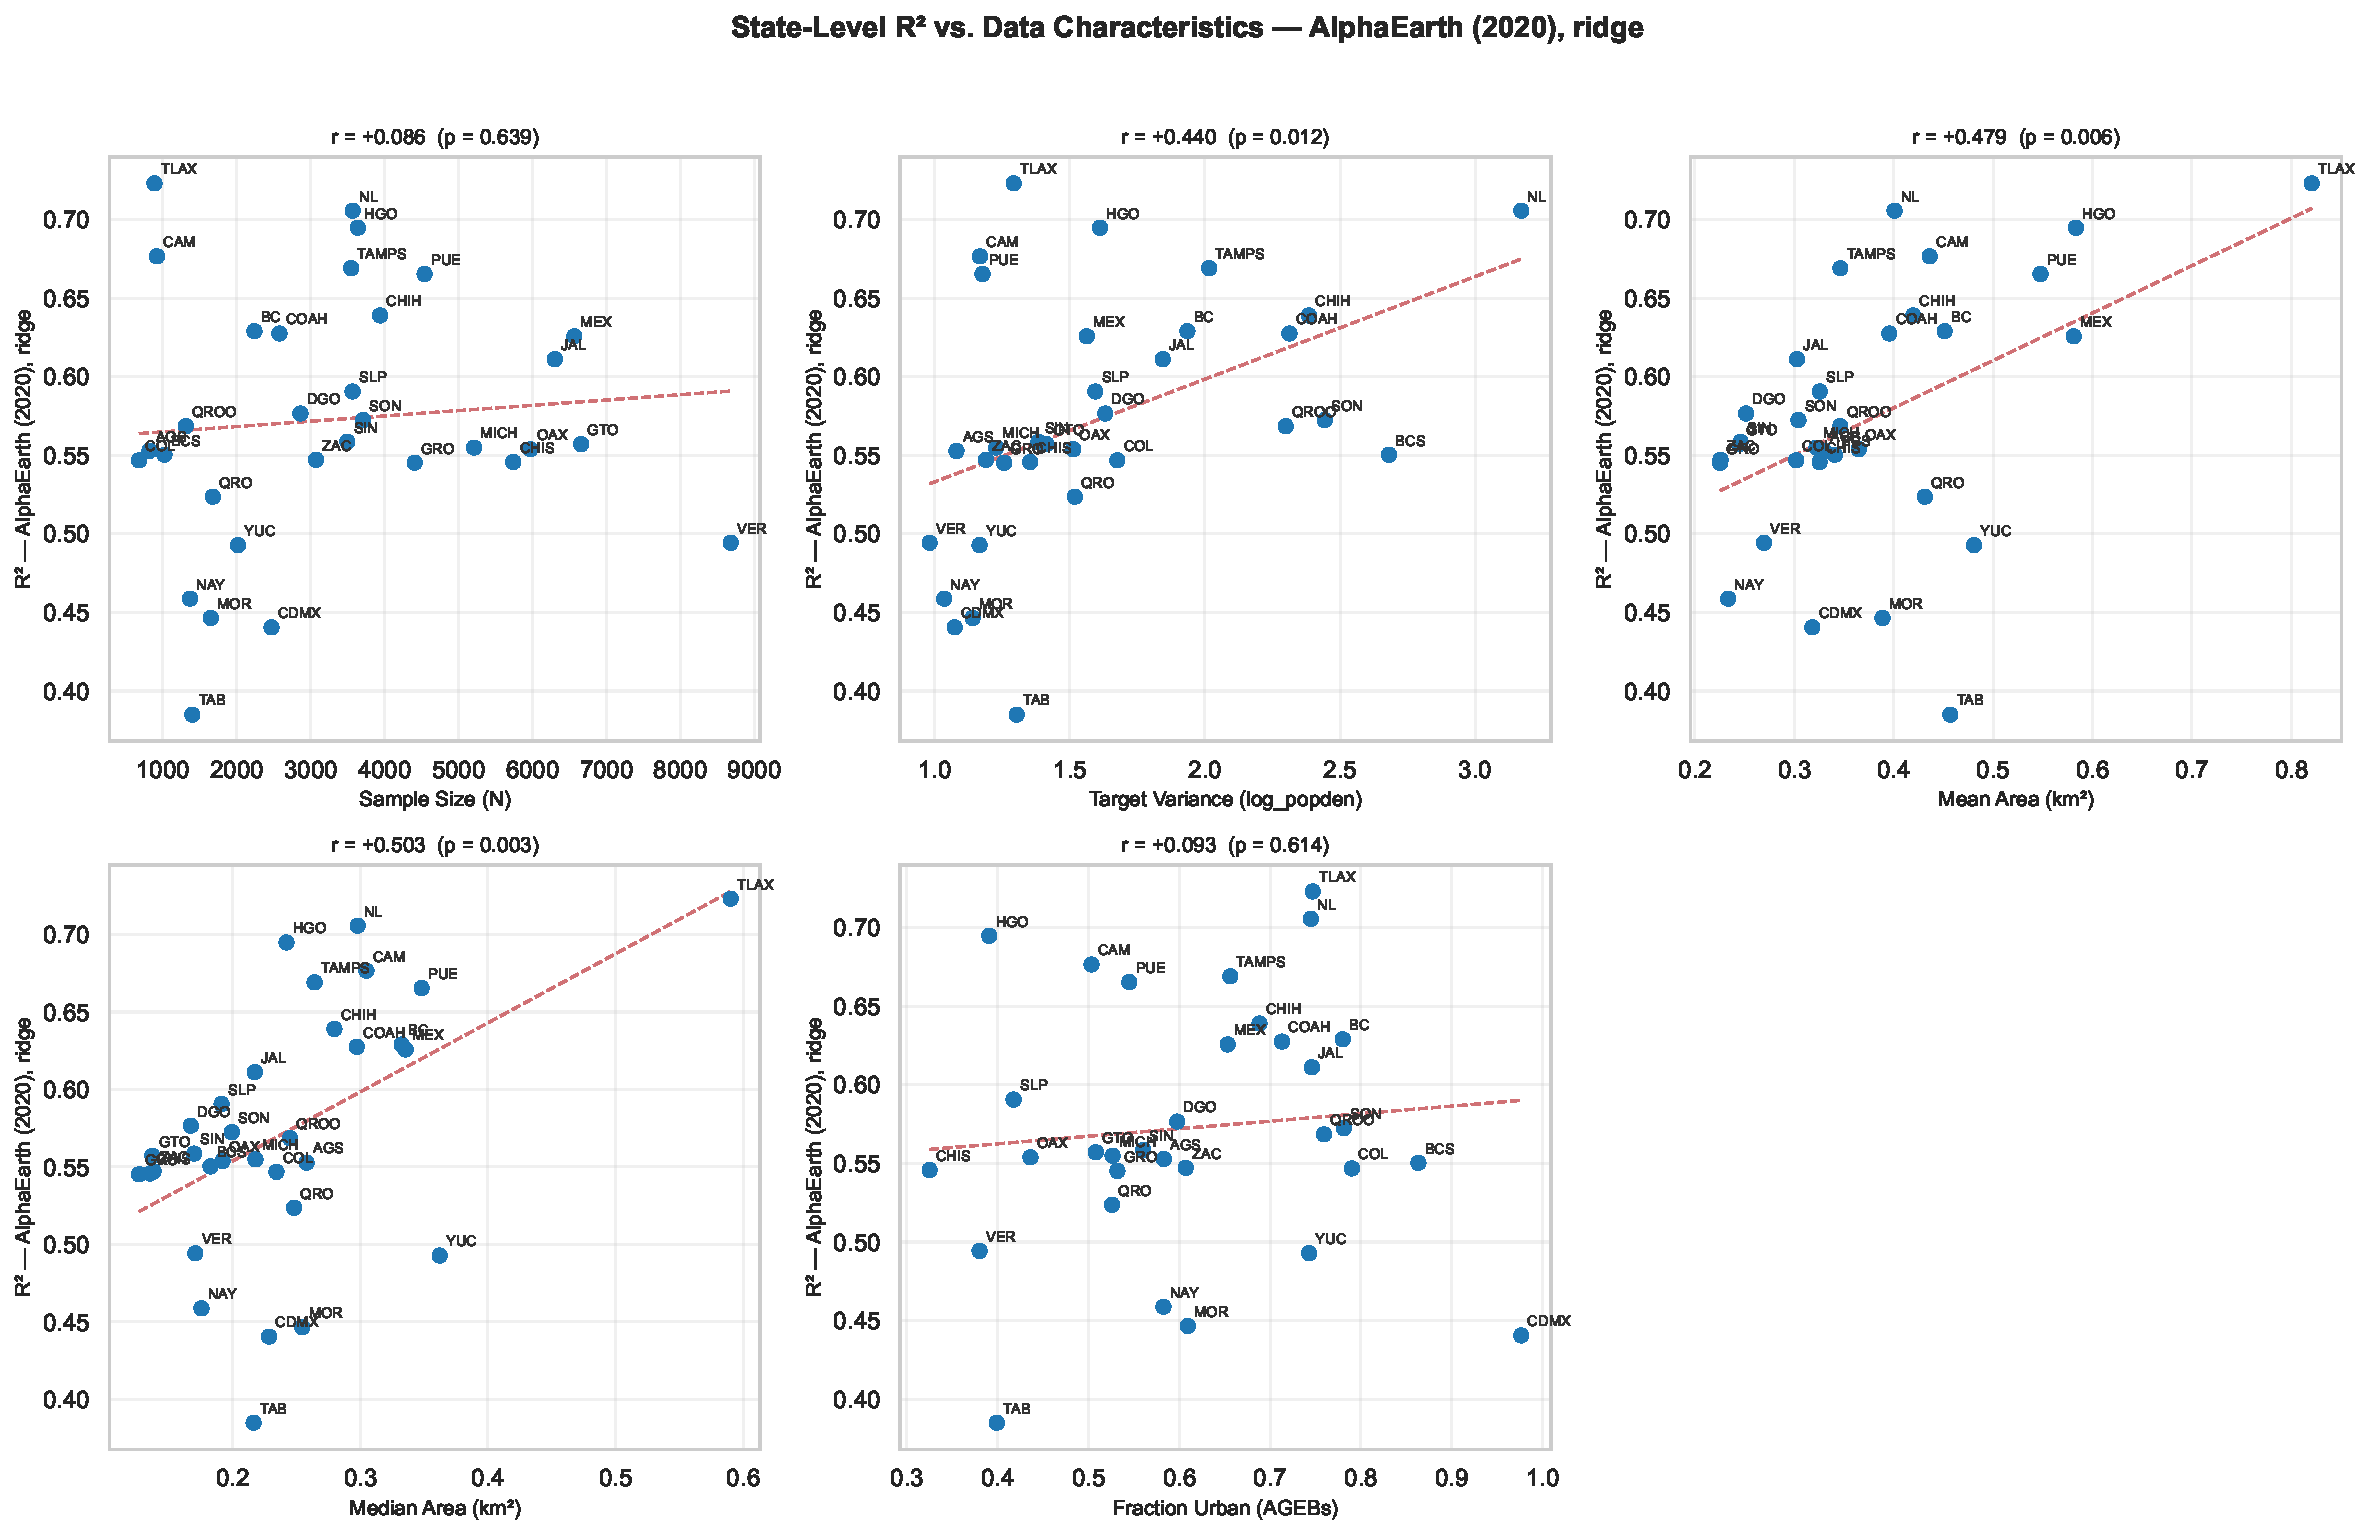
\includegraphics[width=\linewidth]{figs/state_r2_vs_characteristics_alphaearth2020_ridge.pdf}
    \caption{AlphaEarth, 2020 labels, ridge head.}
    \label{fig:state_r2_drivers_alphaearth_2020_ridge}
  \end{subfigure}
  \vspace{1em}
  \begin{subfigure}{\linewidth}
    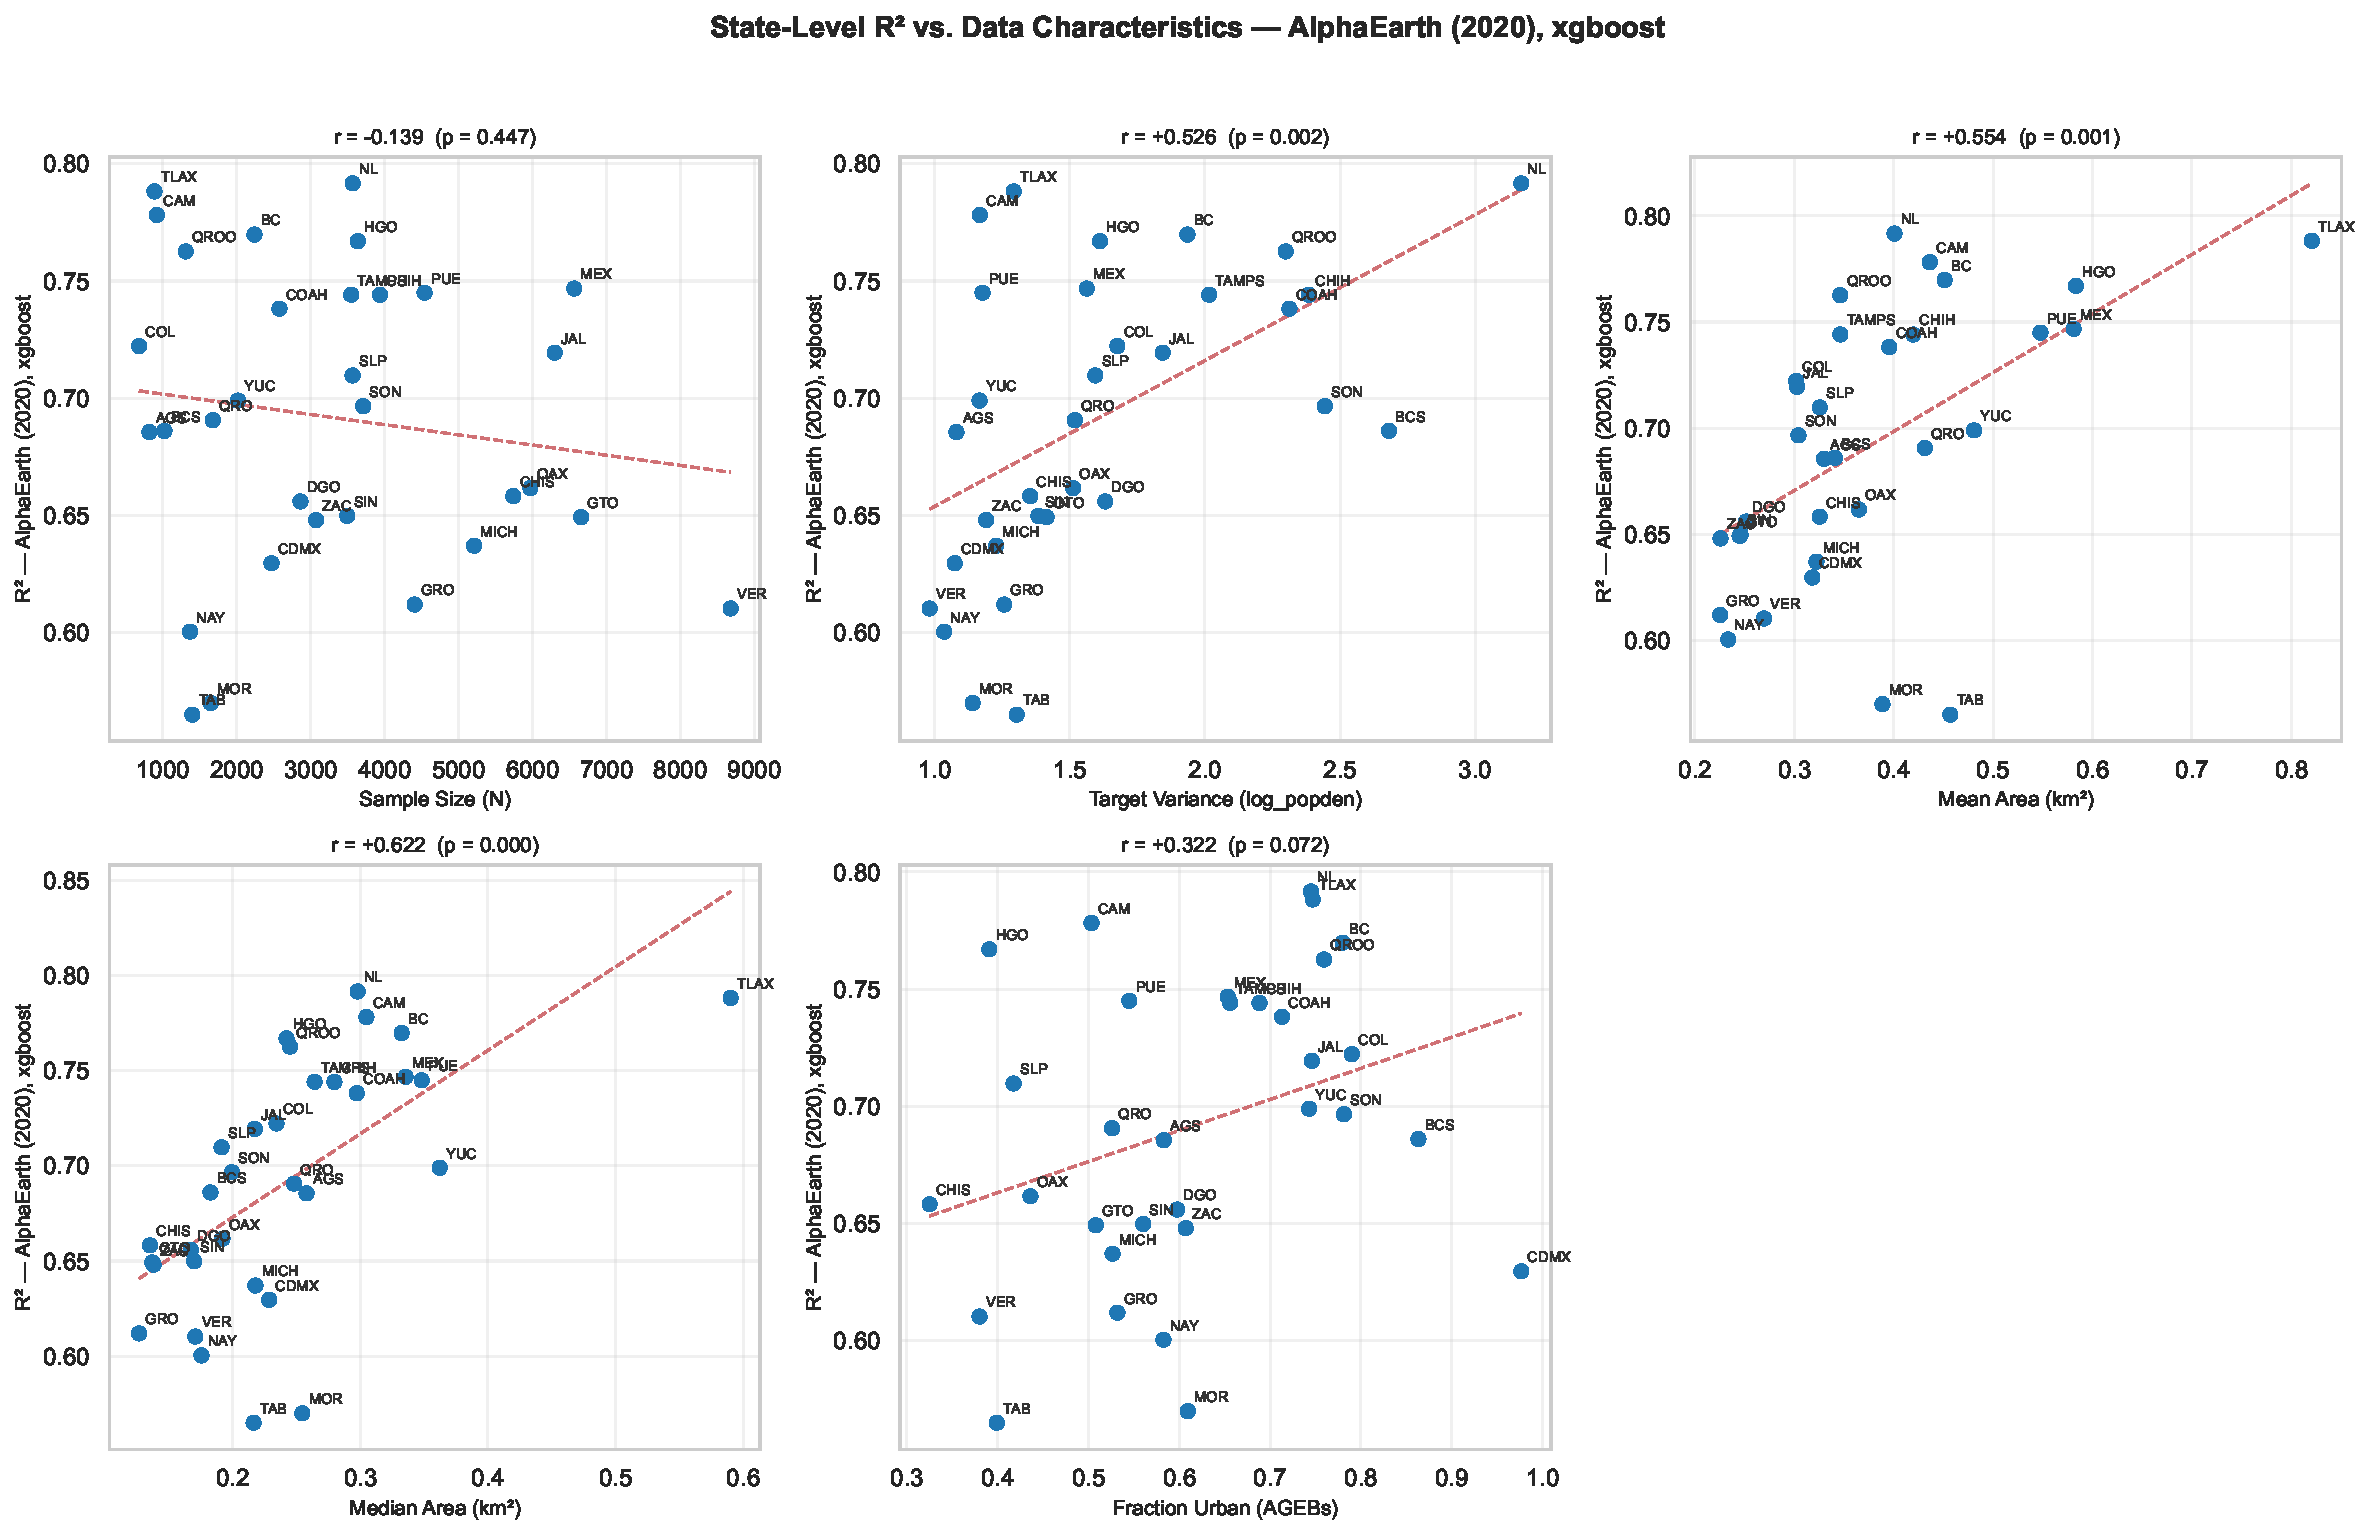
\includegraphics[width=\linewidth]{figs/state_r2_vs_characteristics_alphaearth2020_xgboost.pdf}
    \caption{AlphaEarth, 2020 labels, XGBoost head.}
    \label{fig:state_r2_drivers_alphaearth_2020_xgboost}
  \end{subfigure}
  \caption{State-level $R^2$ plotted against data characteristics (AlphaEarth 2020). Pearson $r$ and $p$-value are annotated per panel.}
\end{figure}

\begin{figure}[htbp]
  \centering
  \begin{subfigure}{\linewidth}
    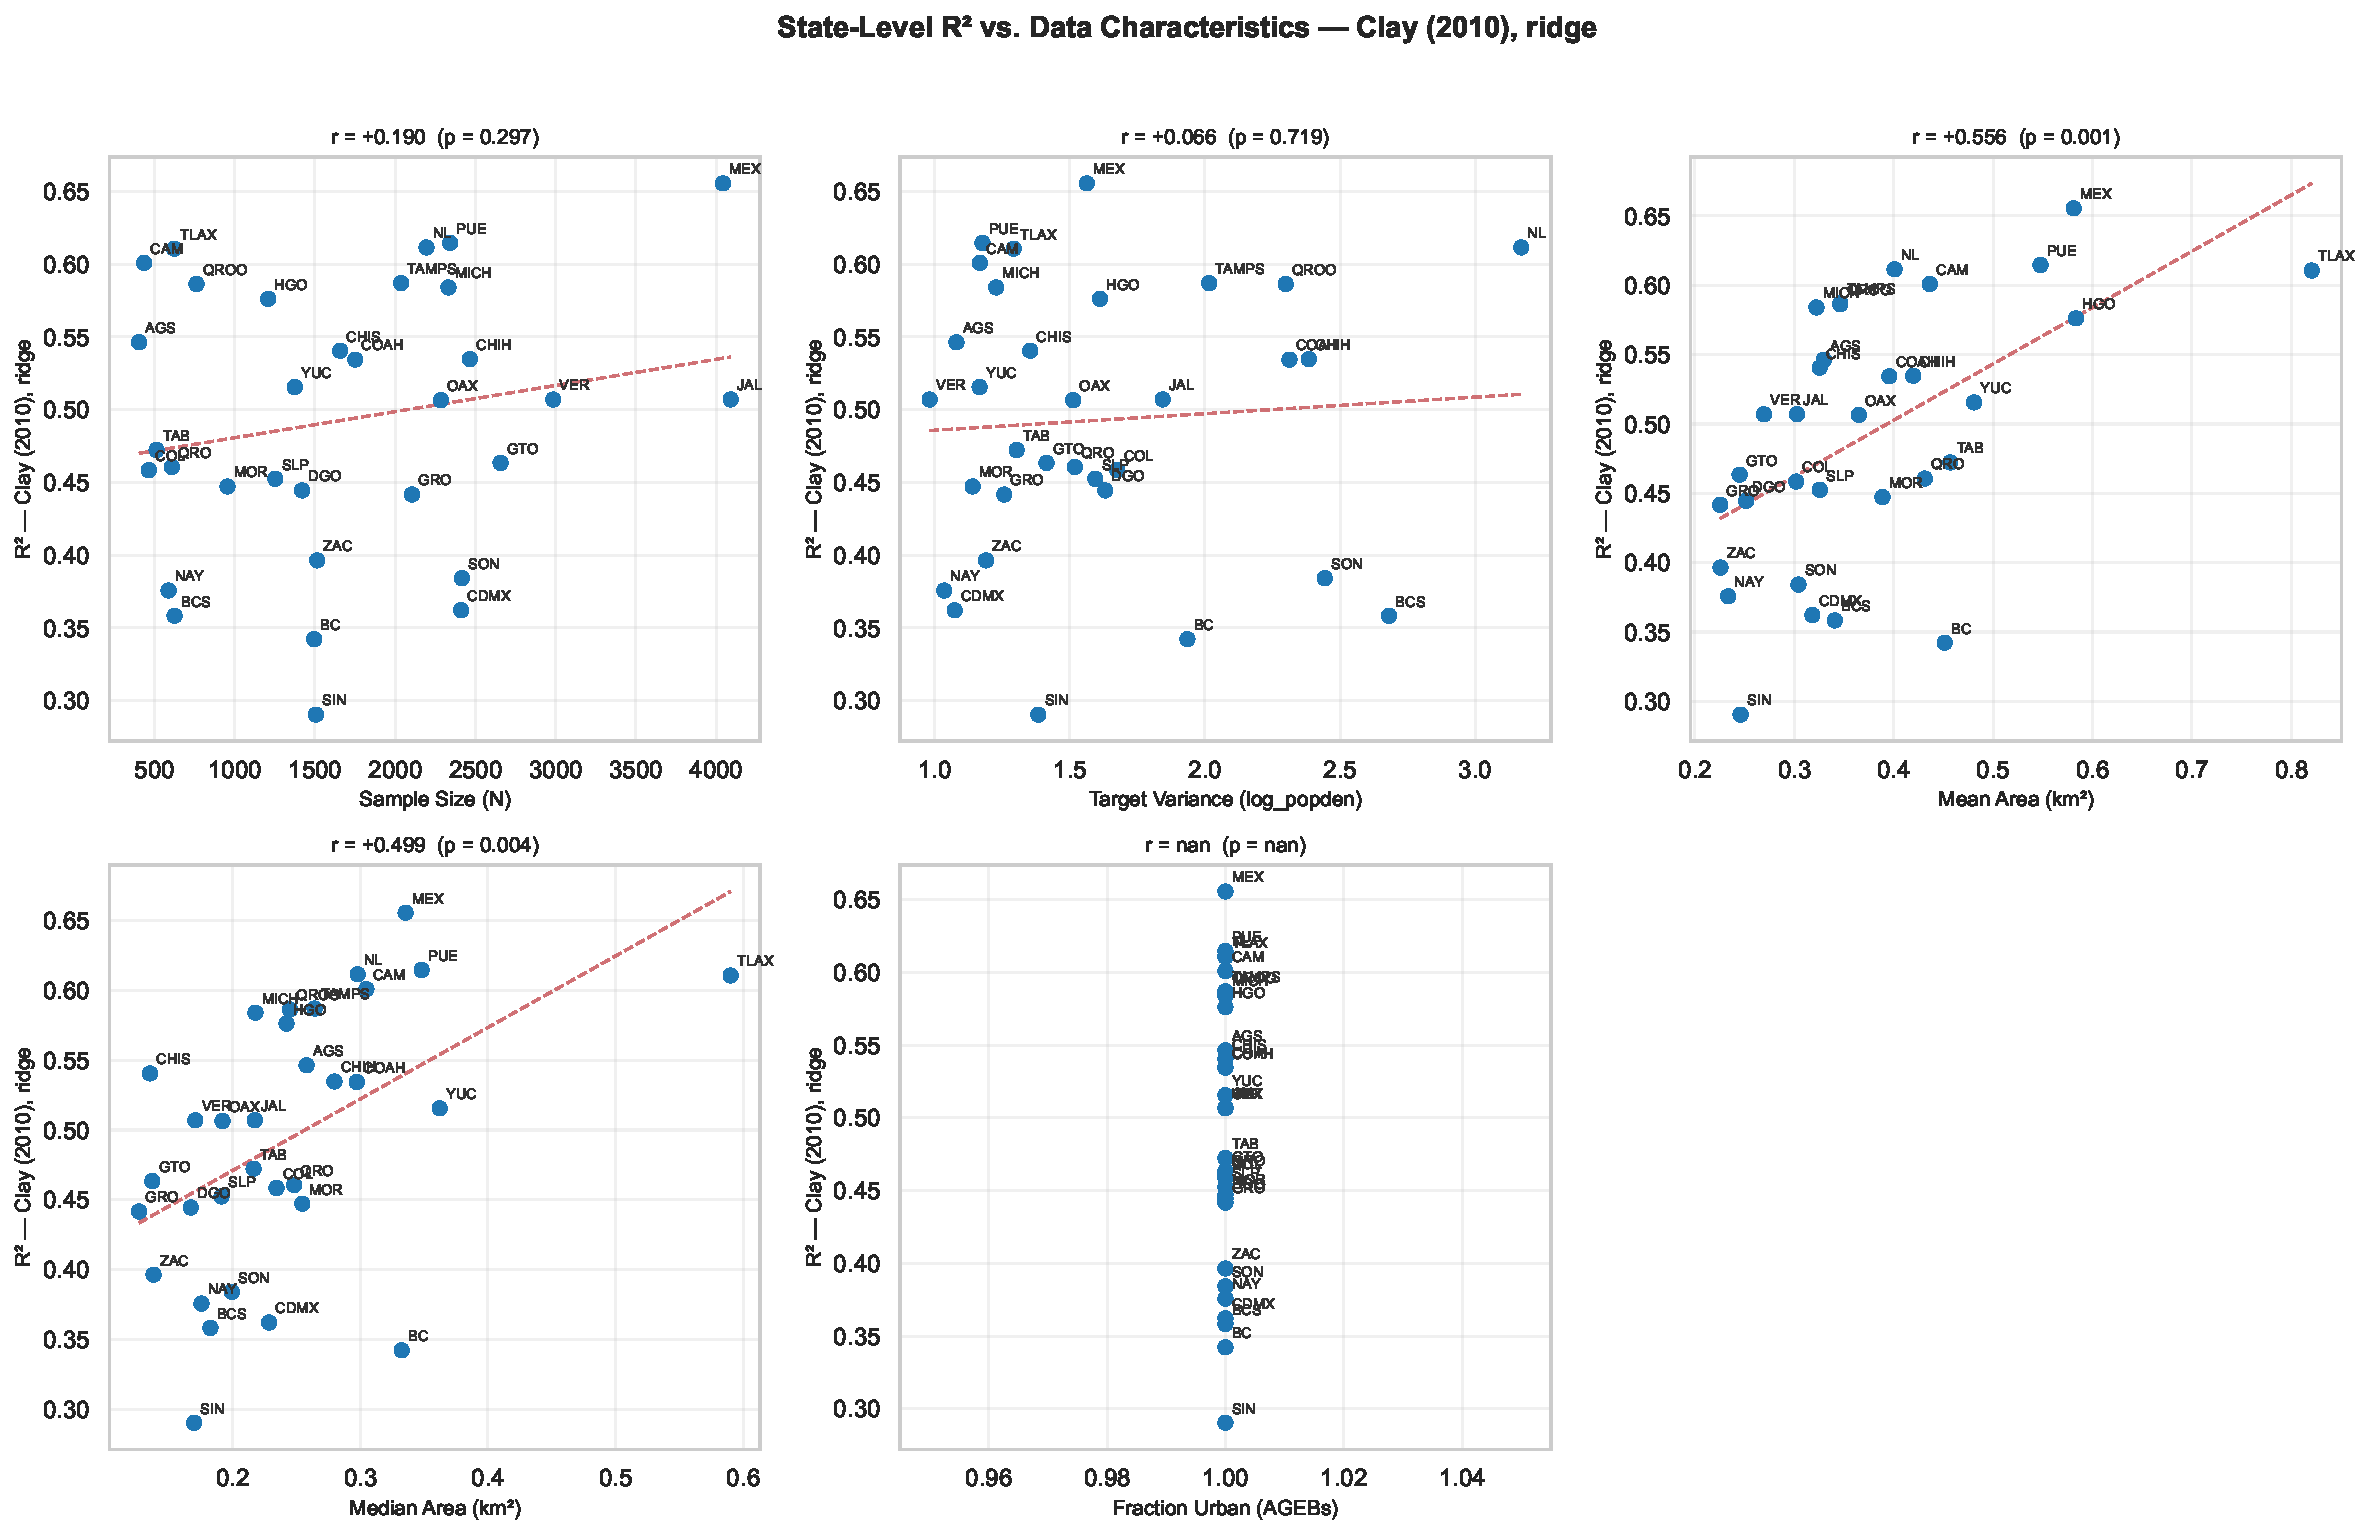
\includegraphics[width=\linewidth]{figs/state_r2_vs_characteristics_clay2010_ridge.pdf}
    \caption{Clay, 2010 labels, ridge head.}
    \label{fig:state_r2_drivers_clay_2010_ridge}
  \end{subfigure}
  \vspace{1em}
  \begin{subfigure}{\linewidth}
    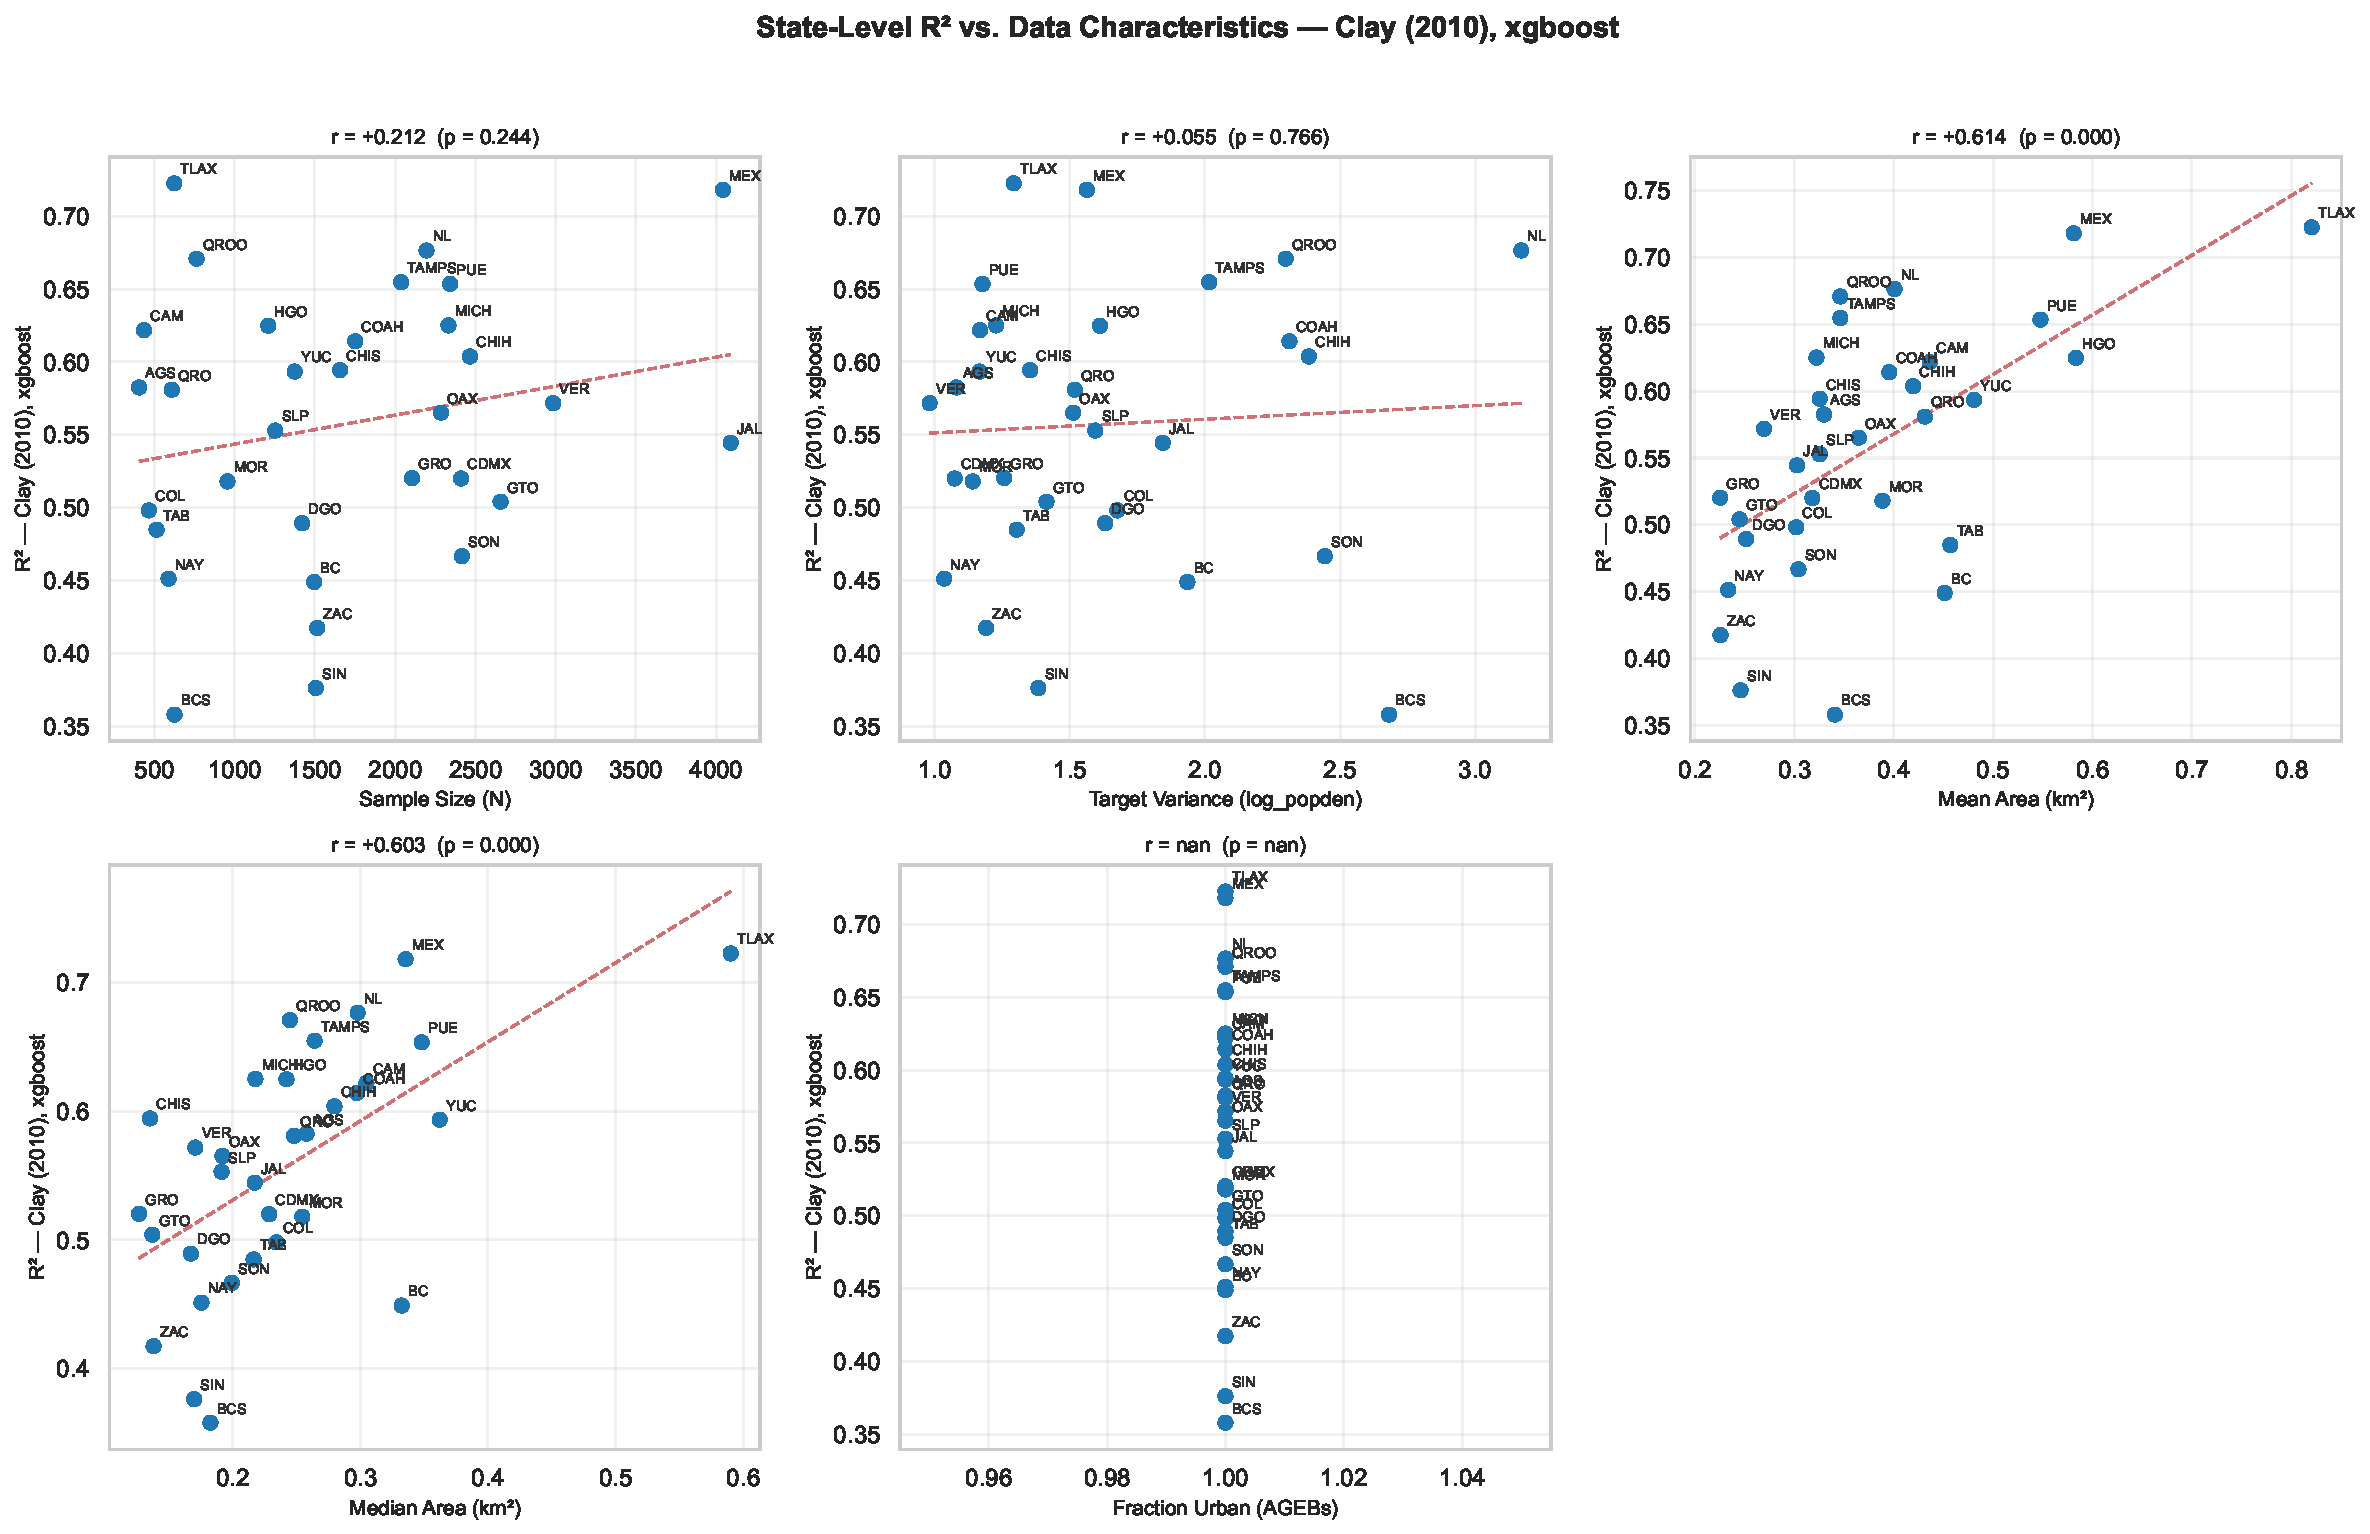
\includegraphics[width=\linewidth]{figs/state_r2_vs_characteristics_clay2010_xgboost.pdf}
    \caption{Clay, 2010 labels, XGBoost head.}
    \label{fig:state_r2_drivers_clay_2010_xgboost}
  \end{subfigure}
  \caption{State-level $R^2$ plotted against data characteristics (Clay 2010).}
\end{figure}

\begin{figure}[htbp]
  \centering
  \begin{subfigure}{\linewidth}
    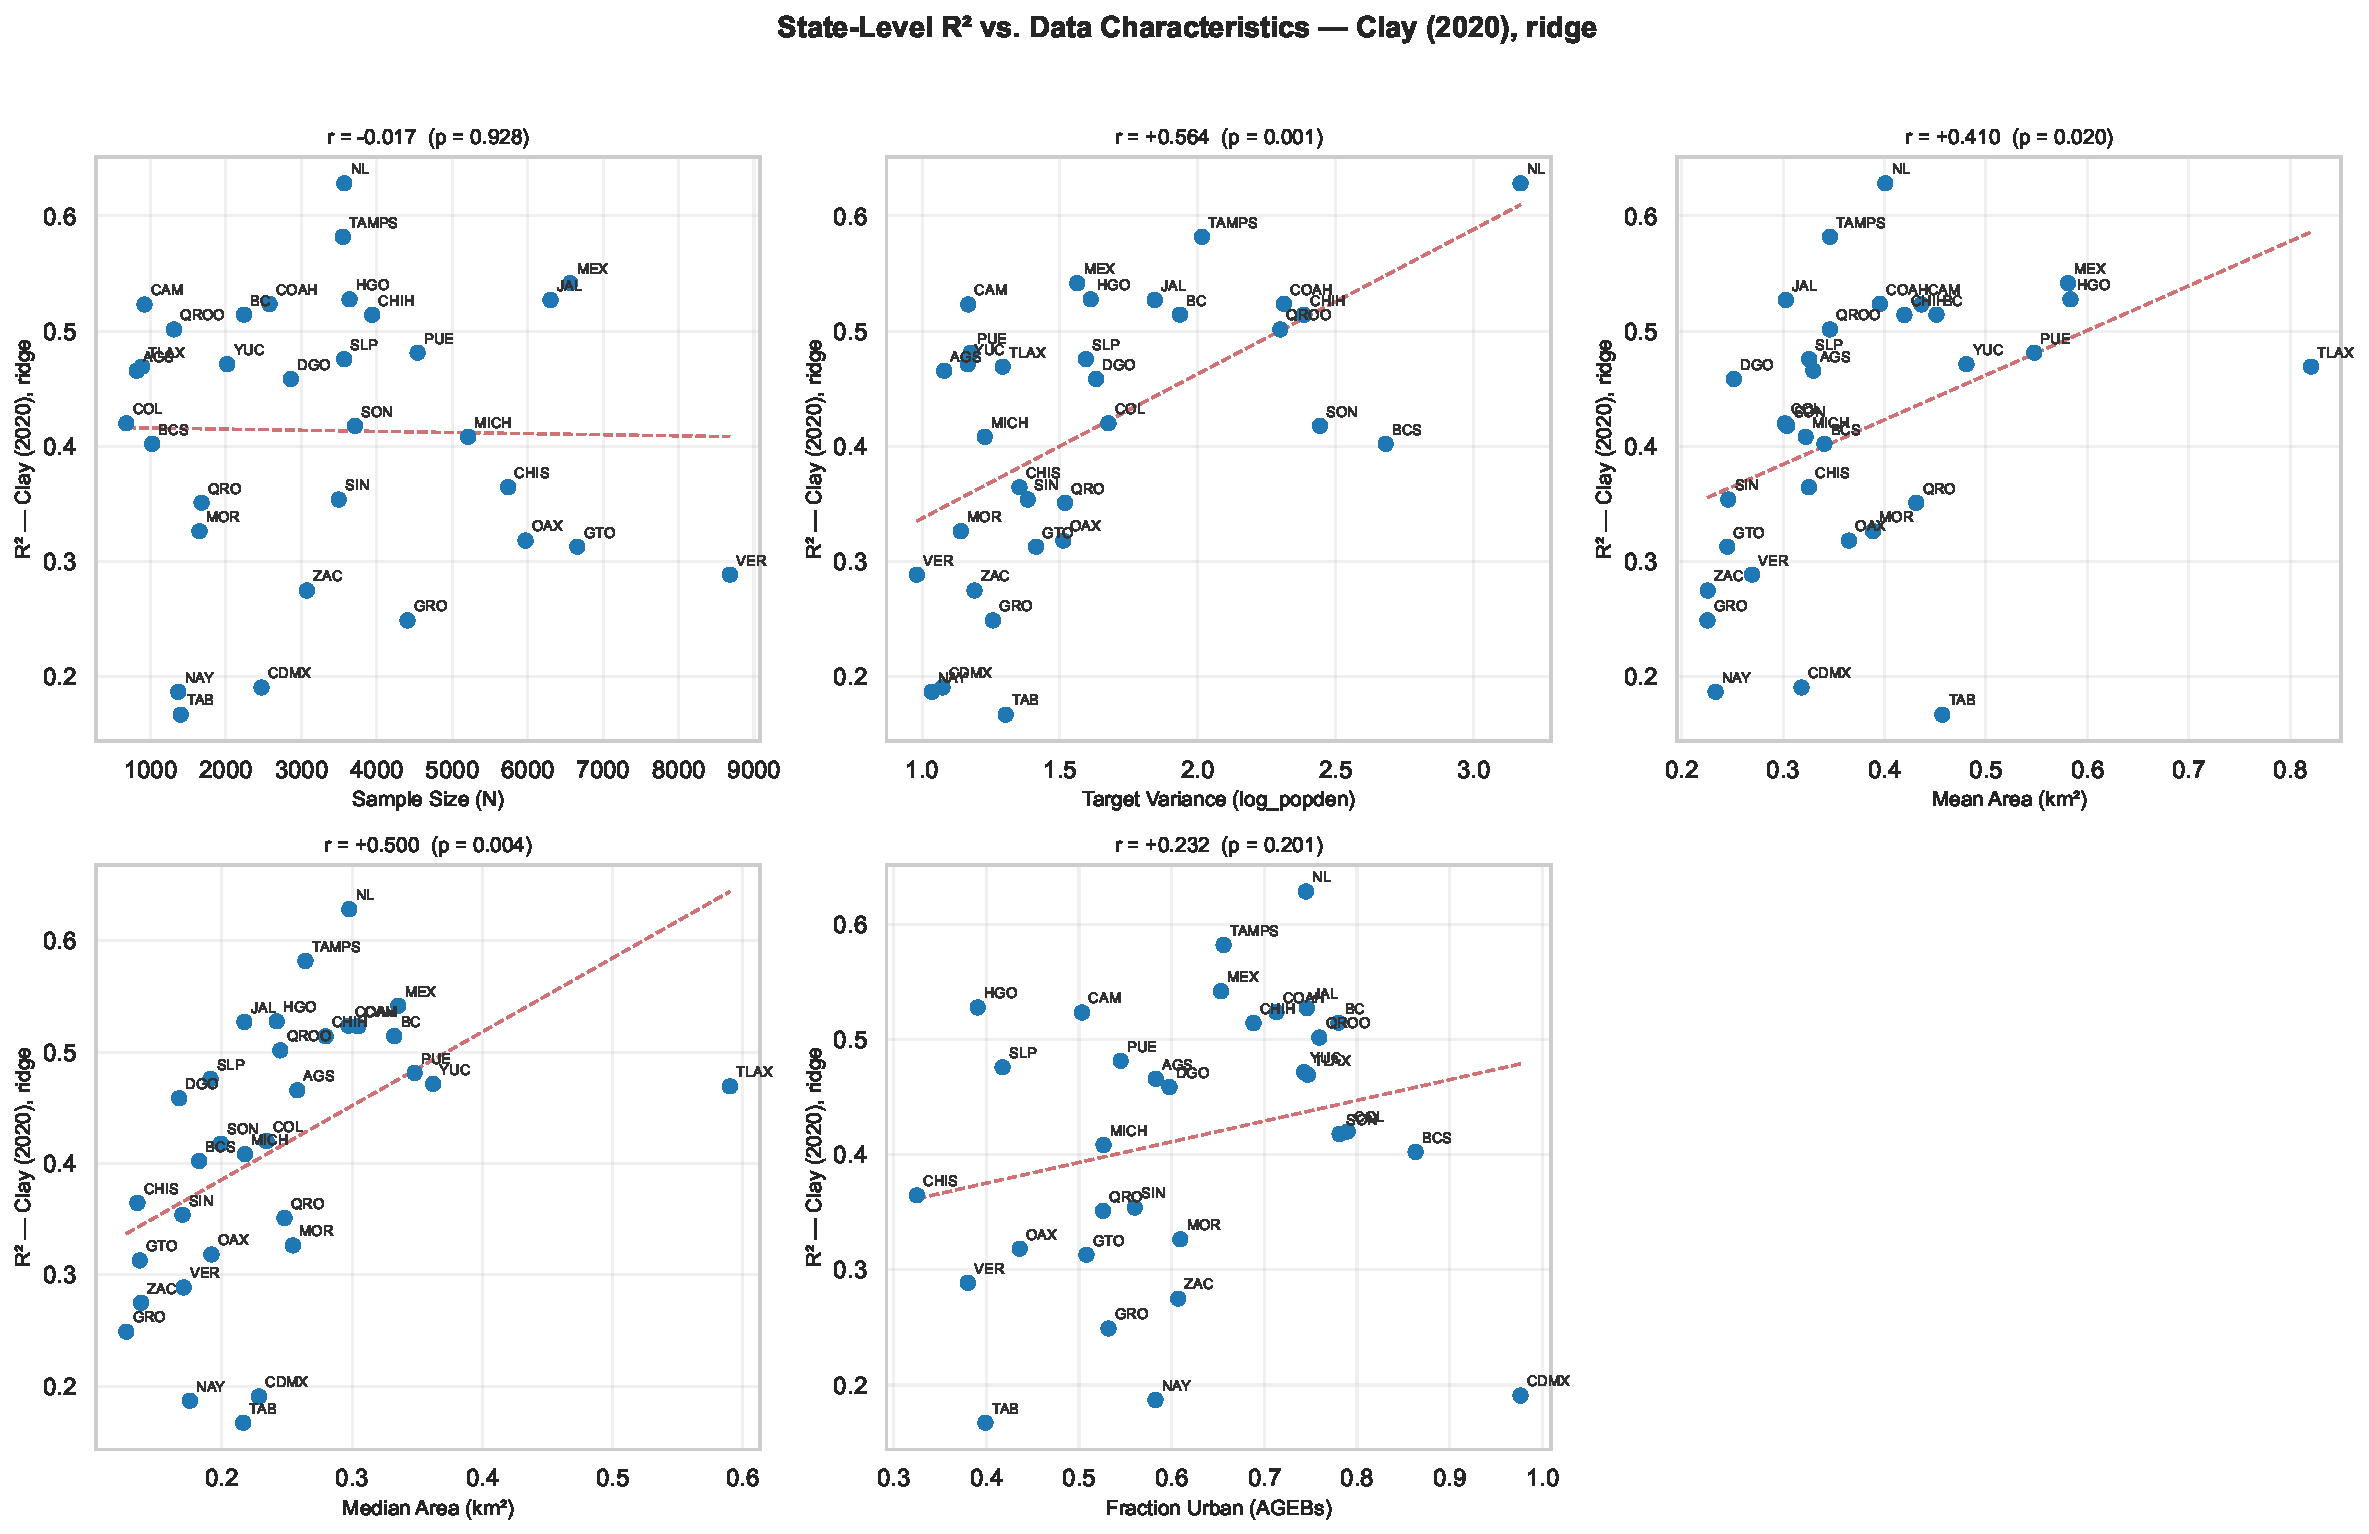
\includegraphics[width=\linewidth]{figs/state_r2_vs_characteristics_clay2020_ridge.pdf}
    \caption{Clay, 2020 labels, ridge head.}
    \label{fig:state_r2_drivers_clay_2020_ridge}
  \end{subfigure}
  \vspace{1em}
  \begin{subfigure}{\linewidth}
    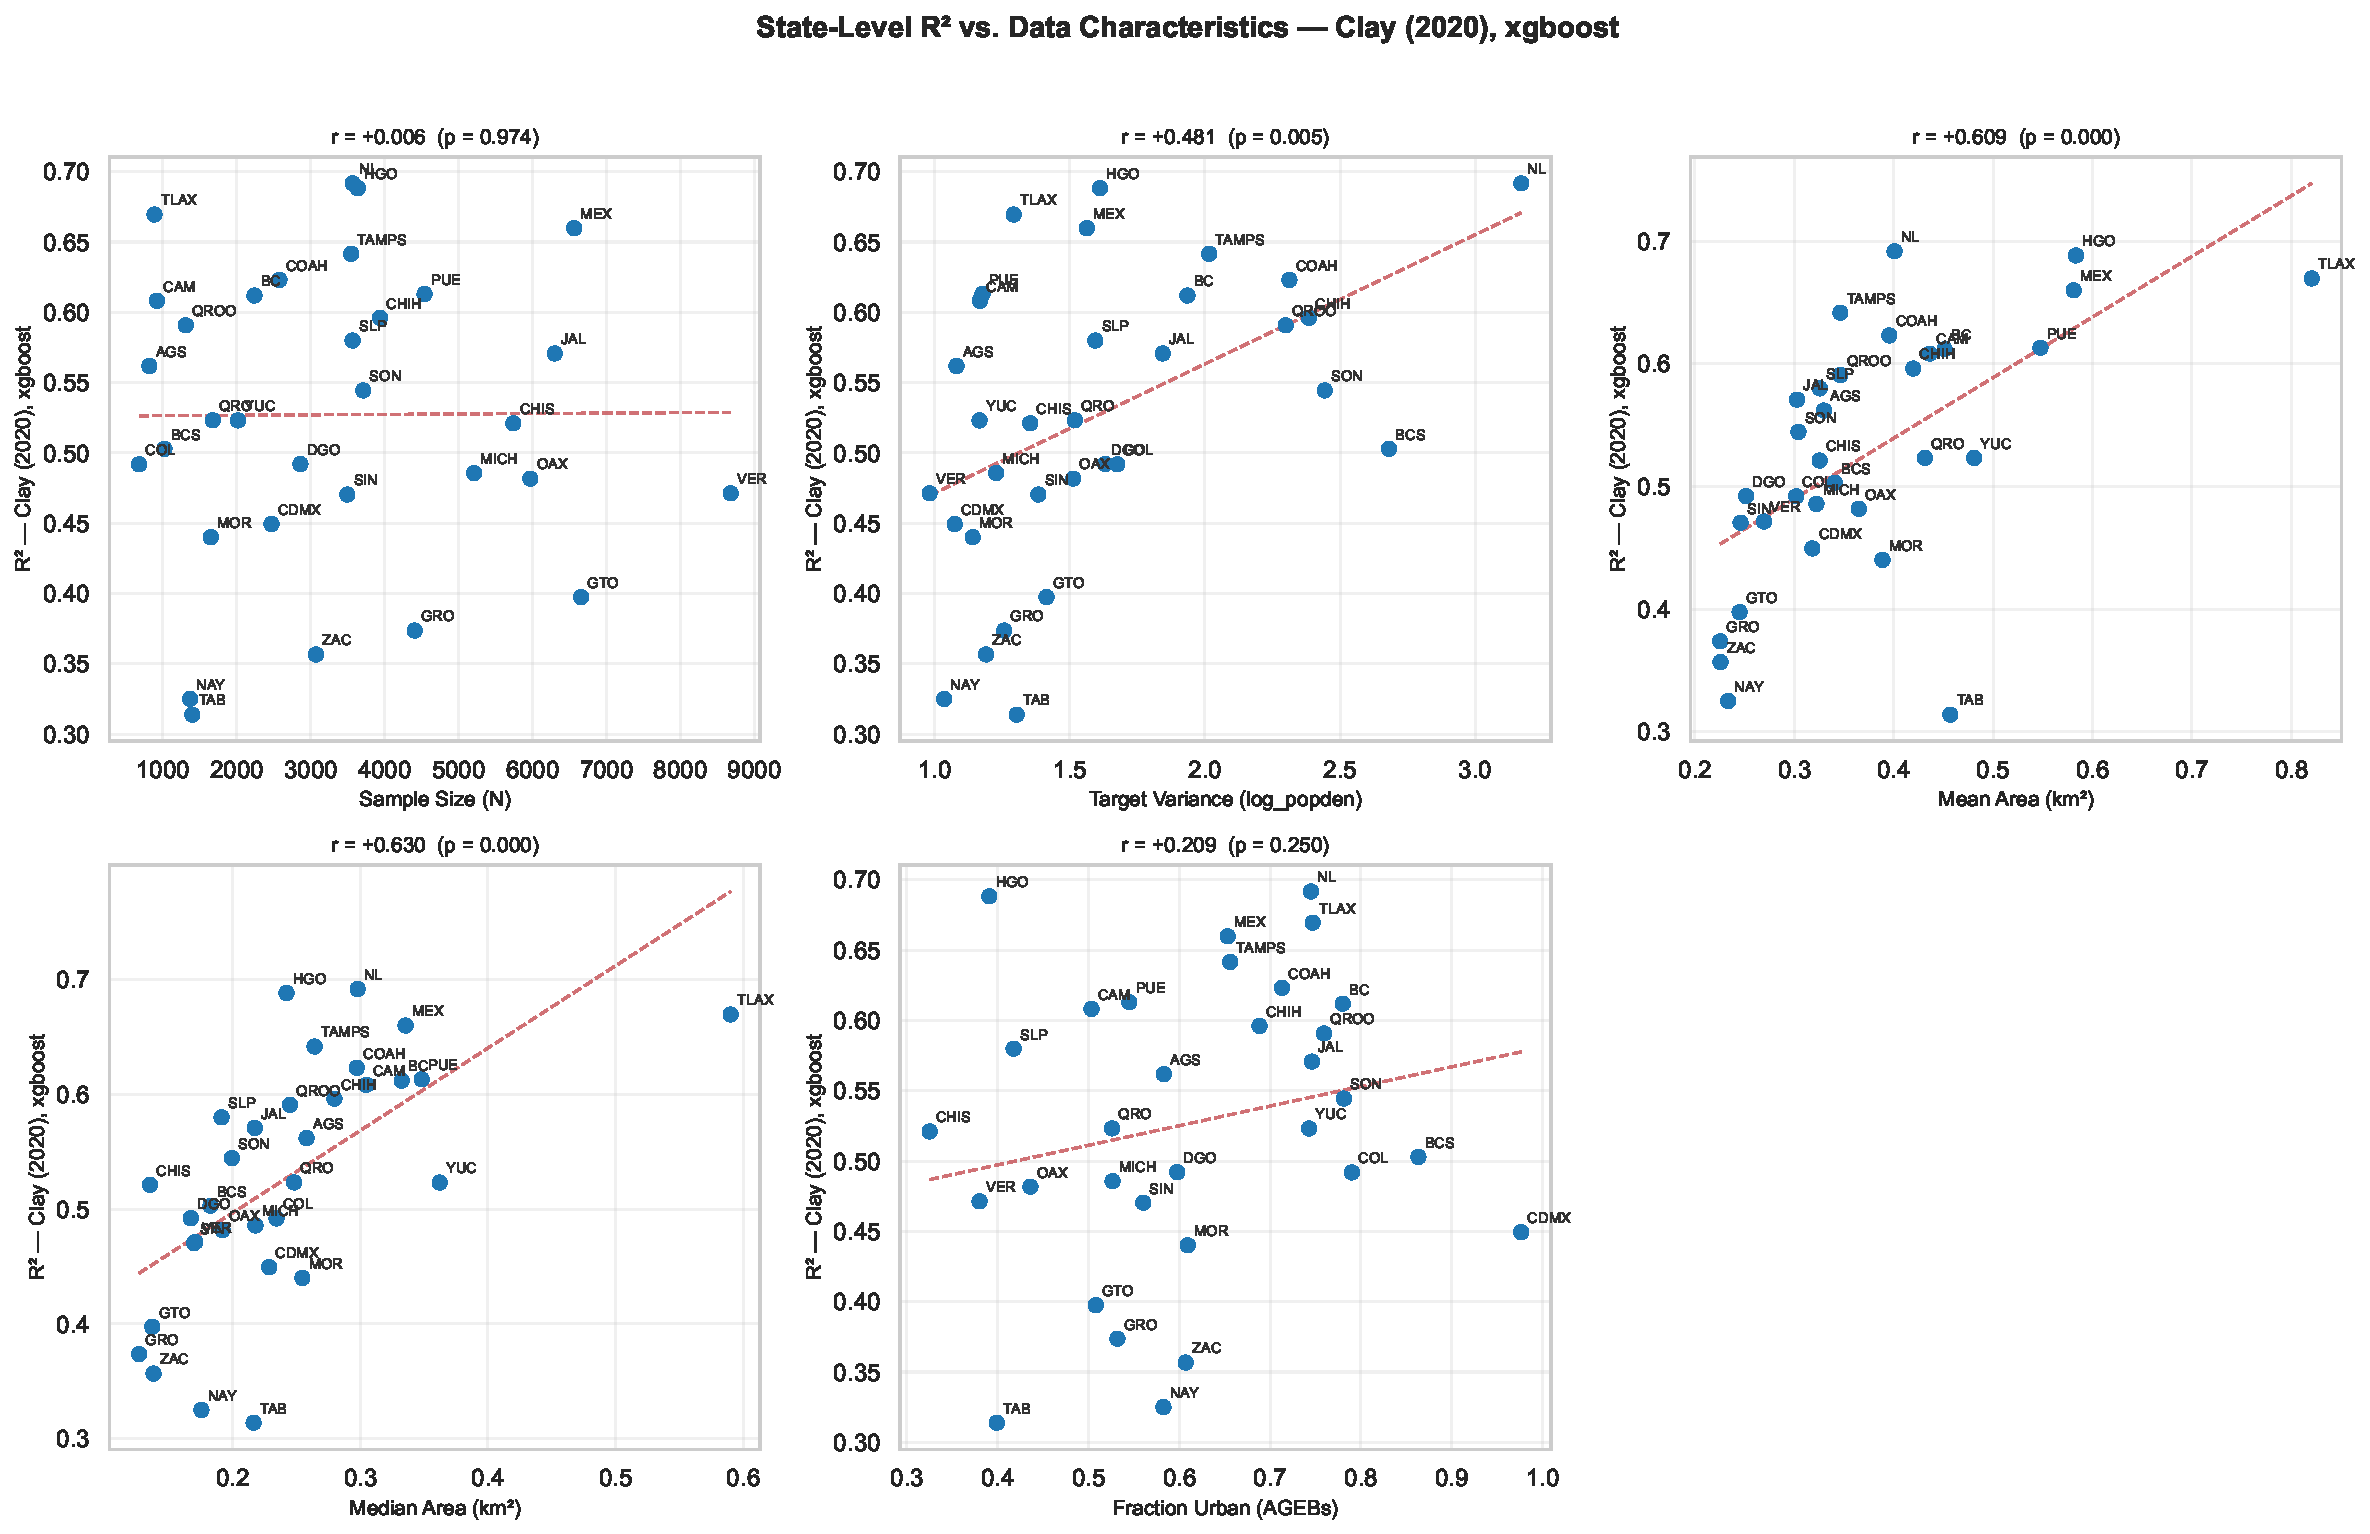
\includegraphics[width=\linewidth]{figs/state_r2_vs_characteristics_clay2020_xgboost.pdf}
    \caption{Clay, 2020 labels, XGBoost head.}
    \label{fig:state_r2_drivers_clay_2020_xgboost}
  \end{subfigure}
  \caption{State-level $R^2$ plotted against data characteristics (Clay 2020).}
\end{figure}


\end{document}
